\documentclass{article}
\usepackage{graphicx}
\usepackage{hyperref}
\usepackage[a4paper, total={7in, 10in}]{geometry} %6,10
\usepackage{float}
\usepackage[utf8]{inputenc}
\usepackage{listings}
\usepackage{xcolor}
\usepackage{amsmath}
\usepackage{amssymb}
\usepackage{multicol}
\usepackage{enumerate}
\usepackage{tikz}
\usepackage{mathtools}
\usepackage{array}
\usepackage{color, soul}
\usepackage{bbm}
\usetikzlibrary{positioning}
\DeclareMathOperator{\Tr}{Tr}
\newcommand*{\horzbar}{\rule[.5ex]{2.5ex}{0.5pt}}    % horizontal bar in matrices

\newcommand\undermat[2]{%
  \makebox[0pt][l]{$\smash{\underbrace{\phantom{%
    \begin{matrix}#2\end{matrix}}}_{\text{$#1$}}}$}#2}



\title{
    
\includegraphics[scale=0.6]{../images/LogoPoli2.jpg}\\[2cm]
    \huge{\textsc{Numerical Analysis for Machine Learning}}
    \author{\Large{\textsc{ Lorenzo Bozzoni \& Luigi Pagani }}\\
    }
  \date{Summer 2024}}




\begin{document}
%\begin{vplace}[0.7]
%  \maketitle
%\end{vplace}

\maketitle

\section*{Introduction}

These notes contain the lecture materials for the course in Numerical Analysis for Machine Learning held at Polytechnic University of Milan for the Academic Year 2023-2024. These notes are a reworked version of the notes originally produced by Lorenzo Bozzoni. Some content has been removed, some added, and some has been modified. I am also providing a link to the original notes and to the GitHub profile of the original author.\\ \\
\href{https://github.com/LorenzoBozzoni/NAML_notes}{GitHub Repository of the Original Notes}\\ \\
\href{https://github.com/LorenzoBozzoni}{GitHub of Lorenzo Bozzoni}
\newpage
\tableofcontents



\section{Row-reduced echelon form}
Given the matrix $A$, defined as follow:
\[
A = \begin{bmatrix}
    1 & 4 & 7\\
    2 & 5 & 8\\
    3 & 6 & 9
\end{bmatrix}
\]
we can obtain the \textbf{row-reduced echelon form} of $A$ by applying the following operations:
\[
A = CR = \begin{bmatrix}
1 & 4\\
2 & 5\\
3 & 6
\end{bmatrix}
\begin{bmatrix}
    1 & 0 & -1\\
    0 & 1 & 2
\end{bmatrix}
\]
where $C$ is the matrix containing the columns of $A$ that are linearly independent (i.e. $\mathcal{C}(A)$) and $R$ is the matrix of the coefficients of the linear combination of the columns of $A$ that gives the columns of $C$.\\

Let's now consider the following matrix:
\[
A_1 = \begin{bmatrix}
1 & 4\\
2 & 5\\
3 & 6
\end{bmatrix}  
\hspace{2cm}
A_1^\intercal = \begin{bmatrix}
1 & 2 & 3\\
4 & 5 & 6
\end{bmatrix}  
\]
What we can say about $A_1^\intercal$ column space? Is there any relationship with the column space of $A_1$?

In order to compute its column space, we can start noticing that: $\underline{a_3} = 2\underline{a_2} - \underline{a_1}$. So, in general, we can say that:
\[
dim(\mathcal{C}(A)) = dim(\mathcal{C}(A^\intercal)) = r \leq n \hspace{1cm} \text{where $n$ is the number of columns of $A$}
\]




\section{Factorizations}
\begin{enumerate}
    \item $A = LU$ or $PA = LU$
    \item $A = QR$ where $Q$ is orthogonal and $R$ is upper triangular
    This is an improved version of the Row-reduced echelon form because that worked only for square matrices, while this works for any matrix.
    \item Eigenvalues and eigenvectors decomposition: when $S = S^\intercal$ (symmetric matrix) we can factorize it as $S = Q\Lambda Q^\intercal$ where $\Lambda$ is a diagonal matrix and $Q$ is an orthogonal matrix (they are all squared matrices)
    \item Generalization of the above: $A = X\Lambda X^{-1}$ where $X$ is a non-orthogonal matrix
    \item $A = U\Sigma V^\intercal$ where $U$ and $V$ are orthogonal matrices and $\Sigma$ is a pseudo-diagonal matrix
\end{enumerate}
A matrix is said to be pseudo-diagonal if it has the following form:
\[
    \Sigma = 
    \begin{bmatrix}
        \sigma_1 & 0 & 0 & 0\\
        0 & \sigma_2 & 0 & 0\\
        0 & 0 & \ddots & 0\\
        0 & 0 & 0 & \sigma_n\\
        0 & 0 & 0 & 0\\
        \vdots & \vdots & \vdots & \vdots\\
        0 & 0 & 0 & 0
    \end{bmatrix}
    \hspace{2cm}
    m \text{ rows} \times n \text{ columns}
\]
So it has diagonal elements for the first $n$ rows then it has all zeros.

\subsection*{Orthogonal matrices}
A matrix $Q$ is orthogonal if $Q^\intercal Q = I$ (i.e. $Q^\intercal = Q^{-1}$). This means that the columns of $Q$ are orthonormal, i.e. they are orthogonal and have unit norm.\\

The determinant of a orthogonal matrix is $\pm 1$.

Properties:
\begin{itemize}
    \item $||Q\underline{x}|| = ||\underline{x}||$
    \item $||Q\underline{x}||^2 = (Q\underline{x})^\intercal Q\underline{x} = \underline{x}^\intercal \underbrace{Q^\intercal Q}_{I} \underline{x} = ||\underline{x}||^2$
\end{itemize}
The first property is particularly easy to interpret since it means that when we multiply an orthogonal matrix to a vector, the norm of the vector norm doesn't change. As a proof of this, we can consider the following examples:

\subsubsection*{Rotation}
A classical rotation matrix is:
\[
\begin{bmatrix}
    cos(\theta) & -sin(\theta)\\
    sin(\theta) & cos(\theta)
\end{bmatrix}    
\]
\subsubsection*{Reflection}
\begin{center}
    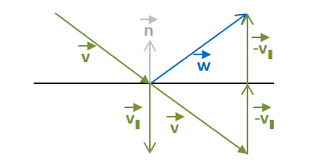
\includegraphics[scale=0.5]{../images/Reflection.png}
\end{center}
The horizontal line in the figure represent a plane $\pi$ while $\underline{n}$ is its normal vector of length 1. 
Given $\underline{v}$ to obtain $\underline{w}$ we can use the following formula:
\[
\underline{w} = \underline{v} - 2(\underline{v}^\intercal \underline{n})\underline{n} = \underbrace{(I - 2\underline{n}\underline{n}^\intercal)}_{\text{reflection matrix}}\underline{v}
\]
Moreover, $R^{-1} = R^\intercal$. This makes sense because if we apply the reflection matrix twice, we obtain the original vector $\underline{v}$, i.e. the reflection of the reflection is the starting vector.

If we didn't have the 2 in the formula, we would obtain the projection of $\underline{v}$ on the plane $\pi$ which is called orthogonal projection and the matrix $R$ would be singular. \\

Let's now dive a bit into the third point of the factorization list. We said that when $S = S^\intercal$ (symmetric matrix) we can factorize it as $S = Q\Lambda Q^\intercal$ where $\Lambda$ is a diagonal matrix and $Q$ is an orthogonal matrix.\\
\[
S = S^\intercal = \underbrace{(Q\Lambda))}_{\tilde{Q}}Q^\intercal = \tilde{Q}Q^\intercal   
\]
\[
\tilde{Q} = \underline{q_1}\underline{\lambda_1} + \dots + \underline{q_n}\underline{\lambda_n}    
\]
Where the $q$ vectors are columns and $\lambda$ vectors are rows. The notation here is a bit confusing but the not matrix $\tilde{Q}$ is not necessarily an orthogonal matrix, only if all eigenvalues of the matrix $\Lambda$ are unitary.
So we can reformulate:
\[
    S = (\underline{q_1}\underline{\lambda_1} + \dots + \underline{q_n}\underline{\lambda_n})Q^\intercal = \underline{q_1}\underline{\lambda_1}\underline{q_1}^\intercal + \dots + \underline{q_n}\underline{\lambda_n}\underline{q_n}^\intercal
\]
This is called \textbf{spectral decomposition} of matrix $S$ and $q_1, \dots, q_n$ are the eigenvectors of $S$ while $\lambda_1, \dots, \lambda_n$ are the eigenvalues of $S$.
\[
    S\underline{q_1} = \lambda_1\underline{q_1} = (\underline{q_1}\underline{\lambda_1}\underline{q_1}^\intercal + \dots + \underline{q_n}\underline{\lambda_n}\underline{q_n}^\intercal)\underline{q_1} = 
    \underline{\lambda_1}\underline{q_1}(\underline{q_1^\intercal}\underline{q_1})
    \]
All the other products are null since the vector $\underline{q_1}$ is orthogonal to all the other vectors $\underline{q_i}$ for $i \neq 1$ (recall that they are eigenvectors).

\section{Null spaces}
Let's consider the starting problem for a linear system of equations:
\[
A\underline{x} = \underline{b} \hspace{1cm} \text{with} \hspace{1cm} A\in \mathbb{R}^{m \times n}, \text{rank($A$)}=r    
\]

We are going to introduce 2 more spaces other than the column ones. To do so we consider:
\[
  A\underline{x} = \underline{0} \hspace{1cm} \rightarrow \hspace{1cm} N(A) \equiv \ker(A) = \{\underline{x} \in \mathbb{R}^n : A\underline{x} = \underline{0}\}  
\]
\[
    A^\intercal\underline{x} = \underline{0} \hspace{1cm} \rightarrow \hspace{1cm} N(A^\intercal) \equiv \ker(A^\intercal) = \{\underline{x} \in \mathbb{R}^n : A^\intercal\underline{x} = \underline{0}\}    
\]

So now, adding the so called \textbf{null spaces} we have that:
\begin{enumerate}
    \item $\mathcal{C}(A) \subset  \mathbb{R}^m$ and $dim(\mathcal{C}(A)) = r$
    \item $\mathcal{C}(A^\intercal) \subset \mathbb{R}^n$ and $dim(\mathcal{C}(A^\intercal)) = r$
    \item $N(A) \subset \mathbb{R}^n$ and $dim(N(A)) = ?$
    \item $N(A^\intercal) \subset \mathbb{R}^m$ and $dim(N(A^\intercal)) = ?$
\end{enumerate}
We still do not know the dimensions of those spaces. 
\subsection*{Null space cardinality}
In the first lecture, we defined 4 spaces: $N(A), N(A^\intercal), \mathcal{C}(A), \mathcal{C}(A^\intercal)$. For the last two we defined also their cardinality whilst for the first ones we weren't able to tell yet. In this lecture we are going to find those values and prove them. In order to do so, we start from few useful properties:
\begin{enumerate}
    \item $\underline{x} = \underline{0} \in N(A)$ for any matrix $A$
    \item if $\underline{x}, \underline{y} \in N(A) \implies A(\underline{x} + \underline{y}) = \underline{0}$
    \item if $\underline{x} \in N(A) \implies \alpha\underline{x}$ with $\alpha \in \mathbb{R} \implies A(\alpha\underline{x}) = \underline{0}$
\end{enumerate}  

Consider, once again, the matrix $A \in \mathbb{R}^{m\times n}$, rank($A$) = $r \leq n$. 
We have seen the decomposition $A = CR$, where $C$ contains the linearly independent columns of $A$ and $R$ contains the coefficients that allow to recover the columns of $A$ starting from its independent columns. 
So, the matrix $A$ can be rewritten as:
\[
  A = \begin{bmatrix}
    A_1 & A_2
  \end{bmatrix} 
  \hspace{1cm}
  A_1 \in \mathbb{R}^{m\times r} \hspace{1cm} A_2 \in \mathbb{R}^{m\times (n-r)} 
\]
Where $A_1$ contains the independent columns of $A$ and $A_2$ the dependent ones.
Example:
\[
A = 
\begin{bmatrix}
    1 & 4 & 7\\
    2 & 5 & 8\\
    3 & 6 & 9
\end{bmatrix}
= 
\underbrace{
\begin{bmatrix}
1 & 4\\
2 & 5\\
3 & 6
\end{bmatrix}}_{A_1}
\begin{bmatrix}
    1 & 0 & -1\\
    0 & 1 & \undermat{B}{2}
\end{bmatrix}
\]
Since we have the last column of $A$, that is linearly dependent so it belongs to $A_2$, we can reformulate it in this way:
\[
    A = \begin{bmatrix}
        A_1 & A_2
      \end{bmatrix} 
    = \begin{bmatrix}
        A_1 & A_1B
    \end{bmatrix}
\]
We build a new matrix $K$ defined as follows:
\[
    K = \begin{bmatrix}
        -B\\
        I_{n-r}
    \end{bmatrix}
    \hspace{1cm}
    K \in \mathbb{R}^{n\times(n-r)}    
    \hspace{1cm}
    B \in \mathbb{R}^{r\times(n-r)}    
\]

\[
AK = \begin{bmatrix}
    A_1 & A_1B
\end{bmatrix} 
\begin{bmatrix}
    -B\\
    I_{n-r}
\end{bmatrix}
= A_1(-B) + A_1B = 0   
\]
Where the last 0 is actually a matrix of zeros of dimension $m\times(n-r)$
because A has size $m\times n$ and $K$ has size $n\times(n-r)$.
We have that:
\[
    AK = 0 \implies A\underline{k_i} = 0 \hspace{1cm} \forall i \in \{1, \dots, n-r\}    
\]
Where $k_i$ is the i-th column of $K$. This means that: $\underline{k_i} \in N(A) \hspace{0.2cm} \forall i$.

Now, we want to demonstrate that: $K\underline{u} = 0 \implies \underline{u} = \underline{0}$. 
To do so, we start from expanding $K$ from its definition:
\[
    K = \begin{bmatrix}
        -B\\
        I
    \end{bmatrix}
    \underline{u} = 0
    \implies
    \begin{bmatrix}
        -B\underline{u}\\
        \underline{u}
    \end{bmatrix}
    = 
    \begin{bmatrix}
        \underline{0}\\
        \underline{0}
    \end{bmatrix}
\]
Where the two zero vectors have dimension $r$ and $n-r$ respectively! Considering the second row of the matrix we get: $\underline{u} = \underline{0}$ so all columns of $K$ are linearly independent.\\

If we consider the problem ($\star$) $A\underline{x} = \underline{0}$, we want to prove that each \underline{x} that satisfy ($\star$) must be a linear combination of the columns of $K$.\\
\[
    A_1\underline{x} = \underline{0} \in \mathbb{R}^m \implies \underline{x} = \underline{0} \in \mathbb{R}^r    
\]
Because $A_1$ has linearly independent columns, i.e. has full rank.
\[
    A\underline{u} = \underline{0} \in \mathbb{R}^m \implies \begin{bmatrix}
        A_1 & A_1B
    \end{bmatrix} 
    \begin{bmatrix}
        \underline{u_1}\\
        \underline{u_2}
    \end{bmatrix}  
    = 
    \begin{bmatrix}
        A_1\underline{u_1} + A_1B\underline{u_2}\\
    \end{bmatrix}
    = 
    A_1\left[\underline{u_1} + B\underline{u_2}\right]
    = \underline{0}
\]
We can notice that the last formulation obtained in the equation has the same form as the one from where we started the proof, so we can say that:
\[
    \underline{u_1} + B\underline{u_2} = \underline{0} \implies \underline{u_1} = -B\underline{u_2}    
\]
\[
   \underline{u} = \begin{bmatrix}
    -B\underline{u_2}\\
    \underline{u_2}
\end{bmatrix}
    =
\underbrace{\begin{bmatrix}
    -B\\
    I
\end{bmatrix}}_{K}
    \underline{u_2}
    = K\underline{u_2}
    \implies 
    dim(N(A)) = n - r
\]


\begin{center}
    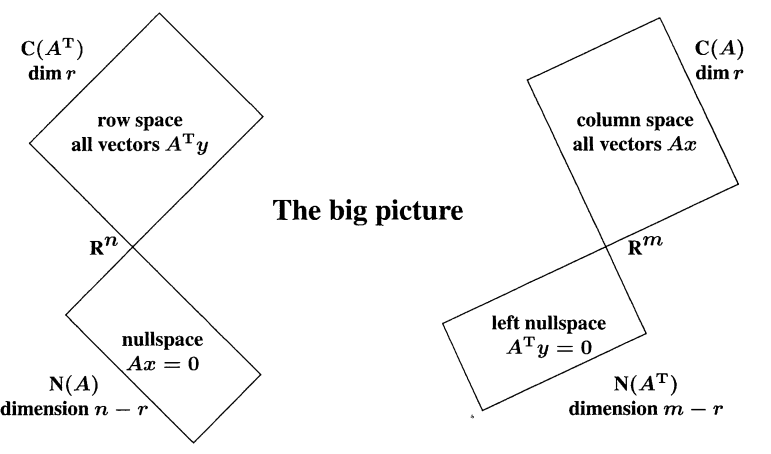
\includegraphics[scale = 0.4]{../images/SpacesDimensions.png}
\end{center}


\\





\section{Eigenvalues and eigenvectors}
Start considering a generic square matrix $n \times n$. We are going later to discuss even the simmetry and positive definite properties.
Here below are the vectorial and the matrix form of the eigenvalue problem:
\[
    A\underline{x_i} = \lambda_i\underline{x_i} \hspace{0.5cm} i = 1, \dots, n \hspace{1cm} X^{-1}AX = \Lambda
\]
Where in the right-hand side there is a diagonal matrix $\Lambda$ with the eigenvalues of $A$ on the diagonal while the matrix $X$ with the eigenvectors of $A$ as columns.\\

\subsection*{Eigenvectors of matrix power}
What can we say about the eigenvectors and eigenvalues of $A^2$?
\[
    A^2\underline{x_i} = A(A\underline{x_i}) = A(\lambda_i\underline{x_i}) = \lambda_i(A\underline{x_i}) = \lambda_i^2\underline{x_i}    
\]
So the eigenvalues of $A^2$ are the eigenvalues of $A$ squared. This is valid for any power of $A$ since this method can be applied recursively and it is very useful when there are problems in which a matrix is iteratively multiplied many times. \\

\textbf{Important}:\\
Given $A\in \mathbb{R}^{n\times n}$ full rank, then any vector $\underline{v} \in \mathbb{R}^n$ can be written as a linear combination of the eigenvectors ($x_i$) of $A$.\\
\subsection*{Power Method}
In mathematics, the Power Method (also known as Power Iteration) is an eigenvalue algorithm designed to find the largest eigenvalue in absolute value, \(\lambda\), of a diagonalizable matrix \(A\). This algorithm also identifies a corresponding nonzero eigenvector \(v\), such that \(Av = \lambda v\). This method is sometimes referred to as the Von Mises iteration.

Additionally, the \textbf{Inverse Power Method} targets the smallest eigenvalue by applying the Power Method to \(A^{-1}\), and the \textbf{Power Method with a Shift} applies to \((A - \alpha I)^{-1}\) for \(\alpha \in \mathbb{R}\), aiming to find the eigenvalue closest to \(\alpha\).

The algorithm can also be used iteratively in a "deflation method" to find other eigenvalues by restructuring the matrix as follows:
\[
\begin{bmatrix}
    \lambda_1 & \underline{b_1^\top} \\
    0 & A_1
\end{bmatrix}
\]
Here, \(\lambda_1\) is an eigenvalue, \(\underline{b_1^\top}\) is a row vector, and \(A_1\) is the submatrix for subsequent iterations. This technique assumes distinct eigenvalues and eigenvectors for each iteration. The method's efficacy depends on the matrix's ability to be reduced in this manner and may vary based on the distinctiveness and properties of the eigenvectors.


\subsection*{Similar matrices}
Given two matrices $A, B \in \mathbb{R}^{n \times n}$, they are said to be similar if there exists an invertible matrix $M$ such that $B = M^{-1}AM$. Let $\lambda$ and $\underline{y}$ be an eigenvalue and corresponding eigenvector of $B$, respectively. Then:
\[
    \underbrace{M^{-1}AM}_{B}\underline{y} = \lambda \underline{y} \implies AM\underline{y} = \lambda M\underline{y}
\]
Let $\underline{w} = M\underline{y}$. Then:
\[
    A\underline{w} = \lambda \underline{w}
\]
This equation shows that $\underline{w}$ is an eigenvector of $A$ with the same eigenvalue $\lambda$. Therefore, \textbf{similar matrices share the same eigenvalues, and their eigenvectors are related by the similarity transformation matrix $M$}.

\subsection*{QR factorization}
 Let's consider a matrix $A \in \mathbb{R}^{m\times n}$ where $m \geq n$ and $rank(A) = n$ (it has all independent columns). We can factorize $A$ in this way:
\[
    A = QR \hspace{1cm} Q \in \mathbb{R}^{m\times n} \hspace{1cm} R \in \mathbb{R}^{n\times n}
\]
Where is $Q$ is an orthogonal matrix and $R$ is an upper triangular matrix. Since we are dealing with eigenvalues and eigenvectors, we are now going to consider the matrix $A$ squared with the dimension $n\times n$.

\subsubsection*{QR iteration}
The QR iteration is a method for finding the eigenvalues of a matrix. Let's start with a matrix $A$ and perform the initial QR decomposition:
\[
    A = A^{(0)} = Q^{(0)}R^{(0)}
\]
where $Q^{(0)}$ is an orthogonal matrix and $R^{(0)}$ is an upper triangular matrix. We then update $A$ by multiplying $Q^{(0)T}$ and $A^{(0)}$, and then multiplying the result by $Q^{(0)}$:
\[
    A^{(1)} = {Q^{(0)}}^{\intercal} A^{(0)} Q^{(0)} = Q^{(1)} R^{(1)}
\]
Iterating this procedure, we get:
\[
    A^{(2)}, \dots, A^{(S)} \text{, where } A^{(S)} \text{ is approximately upper triangular}
\]
After $S$ iterations, the matrix $A^{(S)}$ becomes approximately upper triangular. The matrices $A, A^{(0)}, A^{(1)}, \dots, A^{(S)}$ are similar, so they share the same eigenvalues.

To compute the orthogonal matrix $Q$ at each iteration, we use the \textbf{Gram-Schmidt} procedure. This procedure works for both square and non-square matrices.

Let's start with a generic matrix $A$:
\[
    A = \begin{bmatrix}
        \vline & \vline & \vline\\
        \underline{a_1} & \ldots & \underline{a_n}\\
        \vline & \vline & \vline
    \end{bmatrix}
\]
The Gram-Schmidt algorithm is iterative and is applied to the columns of $A$ as follows:

First, normalize the first column of $A$ to obtain $\underline{q_1}$:
\[
  \underline{q_1} = \frac{\underline{a_1}}{||\underline{a_1}||}
\]
The vector $\underline{q_1}$ will have a norm of 1.

Next, subtract the projection of $\underline{a_2}$ onto $\underline{q_1}$ from $\underline{a_2}$, and normalize the result to obtain $\underline{q_2}$:
\[
    \underline{q_2} = \underline{a_2} - \underline{q_1}(\underline{q_1}^\intercal \underline{a_2}) \implies \underline{q_2} = \dfrac{\underline{q_2}}{||\underline{q_2}||}
\]
The new vector $\underline{q_2}$ will be orthogonal to $\underline{q_1}$ and have a norm of 1.

For the third column, subtract the projections of $\underline{a_3}$ onto $\underline{q_1}$ and $\underline{q_2}$, and normalize the result to obtain $\underline{q_3}$:
\[
    \underline{q_3} = \underline{a_3} - \underline{q_1}(\underline{q_1}^\intercal \underline{a_3}) - \underline{q_2}(\underline{q_2}^\intercal \underline{a_3}) \implies \underline{q_3} = \dfrac{\underline{q_3}}{||\underline{q_3}||}
\]
Continue this process for the remaining columns of $A$. The resulting matrix $Q$ will be orthogonal and orthonormal, meaning that its columns will be orthogonal to each other and have unit norm. This orthogonality is necessary to obtain the orthogonal matrix $Q$ for the QR decomposition.\\
Let's now continue with the factorization journey. In the introduction to types of factorizations, we mentioned that given a square matrix $A \in \mathbb{R}^{n \times n}$, we have:
\[
    A = X \Lambda X^{-1}
\]
where $X$ has the eigenvectors of $A$ as its columns, and $\Lambda$ is a diagonal matrix with the eigenvalues of $A$ on its diagonal. Now, let's consider the case where the matrix $S$ is symmetric:
\[
    S \in \mathbb{R}^{n\times n}, \quad S = S^\intercal
\]
For a symmetric matrix $S$, we can factorize it as follows:
\[
    S = Q \Lambda Q^\intercal
\]
where $Q$ is an orthogonal matrix (i.e., $Q^\intercal Q = Q Q^\intercal = I$) and $\Lambda$ is a diagonal matrix. The orthogonality of $Q$ is a direct consequence of $S$ being symmetric. We can prove this property by considering two cases:

\begin{enumerate}
    \item Let $\underline{x}$ and $\underline{y}$ be two eigenvectors of $S$ such that $S\underline{x} = \lambda\underline{x}$ and $S\underline{y} = 0\underline{y}$. In other words, $\underline{y}$ corresponds to a zero eigenvalue, and $\underline{x}$ corresponds to a non-zero eigenvalue. We have:
    \[
        \begin{rcases}
            \underline{y} \in N(S) \\
            \underline{x} \in \mathcal{C}(S) = \mathcal{C}(S^{\intercal})    
        \end{rcases}
        \implies \underline{x} \perp \underline{y}
    \]

    
    \item Now, consider two eigenvectors $\underline{x}$ and $\underline{y}$ corresponding to different non-zero eigenvalues $\lambda$ and $\alpha$, respectively. We have $S\underline{x} = \lambda\underline{x}$ and $S\underline{y} = \alpha\underline{y}$. Consider the matrix $(S - \alpha I)$:
    \[
        (S - \alpha I)\underline{y} = 0\underline{y} \implies \underline{y} \in N(S - \alpha I)
    \]
    \[
        (S - \alpha I)\underline{x} = (\lambda - \alpha)\underline{x} \implies \underline{x} \in \mathcal{C}(S - \alpha I) = \mathcal{C}((S - \alpha I)^{\intercal})
    \]
    Once again, we conclude that $\underline{x} \perp \underline{y}$.
\end{enumerate}

Another important property of symmetric matrices is that their eigenvalues are real, i.e., $\lambda_i \in \mathbb{R}$. To prove this, consider the eigenvalue equation:
\[
    S\underline{x} = \lambda\underline{x} \implies \overline{\underline{x}}^\intercal S\underline{x} = \lambda\overline{\underline{x}}^\intercal\underline{x}
\]
Here, $\overline{\underline{x}}$ represents the conjugate of the vector $\underline{x}$. If $\underline{x}$ has complex components, those elements are conjugated; otherwise, they remain unchanged. The product of a complex number and its conjugate always yields a real number:
\[
    (a + ib)(a - ib) = (a^2 + b^2) \in \mathbb{R}    
\]
From the eigenvalue equation, we obtain:
\[
    \lambda = \frac{\overline{\underline{x}}^\intercal S\underline{x}}{\overline{\underline{x}}^\intercal\underline{x}} \in \mathbb{R}
\]
We can conclude that the term in the numerator is also real. This is because, for a Hermitian matrix \( S \), which is equal to its own conjugate transpose, the following holds:
\[ (x^* S x)^* = x^* S^* x = x^* S x \]
This equality implies that \( x^* S x \) is equal to its own complex conjugate. For a scalar quantity, being equal to its own complex conjugate means that it is real. Therefore, \( x^* S x \) must be real. Where here the term $x^*$ is the complex conjugate of x, equivalent to $\underline{x}^\intercal$.
This proves that the eigenvalues of a symmetric matrix are real.\\ 
In summary, symmetric matrices have two important properties:
\begin{itemize}
    \item Their eigenvectors are orthogonal, leading to an orthogonal matrix \( Q \) in the eigendecomposition.
    \item Their eigenvalues are real.
\end{itemize}


\subsection*{Positive-definite symmetric matrices (SPD)}
Properties of symmetric matrices:
\begin{enumerate}[i]
    \item $\lambda_i > 0 \hspace{0.5cm} \forall i = 1, \dots, n$
    \item $\underline{v}^\intercal S \underline{v} \geq 0 \hspace{0.5cm} \forall \underline{v} \in \mathbb{R}^n$, with equality if and only if $\underline{v} = 0$
    \item Leading determinants are positive. \\
    \begin{multicols}{2}
        \begin{center}
            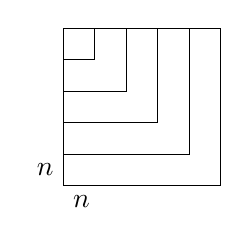
\begin{tikzpicture}
                \draw (0,0) -- (2,0) -- (2,2) -- (0,2) -- (0,0);
                \draw (0,0.4) -- (1.6,0.4) -- (1.6,2) -- (0,2) -- (0,0);
                \draw (0,0.8) -- (1.2,0.8) -- (1.2,2) -- (0,2) -- (0,0); 
                \draw (0,1.2) -- (0.8,1.2) -- (0.8,2) -- (0,2) -- (0,0) node[above left]{$n$};
                \draw (0,1.6) -- (0.4,1.6) -- (0.4,2) -- (0,2) -- (0,0) node[below right]{$n$};
            \end{tikzpicture}
        \end{center}

        This means that the determinant of the matrix obtained by taking the first $k$ rows and columns of $S$ is positive, $\forall k = 1, \dots, n$.
    \end{multicols}

    \item Cholesky decomposition: $S = B^\intercal B$, with $B$ upper triangular
    \item All pivot elements are positive in the Gaussian elimination process
\end{enumerate}

\paragraph{Proof that a Symmetric matrix is Positive Definite}
Since \(\underline{x}\) is an eigenvector and \(\underline{v}\) is a generic vector, we express \(\underline{v}\) as a linear combination of the eigenvectors of \(S\):
\[
\underline{v} = c_1 \underline{x}_1 + c_2 \underline{x}_2 + \dots + c_n \underline{x}_n
\]
Then,
\[
(c_1 \underline{x}_1 + c_2 \underline{x}_2 + \dots + c_n \underline{x}_n)^\intercal S (c_1 \underline{x}_1 + c_2 \underline{x}_2 + \dots + c_n \underline{x}_n)
\]
Expanding this, we get two types of components:
\[
\begin{cases}
c_1^2 \underline{x}_1^\intercal S \underline{x}_1 = c_1^2 \lambda_1 \|\underline{x}_1\|^2\\
c_1 c_2 \underline{x}_1^\intercal S \underline{x}_2 = c_1 c_2 \lambda_2 \underline{x}_1^\intercal \underline{x}_2 = 0 \text{ (orthogonal)}
\end{cases}
\]

This shows that \(S\) is positive semi-definite

This property can also be proved from \textit{iv}):
\[
    S = B^\intercal B \implies \underline{v}^\intercal(B^\intercal B)\underline{v} = (\underline{v}^\intercal B^\intercal)(B \underline{v}) = (B\underline{v})^\intercal (B\underline{v}) = ||B\underline{v}||^2 \geq 0   
\]


\section{Singular Value Decomposition (SVD)}
We are going to use it for:
\begin{itemize}
    \item Least-squares approximation by introducing the pseudo-inverse of a matrix (Moore-Penrose inverse)
    \item Low-rank approximation with the Eckart-Young theorem
\end{itemize}
We start from:
\[
A \in \mathbb{R}^{m \times n} \hspace{1cm} 
\begin{cases}
m = \text{\# of samples}\\
n = \text{\# of features}
\end{cases}    
\]
We can write:
\[
    A = U\Sigma V^\intercal    
\]
With:
\begin{itemize}
    \item $U$ with dimensions $m \times m$ and orthogonal
    \item $\Sigma$ with dimensions $m \times n$ \textit{almost} diagonal
    \item $V^\intercal$ with dimensions $n \times n$ and orthogonal
\end{itemize}
If $m > n$, we can represent the matrices like this:
\[
\underbrace{
  \begin{bmatrix}
    & & & & & \\
    & & & & & \\
    & & & & & \\
    & & & & & \\
    & & & & & \\
  \end{bmatrix}}_{m \times m}
\underbrace{
  \begin{bmatrix}
    & & & \\
    & & & \\
    & & & \\
    & & & \\
    & & & \\
  \end{bmatrix}}_{m \times n}
\underbrace{
  \begin{bmatrix}
    & & & \\
    & & & \\
    & & & \\
  \end{bmatrix}}_{n \times n}
\]
What is the idea of SVD? Try to change features so variances are maximized and covariances are minimized. We don't want columns to be correlated.\\

In general: rank($A$) = $r < n$.
\[
    AV = U\Sigma \impliedby V^\intercal V = I \impliedby V \text{ is orthogonal}    
\]
The component wise notation is:
\[
    A\underline{v_i} = \sigma_i\underline{u_i}    
\]
Given that the rank of $A$ is $r$:

\[
\begin{bmatrix}
    & & & & & & &\\
    & & & & & & &\\
    & & & & & & &\\
    & & & & & & &\\
    & & & & & & &\\
    & & & & & & &\\
\end{bmatrix}
\begin{bmatrix}
    \sigma_1 & & & &\\
    & \sigma_2 & & &\\
    & & \ddots & &\\
    & & & \sigma_r &\\
    & & & & 0\\
    \hline
    0 & 0 & 0 & 0 & 0\\
    0 & 0 & 0 & 0 & 0\\
\end{bmatrix}
\begin{bmatrix}
    & & & & \\
    & & & & \\
    & & & & \\
    & & & & \\
\end{bmatrix}
\hspace{1cm}
\begin{cases}
\sigma_1, \dots, \sigma_r > 0\\
\sigma_{r+1}, \dots, \sigma_n = 0
\end{cases}  
\]

So the first $r$ vectors span the column space of $A$ while for the last $n-r$ means that $\underline{v_i} \in N(A)$ for $i = r+1, \dots, n$.
If we have $A^\intercal$, the decomposition is $A^\intercal = (U\Sigma V^\intercal)^\intercal = V\Sigma^\intercal U^\intercal$. 

\subsection*{Economy SVD}
What we've seen so far is the full SVD, but it can be optimized. Here is following the compact (reduced) representation, where once again we consider $m > n$:
\[
\underbrace{
  \begin{bmatrix}
    & & & \\
    & & & \\
    & & & \\
    & & & \\
    & & & \\
  \end{bmatrix}}_{m \times n}
\underbrace{
  \begin{bmatrix}
    & & & \\
    & & & \\
    & & & \\
  \end{bmatrix}}_{n \times n}
\underbrace{
  \begin{bmatrix}
    & & & \\
    & & & \\
    & & & \\
  \end{bmatrix}}_{n \times n}
\]
This is caused by the fact that the last $m-n$ rows in the central matrix are all 0 so multiply them for the last $m-n$ columns of the left matrix is useless. This can be furthermore optimized by having matrix dimensions: $(m\times r)(r\times r)(r\times n)$ because not all $\sigma$ might be different than 0 (i.e. the rank of $A$ is $r$), so, in that case is useless even to multiply the last $m-r$ rows of the central matrix. \\

\textbf{The SVD works for any matrix $A$.}\\

\noindent Let's suppose $A$ is full rank $n\times n$:
\[
    A = U\Sigma V^\intercal = \sum_{i = 1}^{n} \sigma_i \underbrace{\underline{u_i}\underline{v_i}^\intercal}_{\text{rank }=1}    
\]
If $A$ is not full rank but instead has rank($A$)=$r$, the same sum is no more computed until $n$, but instead $r$.
\[
    A = \sum_{i = 1}^{r} \sigma_i \underline{u_i}\underline{v_i}^\intercal   
\]
What happens now if we pick a certain value $\tilde{r} < r$?
\[
    A = U\Sigma V^\intercal \cong \sum_{i = 1}^{\tilde{r}} \sigma_i \underline{u_i}\underline{v_i}^\intercal   
\]
We obtain a \textbf{rank $\tilde{r}$ approximation of the matrix A}. The rank of the matrix is known because is the sum of $\tilde{r}$ matrices of rank 1. Moreover, that one, is the best approximation of rank $\tilde{r}$ possible, i.e.:
\[
    ||A - \tilde{A}|| \leq ||A - B|| \hspace{1cm} \forall B  \text{ of rank} = \tilde{r}    
\]

\subsection*{Proof that $ U\Sigma^2 U^T$ }
Once again, we start from matrix $A \in \mathbb{R}^{m \times n}$ and rank$=r$. We consider the new matrix $A^\intercal A$ which is:
\begin{itemize}
    \item symmetric: $(A^\intercal A)^\intercal = A^\intercal A$
    \item positive definite: $\underline{x}^\intercal(A^\intercal A)\underline{x} = (\underline{x}^\intercal A^\intercal)(A \underline{x}) = (A\underline{x})^\intercal (A\underline{x}) = ||A\underline{x}||^2 \geq 0  $
\end{itemize} 
We can use the following decomposition:
\[
    A^\intercal A = V\Lambda V^\intercal = \sum_{i=1}^n \lambda_i \underline{v_i} \underline{v_i^\intercal}    
\]
Recall that $V$ contains the eigenvectors while $\Lambda$ contains the eigenvalues. We rename $\lambda_i = \sigma_i^2$. The rank of $A^\intercal A$ is $r$.\\

We want to prove that if  $\underline{x} \in N(A)$ then $\underline{x} \in N(A^\intercal A)$, to do so we proceed in both directions:
\begin{enumerate}
    \item If we have $A\underline{x} = 0 \implies \underline{x} \in N(A)$. Is it possible to multiply both terms:
    \[
        A^\intercal(A\underline{x}) = A^\intercal \underline{0} = \underline{0} \hspace{1cm} \text{so} \hspace{1cm} \underline{x} \in N(A) \implies \underline{x} \in N(A^\intercal A)
    \]
    \item We start from $(A^\intercal A)\underline{x} = 0 \implies \underline{x} \in N(A^\intercal A)$. Again, we multiply:
    \[
        \underline{x}^\intercal A^\intercal A\underline{x} = ||A\underline{x}||^2 = 0 \hspace{1cm} \text{so} \hspace{1cm} \underline{x} \in N(A^\intercal A) \implies \underline{x} \in N(A)
    \]
\end{enumerate}
Let's consider the couple of (eigenvalues, eigenvectors) = ($\sigma_i^2, \underline{v_i}$):
\[
    A^\intercal A\underline{v_i} = \sigma_i^2 \underline{v_i} \hspace{0.3cm}\overset{\text{component-wise}}{\longrightarrow} \hspace{0.3cm} A^\intercal A\underline{v_i} = \sigma_i^2 \underline{v_i} \hspace{1cm} (\dagger)
\]
We introduce the quantity $\underline{u_i} = \dfrac{A\underline{v_i}}{\sigma_i}$ which has some characteristics:
\begin{enumerate}[i]
    \item $\underline{u_i}$ are unitary vectors:
    \[
        \underline{u_i}^\intercal \underline{u_i} = \left(\dfrac{A\underline{v_i}}{\sigma_i}\right)^\intercal \left(\dfrac{A\underline{v_i}}{\sigma_i}\right) = \dfrac{\underline{v_i^\intercal}A^\intercal A\underline{v_i}}{\sigma^2} \overset{\dagger}{=} \dfrac{\sigma_i^2 \underline{v_i^\intercal}\underline{v_i}}{\sigma_i^2} = 1
    \]
    The last passage of the equation is true because $\underline{v_i}$ vectors are orthonormal.
    \item $\underline{u_i} \perp \underline{u_j}$:
    \[
        \underline{u_i}^\intercal \underline{u_j} = \left(\dfrac{A\underline{v_i}}{\sigma_i}\right)^\intercal \left(\dfrac{A\underline{v_j}}{\sigma_j}\right) = \dfrac{\underline{v_i^\intercal}A^\intercal A\underline{v_j}}{\sigma_i \sigma_j} \overset{\dagger}{=} \dfrac{\sigma_j^2 \underline{v_i^\intercal}\underline{v_j}}{\sigma_i \sigma_j} = 0
    \] 
    \item $\underline{u_i}$ are eigenvectors of $AA^\intercal$ with eigenvalues $\sigma_i^2$:
    \[
        (AA^\intercal \underline{u_i}) = AA^\intercal\left(\dfrac{A\underline{v_i}}{\sigma_i}\right) = A\dfrac{A^\intercal A\underline{v_i}}{\sigma_i} \overset{\dagger}{=} A\dfrac{\sigma_i^2 \underline{v_i}}{\sigma_i} = \sigma_i^2\left(\dfrac{A\underline{v_i}}{\sigma_i}\right) = \sigma_i^2\underline{u_i}   
    \]
\end{enumerate}
We have demonstrated that $A\underline{v_i} = \sigma_i \underline{u_i}$ and $A^T\underline{u_i} = \sigma_i \underline{v_i}$ a $\underline{u_i}$ are orthonormal as well. 

We have seen that $\underline{u_i} = \frac{A\underline{v_i}}{\sigma_i}$ but, what happen if $\sigma_i = 0$?\\
Until now we have assumed that could not happen.
A concise recap of all versions of SVD:
\begin{enumerate}
    \item \textbf{full SVD}: $\underset{(m \times n)}{A} = \underset{(m \times m)}{U}\underset{(m \times n)}{\Sigma}\underset{(n \times n)}{V^\intercal}$
    \item \textbf{economy SVD}: $\underset{(m \times n)}{A} = \underset {(m \times n)}{U}\underset{(n \times n)}{\Sigma}\underset{(n \times n)}{V^\intercal}$
    \item \textbf{reduced SVD}: $\underset{(m \times n)}{A} = \underset{(m \times r)}{U}\underset{(r \times r)}{\Sigma}\underset{(r \times n)}{V^\intercal}$
    \item \textbf{truncated SVD approximation}: $\sum\limits_{i=1}^{\tilde{r}} \sigma_i\underline{u_i}\underline{v_i^\intercal}$
\end{enumerate}
For the first two cases the rank of $A$ is $n$, for the third is $r$ while in the first the approximation rank is decided.

\subsection*{Geometrical interpretation of SVD}
Matrices \( U \) and \( V^\intercal \) are orthonormal, so as mentioned in the section above, they represent rotations (or reflections), while \( \Sigma \), being a diagonal matrix, corresponds to a scaling transformation. 
\begin{center}
    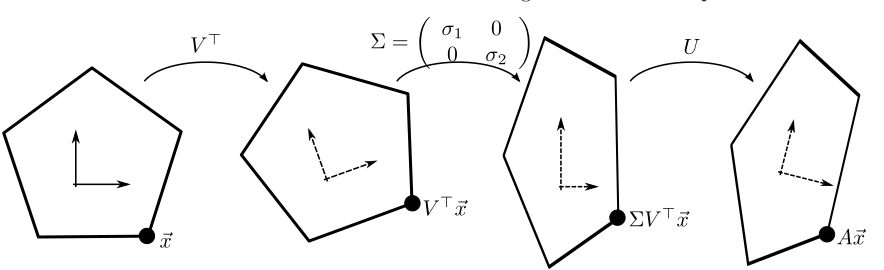
\includegraphics[scale=0.4]{../images/SVD_Geometric_Interpretation.png}
\end{center}
\textbf{Since for SVD no assumptions are made on the starting matrix, this means that \underline{any} matrix can be obtained from two rotations (or reflections) and one scaling.}


For any square matrix we can apply the \textbf{polar decomposition}:
\[
A = QS
\]
where \( Q \) is orthogonal and \( S \) is symmetric positive semi-definite. Why? From SVD:
\[
    A = U\Sigma V^\intercal = \underbrace{(UV^\intercal)}_{Q} \underbrace{(V\Sigma V^\intercal)}_{S}
\]
In particular, the product of the two orthogonal matrices in the first parenthesis is always another orthogonal matrix. In this case of decomposition, matrix \( A \) is obtained just by one rotation (or reflection) and one scaling (missing one more rotation with respect to classic SVD). Indeed, the second parenthesis results in a symmetric positive semi-definite matrix because \( V \) and \( V^\intercal \) are orthogonal transformations that cancel each other out, leaving only the scaling effect from \( \Sigma \).

\subsection*{Properties of SVD}

\begin{enumerate}
    \item[i.] If \( A \) is orthogonal, then \( \sigma_i = 1 \) because if \( A \) is orthogonal, then \( A^\top A = I \).

    \item[ii.] All eigenvalues of a square matrix are \( \leq \sigma_1 \).

    \textbf{Proof:}
    \[
    \|Ax\| = \|U\Sigma V^\top x\| = \|\Sigma V^\top x\| \leq \sigma_1 \|V^\top x\| = \sigma_1 \|x\|
    \]
    
    The matrix \( U \) disappears because it is a unitary matrix, and when multiplied, it does not change the magnitude of a vector. Similarly, \( V^\top \) is also a unitary matrix, so \( \|V^\top x\| = \|x\| \).

    The inequality \( \|\Sigma V^\top x\| \leq \sigma_1 \|V^\top x\| \) holds because \( \Sigma \) is a diagonal matrix containing the singular values in descending order, with \( \sigma_1 \) being the largest. Multiplying \( \Sigma V^\top x \) scales each element of \( V^\top x \) by its corresponding singular value, and the resulting vector's norm will be less than or equal to the norm of \( V^\top x \) scaled by \( \sigma_1 \).

    \[
    \Rightarrow \|A x_i\| \leq \sigma_1 \|x_i\|
    \]

    If we consider \( \|A x_i\| = \|\lambda_i x_i\| = |\lambda_i| \cdot \|x_i\| \), then:

    \[
    |\lambda_i| \cdot \|x_i\| \leq \sigma_1 \|x_i\| \Rightarrow |\lambda_i| \leq \sigma_1 \quad \forall i
    \]
\end{enumerate}


\subsection*{Snapshots method}
During real case scenarios, we will have a certain matrix $A \in \mathbb{R}^{m\times n}$ and it might happen that $m \gg n$ i.e. the number of samples is much greater than the number of features. In these cases, we can use the following trick to be more efficient.

For the SVD we need one between  $AA^\intercal$ and $A^\intercal A$. Which one is better? And why?
We would have $AA^\intercal: (m\times m)$ and $A^\intercal A: (n\times n)$. Given $m \gg n$ it is clear that the second one is better to start with because, being much smaller, it will be easier to computer its eigenvalues and eigenvectors.    


\subsection*{Matrix norms}
This concept is an extension of the vector norm. Given a matrix $A \in \mathbb{R}^{m\times n}$, we define the matrix norm as:
\begin{itemize}
    \item \textbf{Frobenius norm}: $||A||_F = \sqrt{\sum\limits_{i=1}^{m}\sum\limits_{j=1}^{n}|a_{ij}|^2} = \sqrt{\Tr(A^\intercal A)} = \sqrt{\Tr(AA^\intercal)}$ \\
    Recall that $\Tr(AB) = \Tr(BA)$. \\

    If $U$ is orthogonal, what happen to $||AU||^2_F$?
    \[
        ||AU||^2_F = \Tr((AU)^\intercal AU) = \Tr(U^\intercal A^\intercal AU) = \Tr(A^\intercal A\underbrace{UU^\intercal}_{I}) = \Tr(A^\intercal A) = ||A||^2_F    
    \]
    This means that the Frobenius norm is invariant with respect to orthogonal transformations ($\dag$). \\ 
    The Frobenius norm is also equal to $\left(\sqrt{\sum\limits_{i=1}^{r}\sigma_i^2}\right)$ where $r$ is the rank of $A$. \\
    \textbf{Proof:}
    \[
        ||A||_F = ||U\Sigma V^\intercal||_F \overset{\dag}{=} ||\Sigma||_F \triangleq  \Tr\sqrt{(\Sigma\Sigma^\intercal)} = \sqrt{\sum\limits_{i=1}^{r}\sigma_i^2}    
    \]
    \item \textbf{P-norms}: Recall the p-norm for vectors:
    \[
        \underline{p} \in \mathbb{R}^n \implies ||\underline{p}||_p = \left(\sum\limits_{i=1}^n |p_i|^p\right)^{\frac{1}{p}}    
    \]
    Given $A \in \mathbb{R}^{m\times n}$ we can define the p-norm for that matrix as:
    \[
        ||A||_p = \underset{\underline{x} \in \mathbb{R}^n}{\sup} \dfrac{||A\underline{x}||_p}{||\underline{x}||_p} = \underset{\underline{x} \in \mathbb{R}^n, \hspace{0.1cm} ||\underline{x}||_p}{\sup} ||A\underline{x}||_p
    \]
    If you choose $p=2$ you get the operator norm and $||A||_2 = \sigma_1$.
\end{itemize}

\subsection*{Eckart-Young theorem}
Having defined the norms, we can now proceed with the proof of the \textbf{Eckart-Young theorem} which states:\\

\emph{For either $||\cdot||_F$, $||\cdot||_2$ we have:}
\[
    ||A - A_k|| \leq ||A - B|| \hspace{1cm} \forall B \text{ of rank } k
\]
\emph{where} $A_k = \sum\limits_{i=1}^k \sigma_i\underline{u_i}\underline{v_i}^\intercal$ \emph{i.e. is the SVD approximation of rank k of the matrix A. Depending on the chosen norm you get:}
\[
    ||A - A_k|| = \begin{cases}
        \sigma_{k+1} \text{ if } ||\cdot||_2 \text{considered}\\
        \left(\sum\limits_{i=1}^{r} \sigma_i^2\right)^{\frac{1}{2}} \text{ if } ||\cdot||_F \text{ considered}
    \end{cases}
\]
There will be 2 proofs, one for each type of norm. 

\subsubsection*{Proof considering $||\cdot||_F$}
We start from the \textbf{Weyl inequality}:
\[
    \sigma_{i+j-1}(X+Y) = \sigma_i(X) + \sigma_j(Y)    
\]
Where a generic $\sigma_k(E)$ is the k-eiths singular value of the matrix $E$.  
We define 
\[
X = A_k - B \hspace{2cm} Y = B    
\]
So we have
\[
\sigma_{i+k}(A) \leq \sigma_i(A-B) + \underbrace{\sigma_{k+1}(B)}_{0}
\]
The last component has value of 0 because the matrix $B$ has rank equal to $k$.
\[
||A - A_k||_F^2 = \left(\sum\limits_{i=k+1}^r \sigma_i^2(A)\right) \overset{\text{shift}}{\overset{\downarrow}{=}} \left(\sum\limits_{i=1}^{r-k} \sigma_{i+k}^2(A)\right) \leq \left(\sum\limits_{i=1}^{r-k} \sigma_{i+k}^2(A - B)\right) \leq \left(\sum\limits_{i=1}^{\min(m,n)} \sigma_{i+k}^2(A-B)\right) = ||A-B||_F^2
\]
In particular, recall that $A = \sum\limits_{i=1}^{r} \sigma_i\underline{u_i}\underline{v_i^\intercal}$ and $A_k = \sum\limits_{i=1}^{k} \sigma_i\underline{u_i}\underline{v_i^\intercal}$. The theorem is proved just by picking the first and last components of the inequality written above. 
Note that we are allowed to switch from $r-k$ to $\min(m,n)$ in the last step of the derivation of the inequality, since we are bounding from above and we are allowd to add non-negative terms on the right-hand side without affecting the inequality.
\subsubsection*{Proof considering $||\cdot||_2$}
We are now going to prove the theorem with the last norm we did not use yet. Let's consider the matrix $B$ with dimensions $n \times d$ and rank($B$)=$k$. This means that:
\[
    N(B) \subset \mathbb{R}^d \hspace{1cm} dim(N(B)) = d-k     
\]
If we consider matrix $V$ of the SVD decomposition of $A$:
\[
    V_{k+1} = \underbrace{\begin{bmatrix}
        \vline & \vline & \vline\\
        \underline{v_1} & \ldots & \underline{v_{k+1}}\\
        \vline & \vline & \vline
    \end{bmatrix}}_{k+1 \text{cols}}
\]
Those are the $k+1$ columns of $V$.
\[
\mathcal{C}(V_{k+1}) \subset \mathbb{R}^d  \hspace{1cm} dim(\mathcal{C}(V_{k+1})) = k+1  
\]
By adding the previous information, we have:
\[
    dim(N(B)) + dim(\mathcal{C}(V_{k+1})) = d - k + k + 1 = d + 1 
\]
Since both spaces are subset of $\mathbb{R}^d$ and their summed dimensions are $d+1$ this means that the intersection of those spaces is not empty.\\ 
\begin{center}
    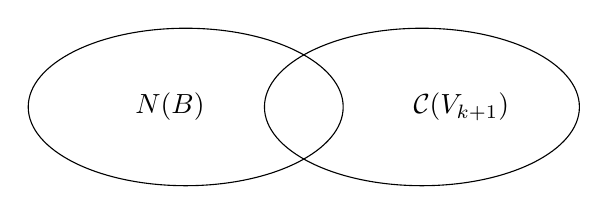
\begin{tikzpicture}
        \draw (0,0) ellipse (2cm and 1cm);
        \draw node at (-0.2,0) {$N(B)$};
        \draw (3,0) ellipse (2cm and 1cm);
        \draw node at (3.5,0) {$\mathcal{C}(V_{k+1})$};
    \end{tikzpicture}
\end{center}
Consider $\underline{w} \in N(B) \bigcap \mathcal{C}(V_{k+1})$, we suppose for easyness that $||\underline{w}||_2 = 1$.
\[
    \underline{w} = \sum_{i=1}^{k+1} c_i \underline{v_i} \overset{(\star)}{=} V_{k+1}\underline{c} \hspace{1cm} \sum_{i=1}^{k+1} c_i^2 = 1   
\]
We want to measure the following quantity:
\[
    ||A - B||^2_2 =  \underbrace{\underset{||\underline{v}||^2=1}{\sup} ||(A-B)\underline{w}||_2^2}_{\text{particular $||\underline{v}||$}} \geq \underbrace{||(A-B)\underline{w}||_2^2}_{\text{generic $||\underline{w}||$}} \implies
\]
Recall that $\underline{w} \in N(B) \implies B\underline{w} = 0$.
\[
    \implies ||A-B||^2_2 \geq ||A\underline{w}||_2^2 = \underline{w}^\intercal A^\intercal A \underline{w} \overset{\text{SVD}}{=} \underline{w}^\intercal V\Sigma^\intercal \underbrace{U^\intercal U}_{I} \Sigma V^\intercal  \underline{w} = 
\] 
\[
     \underline{w}^\intercal V\Sigma^\intercal \Sigma V^\intercal \underline{w} \overset{(\star)}{=} \underline{c}^\intercal \underbrace{V_{k+1}^\intercal V}_{I_{k+1}} \Sigma^\intercal \Sigma  \underbrace{V^\intercal V_{k+1}}_{I_{k+1}} \underline{c} = \underline{c}^\intercal \Sigma^\intercal \Sigma \underline{c} = \sum_{i=1}^{k+1} c_i^2 \sigma_i^2 \geq    
\] 
Since singular values are ordered
\[
    \geq \sigma_{k+1}^2 \underbrace{\sum_{i=1}^{k+1} c_i^2} = \sigma_{k+1}^2    
\]
So
\[
    ||A-B||_2^2 \geq \sigma_{k+1}^2 = ||A - A_k||_2^2    
\]
And, erasing the squares:
\[
    ||A - B||_2^2 \geq \sigma_{k+1} = ||A - A_k||_2        
\]
Where $A_k$ is the rank $k$ truncated SVD approximation, therefore
\[
    ||A - A_k||_2 \leq ||A - B||_2 \hspace{1cm} \forall B \text{ of rank } k
\]





\section{PCA}
Here is a first real-world application of the SVD. PCA has the same aim as SVD i.e. find a way of projecting the dataset in a new space where variances are maximized and covariances are minimized. 

We start from $A \in \mathbb{R}^{n \times d}$ and we follow these points:
\begin{enumerate}[i]
    \item \textbf{Center the matrix \emph{A}}\\
    $\bar{A}$ is the mean centered with respect to columns while $H$ is called the centering matrix and is obtained as follows:
    \[
        H = I_n - \dfrac{1}{n} \underline{\mathbbm{1}}_n \underline{\mathbbm{1}}_n^\intercal
    \]
    Where $\underline{\mathbbm{1}}_n$ is the vector of dimension $n$ containing all ones. The centered matrix is obtained:
    \[
        \bar{A} = HA    
    \]
    \item Build the covariance matrix
    \[
        S = \dfrac{\bar{A}^\intercal \bar{A}}{n - 1}     
    \]
    Where the denominator is $n-1$ is because we want an unbiased estimator and it's not $n$ because we have already taken 1 degree of freedom by centering the matrix. The covariance matrix is semidefinite positive so we can use eigenvalues and eigenvectors decomposition.
    \[
        SV = VD \implies VDV^\intercal, D = V^\intercal SV    
    \]
    If you order the eigenvalues in decreasing order the corresponding eigenvectors are called principal components. To notice the relationship between SVD and PCA we can write:
    \[
        S = \dfrac{1}{n-1}\bar{A}^\intercal \bar{A} = \dfrac{1}{n-1} V\Sigma^\intercal U^\intercal U \Sigma V^\intercal = \dfrac{1}{n-1} V \Sigma^2 V^\intercal    
    \]
    \[
        D = \dfrac{1}{n-1}\Sigma^2 \implies \lambda_k =\dfrac{\sigma_k^2}{n-1}    
    \]
\end{enumerate}
PCA is SVD applied to a particular matrix.


\subsection*{Choose rank of truncated SVD}
When using truncated SVD, how to choose the rank $k$? One possibility is to use $k$ such that a predefined percentage of the variance is retained. Another idea starts from:
\[
    A = A_{true} + \gamma A_{noise}    
\]
Where: 
\begin{itemize}
    \item $A$: is out dataset
    \item $A_{true}$: is the underlying low-rank representation of our data
    \item $\gamma$: magnitude of the noise
    \item $A_{noise}$: is a gaussian noise with 0 mean and unitary variance
\end{itemize}
By defining $\tau$ as threshold we have that if $sigma_i > \tau$ we are picking $A_{true}$. 
There are two cases:
\begin{itemize}
    \item $\gamma$ is known, i.e. we know the magnitude of the noise:
    \begin{itemize}
        \item if $A \in \mathbb{R}^{n \times n}$ (square) then $\tau = \dfrac{4}{\sqrt{3}}\gamma \sqrt{n}$
        \item if $A \in \mathbb{R}^{m \times n}$ we have two more cases:
        \begin{itemize}
            \item if $n \ll m \implies \tau = \lambda(\beta)$ where $\beta = \dfrac{n}{m}$ and $\lambda$ is the following function:
            \[
                \lambda(\beta) = \sqrt{2(\beta + 1) + \dfrac{8\beta}{(\beta+1)+\sqrt{(\beta^2 + 14\beta + 1))}}}    
            \]
            \item if $m \ll n \implies \tau = \lambda(\beta)$ where $\beta = \dfrac{m}{n}$ so it's equal as before but in this case the numerator and denumerator of $\beta$ are swapped.
        \end{itemize}
    \end{itemize}
    \item $\gamma$ is unknown. We define $\tau$ as follows:
    \[
        \tau = \omega(\beta)\sigma_{med} \hspace{1cm} \omega(\beta) = \dfrac{\lambda(\beta)}{\mu_{\beta}}    
    \]
    In which $\sigma_{med}$ is the median of the singular values and $\mu_{\beta}$ is the median of the Marcenko-Pastur distribution. $\lambda(\beta)$ is the same function as before. In particular:
    \[
        \mu_{\beta} = \int_{(1-\beta)^2}^{\mu_{\beta}} \dfrac{\sqrt{((1- \sqrt{\beta})^2 - t)(t - (1- \sqrt{\beta})^2)}}{2\pi t} dt = \dfrac{1}{2}    
    \]
\end{itemize}

\subsection*{Randomized SVD}

Randomized SVD is a faster and more efficient way to compute the truncated SVD, especially for large matrices. The key idea is to project the original matrix onto a lower-dimensional subspace using a random matrix, and then perform the SVD on the reduced matrix. The steps are as follows:

\begin{enumerate}

    \item Given an input matrix $A \in \mathbb{R}^{m \times n}$ and a target rank $k$, generate a random matrix $\Omega \in \mathbb{R}^{n \times k}$ whose entries are independent and identically distributed Gaussian random variables with zero mean and unit variance.

    

    \item Compute the matrix product $Y = A\Omega \in \mathbb{R}^{m \times k}$, which projects the columns of $A$ onto a $k$-dimensional subspace.

    

    \item Compute the QR decomposition of $Y$: $Y = QR$, where $Q \in \mathbb{R}^{m \times k}$ has orthonormal columns and $R \in \mathbb{R}^{k \times k}$ is upper triangular.

    

    \item Form the matrix $B = Q^T A \in \mathbb{R}^{k \times n}$, which is a low-rank approximation of $A$.

    

    \item Compute the SVD of the small matrix $B$: $B = \tilde{U} \Sigma V^T$, where $\tilde{U} \in \mathbb{R}^{k \times k}$, $\Sigma \in \mathbb{R}^{k \times k}$, and $V \in \mathbb{R}^{n \times k}$.

    

    \item Form the matrix $U = Q\tilde{U} \in \mathbb{R}^{m \times k}$, which contains the left singular vectors of $A$.

\end{enumerate}

The resulting matrices $U$, $\Sigma$, and $V$ form a rank-$k$ approximation of the SVD of $A$: $A \approx U\Sigma V^T$. The approximation error depends on the choice of the target rank $k$ and the quality of the random projection. In practice, the error can be controlled by oversampling, i.e., choosing a larger value for $k$ and then truncating the SVD to the desired rank.

The main advantage of randomized SVD is its computational efficiency. The algorithm requires only a few passes over the input matrix $A$ and avoids the expensive computation of the full SVD. This makes it particularly well-suited for large-scale problems where the full SVD is infeasible or prohibitively expensive.
\section{Least Squares Approximation}
Consider the following setup with $n > p$:
\begin{itemize}
    \item $X \in \mathbb{R}^{n \times p}$: feature matrix with $n$ samples and $p$ features, where $\text{rank}(X) = p$
    \item $\underline{y} \in \mathbb{R}^n$: label vector for each sample
\end{itemize}
The feature matrix $X$ can be written as:
\[
X = 
\begin{bmatrix}
    \horzbar & \underline{x_1^\intercal} & \horzbar\\
    \horzbar & \underline{x_2^\intercal} & \horzbar\\    
     & \vdots & \\
    \horzbar & \underline{x_n^\intercal} & \horzbar
\end{bmatrix}
\]
where $\underline{x_j}$ is the $j$-th column of $X$.

Given a new sample $\tilde{\underline{x}}$, we aim to predict its corresponding label $\tilde{y}$ using the information from the training set. We can use a linear model:
\[
    \tilde{y} = \tilde{\underline{x}}^\intercal \underline{w}, \quad \underline{w} \in \mathbb{R}^p
\]

Since $\underline{y} \neq X\underline{w}$ in general, we use the approximation $\hat{\underline{y}} = X\underline{w}$. Thus, $\hat{\underline{y}} \in \mathcal{C}(X)$, while $\underline{y} \notin \mathcal{C}(X)$ in general.

The prediction error for the $i$-th sample is given by:
\[
    r_i(\underline{w}) = \underline{y_i} - \underline{\hat{y_i}}    
\]
The goal is to minimize the squared $\ell_2$-norm of the residual vector $\underline{r}(\underline{w})$:
\[
    \hat{\underline{w}} = \underset{\underline{w}}{\arg\min}\,||\underline{r}(\underline{w})||^2_2
\]
There are two approaches to solve this problem:
\begin{enumerate}
    \item Geometrical interpretation
    \item Optimization procedures
\end{enumerate}

\subsection*{Geometrical Interpretation}
\begin{center} 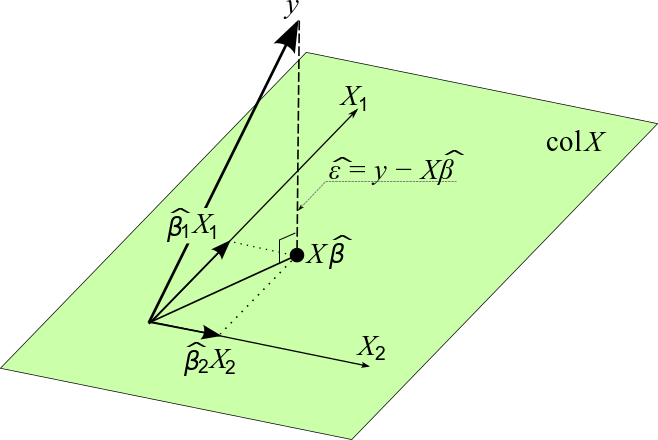
\includegraphics[scale = 0.4]{../images/OLS_geometric_interpretation.png} \end{center}
\begin{itemize}
    \item The plane represents the space of predictions $\mathcal{C}(X)$, spanned by the column vectors of $X$.
    \item $\underline{y}$ is the label vector to be predicted.
    \item $\hat{\underline{y}} = X\hat{\beta}$ is the projection of $\underline{y}$ onto $\mathcal{C}(X)$.
    \item $\underline{r}(\underline{w}) = \epsilon$ is the residual vector, representing the error between the predicted and actual labels.
\end{itemize}
For any $\underline{\overline{y}} \in \mathcal{C}(X)$ different from $\hat{\underline{y}}$, with residuals $\underline{\overline{r}} = \underline{y} - \underline{\overline{y}}$ and $\underline{\hat{r}} = \underline{y} - \underline{\hat{y}}$, we have:
\[
    ||\underline{\hat{r}}||_2 \leq ||\underline{\overline{r}}||_2
\]
This is because $\underline{\hat{r}}$ is the orthogonal projection of $\underline{y}$ onto $\mathcal{C}(X)$, and the orthogonal projection is the closest point to $\underline{y}$ in the subspace $\mathcal{C}(X)$.

Consequently, we have:
\[
    \underline{x_j^\intercal}\underline{\hat{r}} = 0, \quad j = 1, \dots, p    
\]
The residual vector $\underline{\hat{r}}$ is orthogonal to each column vector of the feature matrix $X$, meaning it is perpendicular to the subspace spanned by the columns of $X$.
In matrix form:
\[
    X^\intercal \underline{\hat{r}} = \underline{0} \implies X^\intercal (\underline{y} - \underline{\hat{y}}) = \underline{0} \implies X^\intercal (\underline{y} - X\underline{\hat{w}}) = \underline{0} \implies X^\intercal \underline{y} = X^\intercal X \underline{\hat{w}}
\]
If $X$ is full rank, then $X^\intercal X$ is also full rank and invertible. Thus, we can find $\hat{\underline{w}}$ as:
\[
    \hat{\underline{w}} = (X^\intercal X)^{-1}X^\intercal \underline{y}
\]


\subsection*{Optimization Perspective}
We can solve the problem using optimization techniques:
\[
    \hat{\underline{w}} = \underset{\underline{w}}{\arg\min}||\underline{r}(\underline{w})||^2_2 = \underset{\underline{w}}{\arg\min}||\underline{y} - X\underline{w}||^2_2 = \underset{\underline{w}}{\arg\min}(\underline{y} - X\underline{w})^\intercal(\underline{y} - X\underline{w})
\]
\[
    = \underset{\underline{w}}{\arg\min} \bigg[\underline{y}^\intercal \underline{y} - 2\underline{y}^\intercal X\underline{w} + \underline{w}^\intercal X^\intercal X\underline{w}\bigg] = \underset{\underline{w}}{\arg\min} F(\underline{w})
\]
$F(\underline{w})$ is a quadratic functional. If $X$ is full rank, then $X^\intercal X$ is positive definite, implying that the functional is strictly convex and has a unique minimum.

Setting the gradient to zero:
\[
    \nabla_{\underline{w}}F(\underline{w}) = -2X^\intercal \underline{y} + 2X^\intercal X\underline{w} = \underline{0}
\]
leads to the same solution as the geometrical interpretation.


We have obtained:
\[
    \underline{\hat{w}} = (X^\intercal X)^{-1} X^\intercal \underline{y} \implies \underline{\hat{y}} = \underbrace{X(X^\intercal X)^{-1} X^\intercal}_{P_x} \underline{y}     
\]
The matrix $P_x$ dimension is given by the product of: $(n\times p)(p\times p)(p \times n) = (n\times n)$ and has this properties:
\begin{itemize}
    \item $P_x = P_x^2$
    \item $P_x$ is a projection matrix
\end{itemize}

Let's consider $U$ an orthogonal ($U^\intercal U = I$) matrix that contains the basis for $\mathcal{C}(X)$ this means that $\mathcal{C}(X) = \mathcal{C}(U)$. We can write:
\[
    \underline{\hat{y}} = X\underline{\hat{w}} = U\underline{\tilde{w}}    
\]
So this basically means that the predicted value of $y$ still a projection on a plane but this time the plane is spanned by the columns of $U$ and not by the columns of $X$. By substituting last equation in the minimization method for least squares we have:
\[
    \underline{\tilde{w}} = \underset{\underline{w}}{\arg\min} ||\underline{y} - U\underline{w}||^2_2 \implies \underline{\hat{y}} = U\underline{\tilde{w}} = U(U^\intercal U)^{-1}U^\intercal \underline{y} = UU^\intercal \underline{y} 
\]
This formulation is possible because this time in the parenthesis we have an orthogonal matrix and this means that $(U^\intercal U)^{-1} = U^\intercal U = I$. In general $UU^\intercal \neq I$ because it might be rectangular (while $U^\intercal U$ is always square).\\







\subsection*{Ridge regression }
This method will help us in preventing the problem mentioned just before. We start from the definition of the weight vector for linear model explicited for the optimization method of the Least Squares:
\[
    \underline{\hat{w}}_{LS} = \arg \min_{\underline{w}} \underbrace{||\underline{y} - X\underline{w}||_2^2 + \lambda ||\underline{w}||_2^2}_{f(\underline{w})}
\]
In particular we have added a term. 
\[
    f(\underline{w}) = \underline{y}^\intercal \underline{y} - 2\underline{w}^\intercal X \underline{y} + \underline{w}^\intercal X^\intercal X \underline{w} + \lambda \underline{w}^\intercal \underline{w}
\]
We can now compute the gradient of this function:
\[
        \nabla_w(f(\underline{w})) = -2X^\intercal \underline{y} + 2X^\intercal X \underline{w} + 2\lambda \underline{w} = 0      
\]
\[
    X^\intercal \underline{y} = (X^\intercal X + \lambda I)\underline{w}     
\]
\[
    \underline{\hat{w}}_{R} = (X^\intercal X + \lambda I)^{-1} X^\intercal \underline{y}    
\]
It's easy to notice that if $\lambda = 0$ we get the Least Squares solution. If $\lambda > 0$ we will have a different solution. We can now compute the SVD of $X$:
\[
    \begin{split}
        \underline{\hat{w}}_R &= (V\Sigma^\intercal \underbrace{U^\intercal U}_{I} \Sigma V^\intercal + \lambda \underbrace{V V^\intercal}_{I})^{-1} V\Sigma^\intercal U^\intercal \underline{y} \\
        &= \left[V(\Sigma^\intercal \Sigma + \lambda I)V^\intercal\right]^{-1} V\Sigma^\intercal U^\intercal \underline{y} \\
        &= V\underbrace{(\Sigma^\intercal \Sigma + \lambda I) ^{-1}\Sigma^\intercal}_{M}U^\intercal \underline{y} \\
    \end{split}    
\]
Where 
\[
M = \begin{bmatrix}
    \dfrac{\sigma_1}{\sigma_1^2 + \lambda} & 0 & \dots & 0 & 0 & \dots & 0\\
    0 & \dfrac{\sigma_2}{\sigma_2^2 + \lambda} & \dots & 0 & 0 & \dots & 0\\
    \vdots & \vdots & \ddots & \vdots & \vdots & \ddots & \vdots\\
    0 & 0 & \dots & \dfrac{\sigma_p}{\sigma_p^2 + \lambda} & 0 & \dots & 0
\end{bmatrix}
\]
\begin{itemize}
    \item if $\sigma_i$ is big compared to $\lambda$ then $\dfrac{\sigma_i}{\sigma_i^2 + \lambda} \approx \dfrac{1}{\sigma_i}$
    \item if $\sigma_i$ is close to 0 then $\dfrac{\sigma_i}{\sigma_i^2 + \lambda} \approx 0$
\end{itemize}
Ridge regression addresses the problem of singular values close to zero in the matrix $X$ by adding a regularization term $\lambda$ to the diagonal of $X^\intercal X$. This modifies the singular values in the pseudo-inverse term to $\frac{\sigma_i}{\sigma_i^2 + \lambda}$. When $\sigma_i$ is much larger than $\lambda$, the solution remains similar to the Least Squares solution. However, when $\sigma_i$ is close to zero, the corresponding term in the pseudo-inverse becomes approximately zero, mitigating the issues caused by small singular values. As $\lambda$ approaches zero, the Ridge regression solution converges to the Least Squares solution. The choice of $\lambda$ depends on the desired balance between fitting the training data and regularizing the model, and is often selected using techniques like cross-validation.
If $\lambda$ is very small the matrix of $\Sigma$'s is almost equal to $\Sigma^+$.
\[
    \begin{split}
        \underline{\hat{w}}_R &= (X^\intercal X + \lambda I)^{-1} X^\intercal \underline{y}\\
        &= (X^\intercal X + \lambda I)^{-1} X^\intercal(X\underline{w}^* + \underline{\epsilon})\\
        &= (X^\intercal X + \lambda I)^{-1} X^\intercal X\underline{w}^* + (X^\intercal X + \lambda I)^{-1} X^\intercal \underline{\epsilon}\\
    \end{split}    
\]

\include{Lecture6}

\newpage

\subsection*{Orthogonal Least Squares}
In the last lecture we have introduced the least squares method. In particular we have mentioned the linear model for which:

$$
\underline{\hat{y}}=X \underline{\hat{w}} \quad X \in \mathbb{R}^{n \times p} \quad \underline{\hat{y}} \in \mathbb{R}^{n} \quad n \geq p \quad X \text { full rank }
$$

We have obtained:

$$
\underline{\hat{w}}=\left(X^{\top} X\right)^{-1} X^{\top} \underline{y} \Longrightarrow \underline{\hat{y}}=\underbrace{X\left(X^{\top} X\right)^{-1} X^{\top}}_{P_{x}} \underline{y}
$$

The matrix $P_{x}$ dimension is given by the product of: $(n \times p)(p \times p)(p \times n)=(n \times n)$ and has this properties:
- $P_{x}=P_{x}^{2}$
- $P_{x}$ is a projection matrix

Let's consider $U$ an orthogonal $\left(U^{\top} U=I\right)$ matrix that contains the basis for $\mathcal{C}(X)$ this means that $\mathcal{C}(X)=\mathcal{C}(U)$. We can write:

$$
\underline{\hat{y}}=X \underline{\hat{w}}=U \underline{\tilde{w}}
$$

So this basically means that the predicted value of $y$ still a projection on a plane but this time the plane is spanned by the columns of $U$ and not by the columns of $X$. By substituting last equation in the minimization method for least squares we have:

$$
\underline{\tilde{w}}=\underset{\underline{w}}{\arg \min }\|\underline{y}-U \underline{w}\|_{2}^{2} \Longrightarrow \underline{\hat{y}}=U \underline{\tilde{w}}=U\left(U^{\top} U\right)^{-1} U^{\top} \underline{y}=U U^{\top} \underline{y}
$$

This formulation is possible because this time in the parenthesis we have an orthogonal matrix and this means that $\left(U^{\top} U\right)^{-1}=U^{\top} U=I$. In general $U U^{\top} \neq I$ because it might be rectangular (while $U^{\top} U$ is always square).\\ 
How do we build the orthogonal matrix $U$ ? We can use the Gram-Schmidt procedure, but a drawback of Gram Schmidt is that, depending on the order chosen for the columns of $X$, the matrix $U$ can be different. Moreover, the order of vector columns of $U$ is meaningless.\\
Now, we want to exploit the SVD for computing the orthogonal matrix $U$. We start from the SVD of $X$ :


$$
\begin{aligned}
\underline{\hat{w}} & =\left(X^{\top} X\right)^{-1} X^{\top} y \\
& =\left(V \Sigma^{\top} U^{\top} U \Sigma V^{\top}\right)^{-1} V \Sigma^{\top} U^{\top} \underline{y} \\
& =\left(V \Sigma^{\top} \Sigma V^{\top}\right)^{-1} V \Sigma^{\top} U^{\top} \underline{y} \\
& =V\left(\Sigma^{\top} \Sigma\right)^{-1} \underbrace{V^{\top} V}_{I} \Sigma^{\top} U^{\top} \underline{y} \\
& = V\underbrace{\left(\Sigma^{\top} \Sigma\right)^{-1} \Sigma^{\top}}_{\Sigma^{+}} U^{\top} \underline{y} \\
& = V\Sigma^{+} U^{\top} \underline{y} \\
& = X^{+}\underline{y}
\end{aligned}
$$


$\Sigma^{+}$il called the pseudo-inverse of $\Sigma$.

Eventually, we have:


\\
Let's consider now the case in which \( p \geq n \) and \( X \) has \( n \) linearly independent rows (before we had \( p \) linearly independent columns). This means that we have more unknowns than equations and we would find infinite solutions for \(\underline{\hat{w}}\) such that \(\underline{\hat{y}} = X \underline{\hat{w}}\).

The solution found before, \(\underline{\hat{w}} = V \Sigma^{+} U^{\top} \underline{y}\), is still valid, but now \(\Sigma^{+} = \Sigma^{\top} (\Sigma \Sigma^{\top})^{-1}\). This means it has the same shape as before but transposed. \\ \\
Let's consider two vectors: w_\underline{w} and ˆw_\underline{\hat{w}}:

\[
\underline{y} = X \underline{w} = X \underline{\hat{w}}
\]

So they both are solutions of the system of equations.

To prove that the vector \(\underline{\hat{w}} = V \Sigma^{+} U^{\top} \underline{y}\) is the solution with the minimum norm among all solutions \(\underline{w}\) of the system \(\underline{y} = X \underline{w}\), we will use the properties of the SVD and the orthogonality of the matrices \(U\) and \(V\).\\ \\
We have that among the infinite solution, the one obtained through the psudo inverse is the on with minimal norm. \\
\begin{theorem}
For an underdetermined system $\underline{y} = X\underline{w}$, the solution $\hat{w}$ computed through the pseudoinverse has the minimum norm among all solutions.
\end{theorem}

\begin{proof}
Let $w$ be any solution to the underdetermined system, and $\hat{w}$ be the solution computed through the pseudoinverse. We will show that $\|\hat{w}\|_2^2 \leq \|w\|_2^2$.

We begin by expanding $\|w\|_2^2$:

\begin{align*}
\|w\|_2^2 &= \|w-\hat{w}+\hat{w}\|_2^2 \\
&= (w-\hat{w}+\hat{w})^{\top}(w-\hat{w}+\hat{w}) \\
&= (w-\hat{w})^{\top}(w-\hat{w}) + \hat{w}^{\top}\hat{w}li + 2(w-\hat{w})^{\top}\hat{w}
\end{align*}

Now, we use the following properties:

\begin{enumerate}
\item Both $w$ and $\hat{w}$ are solutions, so $Xw = X\hat{w} = y$. This implies $X(w - \hat{w}) = 0$, meaning $(w - \hat{w})$ is in the null space of $X$.\\

\item $\hat{w}$, being the pseudoinverse solution, is orthogonal to the null space of $X$. Therefore, $(w - \hat{w})^{\top}\hat{w} = 0$.\\
\end{enumerate}

Using these properties, we can simplify our expansion:

\begin{align*}
\|w\|_2^2 &= (w-\hat{w})^{\top}(w-\hat{w}) + \hat{w}^{\top}w + 2(w-\hat{w})^{\top}\hat{w} \\
&= (w-\hat{w})^{\top}(w-\hat{w}) + \hat{w}^{\top}\hat{w} + 0 \\
&= \|w-\hat{w}\|_2^2 + \|\hat{w}\|_2^2
\end{align*}

Since $\|w-\hat{w}\|_2^2$ is always non-negative, we can conclude that:

\begin{equation*}
\|w\|_2^2 \geq \|\hat{w}\|_2^2
\end{equation*}

This inequality holds for any solution $w$. Therefore, $\hat{w}$ has the minimum norm among all solutions of the system $\underline{y} = X\underline{w}$.
\end{proof}

\newpage

\section{Matrix completion}
We start from 
\[
    X \in \mathbb{R}^{n \times p}  \hspace{0.5cm} rank(X) = r \ll \min(n,p) 
\]
We know only partially X, we know $X_{i,j} \texttt{for} (i,j)\in\Omega(i,j) \in \Omega.$ 

Matrix completion is a method for filling missing values. If we had full rank matrix we would have independent columns so we would not be able to retrieve/obtain missing values. Being low rank, in this sense, helps us accomplishing this goal.  

\subsection*{Ideal estimator}
\[
    \begin{cases}
        \hat{X} = \underset{z \in \mathbb{R}^{n \times p}}{\arg \min} \left[\text{ rank}(z)\right]\\
        \text{subject to } \hat{X_{ij}} = X_{ij} (i,j) \in \Omega
    \end{cases}    
\]
This formulation is computationally unfeasible as  the object function is non-convex. Amongst all possible solutions, we are searching for the one with minimal rank.
The problem is that this is a non-convex optimization problem which requires a lot of computational power to be solved.

\subsection*{Practical estimator}
We are going to use the \textbf{Nuclear norm}: $||\cdot||_*  = \sum\limits_{i=1}^{\min(n,p)}\sigma_i$.

The idea is that, instead of minimizing the rank, we minimize the norm since, when performing the SVD, the number of non-zero singular values is equal to the rank of the matrix.
\[
    \begin{cases}
        \hat{X} = \underset{z \in \mathbb{R}^{n \times p}}{\arg \min} ||z||_*\\
        \text{subject to } \hat{X_{ij}} = X_{ij} (i,j) \in \Omega
    \end{cases}    
\]
This new formulation is convex optimization problem. How are we going to solve this problem? With the \textbf{SVT (Singular Value Threshold)}. Here is the algorithm:
\begin{itemize}
    \item Initialize $\hat{X} = \texttt{zeros}(n,p)$
    \item Set $\hat{X}_{ij} = X_{ij} \texttt{ for } (i,j) \in \Omega$
    \item For $k = 1,2, \dots, N$  
    \begin{itemize}
        \item $\hat{X}_{old} = \hat{X}$
        \item $[U, \Sigma, V^\intercal] = \texttt{svd}(\hat{X})$
        \item $\Sigma \rightarrow \hat{\Sigma} \hspace{0.2cm} \begin{cases}
            \hat{\sigma}_i = \sigma_i & \text{ if } \sigma_i > \tau\\
            \hat{\sigma}_i = 0 & \text{ otherwise }
        \end{cases}$
        \item $\hat{X} = U\hat{\Sigma}V^\intercal$
        \item $\hat{X}_{ij} = X_{ij} \texttt{ for } (i,j) \in \Omega$
    \end{itemize}
    \item $||\hat{X} - X_{old}|| < \epsilon$
\end{itemize}
The constant $\tau$ is imposing some sort of thresholding on the acceptance of singular values. This is an example of non-monothone algorithm because after the reduction of rank with the condition on sigmas, we override some value of the matrix to the one contained in $\Omega$. Is it proved that for a large enough index $k$ the algorithm converge to the solution. 
\section{Page Rank}
Consider four websites where the directed links between them represent navigational paths from one website to another. The interaction of these websites can be visualized through a directed graph as follows:

\begin{multicols}{2}
\begin{center}
    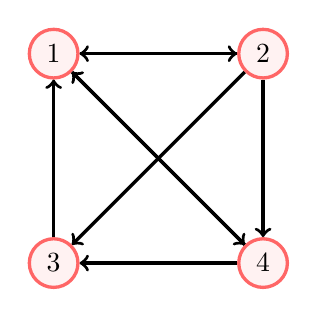
\begin{tikzpicture}[
    SIR/.style={circle, draw=red!60, fill=red!5, very thick, minimum size=5mm},
    node distance=2cm
    ]
    %Nodes
    \node[SIR]    (1)                              {1};
    \node[SIR]    (2)       [right=of 1] {2};
    \node[SIR]    (3)       [below=of 1] {3};
    \node[SIR]    (4)       [right=of 3] {4};
    
    %Lines
    \draw[->, very thick] (1) -> (2);
    \draw[->, very thick] (1) -> (4);
    \draw[->, very thick] (2) -> (4);
    \draw[->, very thick] (2) -> (1);
    \draw[->, very thick] (3) -> (1);
    \draw[->, very thick] (2) -> (3);
    \draw[->, very thick] (4) -> (3);
    \draw[->, very thick] (4) -> (1);
    \end{tikzpicture}
\end{center}

The process of web surfing can be described as a series of random walks on this graph, leading to a steady state where \(\pi_i\) represents the probability of being on the \(i\)-th website. The probability vector \(\underline{\pi} \in \mathbb{R}^4\) for four websites is as follows:
\end{multicols}

We represent the linkage of these websites with an \textbf{Adjacency Matrix}:
\[
    \tilde{A} = \begin{bmatrix}
        0 & 1 & 0 & 0\\
        1 & 0 & 1 & 1\\
        1 & 0 & 0 & 0\\
        1 & 0 & 1 & 0\\
    \end{bmatrix}
\]
\(\tilde{A}_{ij} = 1\) if there is a link from \(i\) to \(j\), and \(0\) otherwise. This matrix is then normalized so that each column sums to 1, resulting in:
\[
    A = \begin{bmatrix}
        0   & 1/3 & 1/2 & 1/2\\
        1/3 & 0   & 1/3 & 1/2\\
        1/3 & 0   & 0   & 0\\
        1/3 & 1/3 & 1/2 & 0\\
    \end{bmatrix}
\]

Multiplying this matrix \(A\) by the canonical basis vector \(\underline{e}_3 = \begin{bmatrix} 0 & 0 & 1 & 0 \end{bmatrix}^\intercal\) demonstrates the transition probabilities from the third website:
\[
    A\underline{e}_3 = \begin{bmatrix}
        1/2\\
        1/2\\
        0\\
        1/2\\
    \end{bmatrix}
\]

\subsection*{Steady State Analysis}
The steady state is reached when the state vector \(\underline{\pi}\) satisfies:
\[
    A\underline{\pi} = \underline{\pi}
\]
Here, \(\underline{\pi}\) is an eigenvector of \(A\) associated with the eigenvalue 1. Using the Perron-Frobenius theorem for positive matrices (matrices with all non-negative coefficients), we know the largest eigenvalue \(\lambda_1 = 1\).

\subsection*{Convergence via Power Method}
The power method is employed to compute the eigenvector associated to the biggest eigenvalue in absolute value. The algorithm proceeds as follows:
\begin{itemize}
    \item Start with \(\underline{\pi}^{(0)}\) normalized to 1.
    \item For \(k = 1, 2, \ldots\):
    \[
        \underline{\pi}^{(k)} = \frac{A\underline{\pi}^{(k-1)}}{||A\underline{\pi}^{(k-1)}||}
    \]
    \item Stop when \(\| \underline{\pi}^{(k)} - \underline{\pi}^{(k-1)} \| < \epsilon\).
\end{itemize}

As \(k \to \infty\), the method converges, isolating the principal eigenvector due to the dominance of \(\lambda_1\). This iterative process approximates \(\underline{\pi}\), estimating the long-term probabilities of visiting each website based on their interconnectedness. The closer the sub-dominant eigenvalues are to \(\lambda_1\), the slower the convergence.

This means that, the steady state is the eigenvector of the matrix $A$ with eigenvalue 1. The matrix $A$ is positive (not positive-definite) i.e. it has all non-negative cohefficients. A positive matrix is denoted with $A > 0$.
From Perron-Frobenius theory we know that $\lambda_1 = 1$ is the largest eigenvalue.
\[
    \lambda_1 = 1 > \lambda_2 > \lambda_3 > \dots > \lambda_n \hspace{1cm} \lambda_i \neq 0
\] 
As mentioned in a previous lecture, we can use the power method in order to retrieve the largest eigenvalue. In particular, we start from:
\[
    \underline{\pi}^{(0)} \hspace{0.5cm}\text{with}\hspace{0.5cm} ||\underline{\pi}^{(0)}||=1    
\]
Then, for $k = 1, 2, \dots $
\[
    \underline{\pi}^{(k)} = \dfrac{A\underline{\pi}^{(k-1)}}{||A\underline{\pi}^{(k-1)}||}    
\]
\[
    \text{if } ||\underline{\pi}^{(k)} - \underline{\pi}^{(k-1)}|| < \epsilon \text{ then stop}    
\]
Obviously, $\epsilon$ represents a tolerance value. As we can see, there is an recursive definition in a sense that, at each iteration, the same operation is made on the same variable. For example:
\[
    \underline{\pi}^{(1)} = \dfrac{A\underline{\pi}^{(0)}}{||A\underline{\pi}^{(0)}||}    
    \hspace{2cm}
    \underline{\pi}^{(2)} = \dfrac{A\underline{\pi}^{(1)}}{||A\underline{\pi}^{(1)}||} = \dfrac{A^2\underline{\pi}^{()}}{||A^2\underline{\pi}^{(k-1)}||} 
\]
So, iterating k times:
\[
    \underline{\pi}^{(k)} = \dfrac{A^k\underline{\pi}^{(0)}}{||A^k\underline{\pi}^{(0)}||}     
\]
Since in $A$ there are no columns that are completely equal to 0, the matrix can be diagonalized. This implies that there are some $\underline{v}_i, i = 1, \dots, n$ that can used as a basis for the space. In particular we can write:
\[
    \underline{\pi}^{(0)} = \sum_{i=1}^n \alpha_i \underline{v}_i
\]
We want to plug this expression in the previous equation (power method). Before, notice that, $A\underline{v}_i = \lambda \underline{v}_i$ because $\underline{v}_i$ are the vectors which diagonalize $A$ so the ones such that $A = V\Lambda V^\intercal$. 
The numerator of $\underline{\pi}^{(k)}$ can be written as:
\[
    A^k \underline{\pi}^{(0)} = \alpha_1\lambda_1^k \left(\underline{v}_1 + \sum_{i=2}^{n} \dfrac{\alpha_i}{\alpha_1}\left(\dfrac{\lambda_i}{\lambda_1}\right)^k \underline{v}_i\right)    
\]
\textbf{Proof:}
    \begin{align*}
                A^k \underline{\pi}^{(0)} &= V\Lambda^k V^{-1} \left(\alpha_1\underline{v}_1 + \dots + \alpha_n\underline{v}_n\right)\\
        &= V\Lambda^k \left(\alpha_1\underline{e}_1 + \dots + \alpha_n\underline{e}_n\right)\\
        &= V\left(\alpha_1\lambda_1^k\underline{e}_1 + \dots + \alpha_n\lambda_n^k\underline{e}_n \right)\\
        &=\alpha_1\lambda_1^k\underline{v}_1 + \dots + \alpha_n\lambda_n^k\underline{v}_n\\ 
        &= \alpha_1\lambda_1^k \left(\underline{v}_1 + \dfrac{\alpha_2}{\alpha_1}\left(\dfrac{\lambda_2}{\lambda_1}\right)^k \underline{v}_2 + \dots + \dfrac{\alpha_n}{\alpha_1}\left(\dfrac{\lambda_n}{\lambda_1}\right)^k \underline{v}_n\right)\\
\end{align*}


If $k \to \infty$ then $\left(\dfrac{\lambda_i}{\lambda_1}\right)^k \to 0$ because $\lambda_1 > \lambda_i$ for $i = 2, \dots, n$ . So, the only remaining term is $\underline{v}_1$ which is the eigenvector with the largest eigenvalue. So what we have just done is the proof of the convergence of the power method.The closer are the eigenvalues to $\lambda_1$ the slower is the convergence.   % lecture 8 absent because it was a lab
\section{Lasso Regression}
So far we have considered:
\[
    \underline{y} = X\underline{w} \hspace{1cm} X \in \mathbb{R}^{n \times p} \text{ and } \begin{Bmatrix}
        \text{Least Squares}: \underline{\hat{w}}_LS\\
        \text{Ridge Regression}: \underline{\hat{w}}_{RR}\\
    \end{Bmatrix} \underline{w} \in \mathbb{R}^p \text{ dense vector, i.e. not many zeros} 
\]
We are going to see a method which obtain a vector $\underline{\hat{w}}$ with many zeros, as sparse as possible. We want to consider this model:
\[
    \underline{y} = X\underline{w} \hspace{1cm} X \in \mathbb{R}^{n \times p} \hspace{1cm} p > n 
\]
We have said that the system is undetermined since it has infinite solutions. Suppose to have 2 features and 1 sample. 
\[
    X = \begin{bmatrix}
        2 & 3\\
    \end{bmatrix}
    \hspace{1cm}
    y = \begin{bmatrix}
        1\\
    \end{bmatrix}
\]
And so:
\[
    1 = \begin{bmatrix}
        2 & 3
    \end{bmatrix}\begin{bmatrix}
        w_1\\
        w_2
    \end{bmatrix} \implies
    1 = 2w_1 + 3w_2 \hspace{0.2cm} \leftarrow \hspace{0.2cm} \text{line}    
\]
As mentioned in a previous lecture, we want to find the minimum length solution so we can plot the line found before and the circles that represents the l2-norm distance.
\begin{center}
    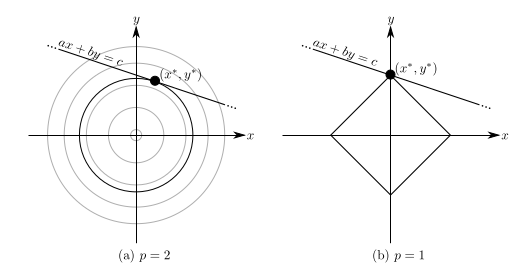
\includegraphics[scale=0.6]{../images/LassoRidgePlot.png}
\end{center}
On the right-hand side it is represented the equivalent plot but with the l1-norm. We can see that the solution on the right has one coordinate (are features!) that is equal to zero. This is true in general, i.e. we will obtain sparser solution using the l1-norm rather than the l2-norm.\\
With L1-norm it's still a convex optimization problem and
\[
    F(\underline{w}) = ||X\underline{w} - \underline{y}||_2^2 + \lambda ||\underline{w}||_1    
\] 
This model is implemented by \textbf{Lasso} (Least Absolute Shrinkage and Selection Operator) and achieve both the shortest distance solution and the selection of some features.

This is important because by reducing the number of features, we increase the interpretability of the model.\\

There is also the \textbf{Elastic Net} which combines both Lasso and Ridge: 
\[
    F(\underline{w}) = ||X\underline{w} - \underline{y}||_2^2 + \lambda_1||\underline{w}||_1 + \lambda_2||\underline{w}||_2^2  
\] 
\newpage
\section{Kernel Methods}

Kernel methods extend linear models to capture non-linear relationships without explicitly computing high-dimensional feature representations.

\subsection*{Feature Maps}

We start by transforming our original feature vector $x_\underline{x}$ using a feature map $\phi(x)$:
\[
    \phi(x) = \begin{bmatrix}
        x_1 \\ x_2 \\ x_1^2 \\ x_2^2 \\ x_1x_2
    \end{bmatrix} \in \mathbb{R}^d \quad (d > p \text{ typically})
\]

This leads to a new model representation:
\[
    \hat{y}_i = \phi(x_i)^\intercal \underline{w}
\]

\subsection*{The Kernel Trick}

To avoid computing large vectors, we introduce the kernel trick:
\[
    K(\underline{x}_i, \underline{x}_j) = \phi(\underline{x}_i)^\intercal \phi(\underline{x}_j)
\]

Common kernel functions include:
\begin{itemize}
    \item Polynomial of degree $q$: $K(\underline{x}_i, \underline{x}_j) = (\underline{x}_i^\intercal \underline{x}_j)^q$
    \item Polynomial of degree up to $q$: $K(\underline{x}_i, \underline{x}_j) = (\underline{x}_i^\intercal \underline{x}_j + 1)^q$
    \item Gaussian RBF: $K(\underline{x}_i, \underline{x}_j) = \exp(-\frac{||\underline{x}_i - \underline{x}_j||_2^2}{2\sigma^2})$
\end{itemize}

\subsection*{Kernel Ridge Regression}

In kernel ridge regression, we compute:
\[
    \underline{\alpha} = (K + \lambda I)^{-1} \underline{y}
\]
The matrix $K$ associated to Kernel has entries
\[ K_{i,j} = K(x_i, x_j) = \Phi(x_i)^T \Phi(x_j) \]

\[ \alpha = (\Phi^T \Phi + \lambda I)^{-1}  y = (K + \lambda I)^{-1} y \]

\[ y = w^T \Phi(x) = (\Phi^T \alpha)^T \Phi(x) = \alpha^T \Phi(x) \]
\[ = \sum_{i=1}^n \alpha_i (\Phi(x_i)^T \Phi(x)) \]
\[ = \sum_{i=1}^n \alpha_i K(x, x_i) \] % how far is the new sample from x_i

% contribution of sample i to the definition of decision boundary

\textbf{NB} notice that in this way, $\alpha$ can be computed without the feature map (costly), but only using the Kernel function (cheap!). 
$K$ could be singular, the term $\lambda I$ avoids the singular case
This technique is called \textit{Kernel trick}.


\subsection*{Representer Theorem}

Let $\hat{y}_i = w^T \Phi(x_i)$ with fixed feature map $\Phi$ and $w$ is learned from data $\{x_i, y_i\}$. Furthermore, let $L(y, \hat{y})$ be any loss function and $h: [0, +\infty) \rightarrow \mathbb{R}$ a strictly monotonically increasing function. Then each minimizer $w$ of
\[ \frac{1}{n} \sum_{i=1}^n L(y_i, w^T \Phi(x_i)) + h(\|w\|^2) \] % L2 regularization term
can be written as $w = \Phi^T \alpha$, where $\alpha$ is $n$-dimensional.

\textbf{NB:} A \textit{loss function} is a function that maps a single sample to a real number
\[ L(\phi, \hat{y}(x_i)) \]
then the \textit{cost function} concerns the entire sample set
\[ \frac{1}{n} \sum_{i=1}^n L(y_i, \hat{y}(x_i)) \]

\subsection*{Support Vector Regression}

Support Vector Regression (SVR) employs an $\epsilon$-insensitive loss function, which ignores errors within a certain threshold $\epsilon$. The loss function is defined as:
\[ 
L(y_i, \hat{y}) = \max(0, |y_i - \hat{y}| - \epsilon) 
\]
\[ 
= \begin{cases} 
0 & \text{if } |y_i - \hat{y}| \leq \epsilon, \\
|y_i - \hat{y}| - \epsilon & \text{otherwise.}
\end{cases} 
\]
Here, $\epsilon$ is a user-defined parameter that sets the width of the tube within which no penalty is given for errors.

The objective in SVR is to find the weight vector $w$ that minimizes the following primal formulation:
\[ 
\hat{w} = \arg\min_w \left\{ \frac{1}{n} \sum_{i=1}^n \max(0, |y_i - w^T \Phi(x_i)| - \epsilon) + \lambda \|w\|^2 \right\} 
\]
This formulation includes an $L_2$ regularization term controlled by $\lambda$, which helps prevent overfitting by penalizing the magnitude of the coefficients.

Although a direct dual formulation similar to the linear case is challenging to derive in the non-linear scenario, the dual problem in SVR can be formulated using kernel functions. The predicted value $\hat{y}(x)$ using the dual coefficients is expressed as:
\[ 
\hat{y}(\tilde{x}) = \hat{\alpha}^T K(X, \tilde{x}) 
\]
Where $K$ is the kernel function, encapsulating the inner product of vectors in a transformed feature space.

The dual coefficients $\alpha$ are obtained by solving:
\[ 
\hat{\alpha} = \arg\min_{\alpha} \frac{1}{2} \alpha^T K(X, X) \alpha - \alpha^T y + \epsilon \| \alpha \|_1 
\]
subject to the constraint $|\alpha_i| \leq \frac{1}{2n\lambda}$, which ensures that the solution does not overfit and that the influence of each data point is limited.




\section{Automatic Differentiation}

In this section, we will explore different methods for computing the derivative of a function:

\begin{center}
\begin{tabular}{|| m{14em} | m{12em} | m{20em} ||} 
 \hline
 Method & PROS & CONS \\ [0.5ex] 
 \hline\hline
 Manual computation & Exact, useful for proofs & Prone to error, time-consuming for complex functions\\ 
 \hline
 Numerical differentiation & Easy to program & Issues with floating point precision*, computationally expensive\\
 \hline
 Symbolic differentiation & Exact, good for proofs & Expression swelling**, cannot handle conditions or loops \\ 
 \hline
 Automatic differentiation (AD) & Exact, fast & Complex to implement \\ 
 \hline
\end{tabular}
\end{center}

\subsection*{Automatic Differentiation}

Automatic differentiation (AD) is a set of techniques to evaluate the derivative of a function specified by a computer program. Unlike symbolic differentiation, which manipulates mathematical expressions to find the derivative, and numerical differentiation, which approximates the derivative using finite differences, AD computes the derivative using the actual operations performed in the function, ensuring exact results up to machine precision.

AD exploits the fact that any program, no matter how complex, executes a sequence of elementary arithmetic operations (addition, subtraction, multiplication, division) and elementary functions (exp, log, sin, cos, etc.). By applying the chain rule of calculus repeatedly to these operations, AD computes the derivatives efficiently and accurately.



\section*{An Example}

Consider the following function of 3 variables:

$$
f(x)=\left(x_{1} x_{2} \sin x_{3}+e^{x_{1} x_{2}}\right) / x_{3}
$$

$$
\begin{aligned}
& x_{4}=x_{1} * x_{2} \\
& x_{5}=\sin x_{3} \\
& x_{6}=e^{x_{4}} \\
& x_{7}=x_{4} * x_{5} \\
& x_{8}=x_{6}+x_{7} \\
& x_{9}=x_{8} / x_{3}
\end{aligned}
$$



\section*{The Forward Mode}

\subsubsection*{An Overview}
Forward-mode autodiff is neither numerical differentiation nor symbolic differentiation, but in some ways, it is their love child. It relies on dual numbers, which are (weird but fascinating) numbers of the form \(a + b\epsilon\) where \(a\) and \(b\) are real numbers and \(\epsilon\) is an infinitesimal number such that \(\epsilon^2 = 0\) (but \(\epsilon \neq 0\)). You can think of the dual number \(42 + 24\epsilon\) as something akin to \(42.0000\ldots000024\) with an infinite number of 0s (but of course, this is simplified just to give you some idea of what dual numbers are). A dual number is represented in memory as a pair of floats. For example, \(42 + 24\epsilon\) is represented by the pair \((42.0, 24.0)\).

Dual numbers can be added, multiplied, and so on, as shown in the equations:
\[
\lambda (a + b\epsilon) = \lambda a + \lambda b\epsilon
\]
\[
(a + b\epsilon) + (c + d\epsilon) = (a + c) + (b + d)\epsilon
\]
\[
(a + b\epsilon) \times (c + d\epsilon) = ac + (ad + bc)\epsilon + bd\epsilon^2 = ac + (ad + bc)\epsilon
\]

Most importantly, it can be shown that \(h(a + b\epsilon) = h(a) + b \times h'(a)\epsilon\), so computing \(h(a + \epsilon)\) gives you both \(h(a)\) and the derivative \(h'(a)\) in just one shot. The computation of the partial derivative of \(f(x, y)\) with regards to \(x\) at \(x = 3\) and \(y = 4\) involves computing \(f(3 + \epsilon, 4)\); this will output a dual number whose first component is equal to \(f(3, 4)\) and whose second component is equal to \(\frac{\partial f}{\partial x}(3, 4)\).

To compute \(\frac{\partial f}{\partial y}(3, 4)\) we would have to go through the graph again, but this time with \(x = 3\) and \(y = 4 + \epsilon\).

So forward-mode autodiff is much more accurate than numerical differentiation, but it suffers from the same major flaw: if there were 1,000 parameters, it would require 1,000 passes through the graph to compute all the partial derivatives. This is where reverse-mode autodiff shines: it can compute all of them in just two passes through the graph.


\subsubsection*{More in detail}

In the forward mode of automatic differentiation, we evaluate and carry forward a directional derivative of each intermediate variable $x_{i}$ in a given direction $p \in \mathbb{R}^{n}$, simultaneously with the evaluation of $x_{i}$ itself. For the three-variable example above, we use the following notation for the directional derivative for $p$ associated with each variable:

$$
D_{p} x_{i} \stackrel{\text { def }}{=}\left(\nabla x_{i}\right)^{T} p=\sum_{j=1}^{3} \frac{\partial x_{i}}{\partial x_{j}} p_{j}, \quad i=1,2, \ldots, 9
$$

where $\nabla$ indicates the gradient with respect to the three independent variables. Our goal is to evaluate $D_{p} x_{9}$, which is the same as the directional derivative $\nabla f(x)^{T} p$. We note immediately that initial values $D_{p} x_{i}$ for the independent variables $x_{i}, i=1,2,3$, are simply the components $p_{1}, p_{2}, p_{3}$ of $p$. The direction $p$ is referred to as the seed vector.\\ \\
As soon as the value of $x_{i}$ at any node is known, we can find the corresponding value of $D_{p} x_{i}$ from the chain rule. For instance, suppose we know the values of $x_{4}, D_{p} x_{4}, x_{5}$, and $D_{p} x_{5}$, and we are about to calculate $x_{7}$. We have that $x_{7}=x_{4} x_{5}$; that is, $x_{7}$ is a function of the two variables $x_{4}$ and $x_{5}$, which in turn are functions of $x_{1}, x_{2}, x_{3}$. By applying the chain rule, we have that:
$$
\nabla x_{7}=\frac{\partial x_{7}}{\partial x_{4}} \nabla x_{4}+\frac{\partial x_{7}}{\partial x_{5}} \nabla x_{5}=x_{5} \nabla x_{4}+x_{4} \nabla x_{5}
$$

By taking the inner product of both sides of this expression with $p$ and applyingthe chain rule in the multivariate context we obtain:

$$
D_{p} x_{7}=\frac{\partial x_{7}}{\partial x_{4}} D_{p} x_{4}+\frac{\partial x_{7}}{\partial x_{5}} D_{p} x_{5}=x_{5} D_{p} x_{4}+x_{4} D_{p} x_{5}
$$\\
The directional derivatives $D_{p} x_{i}$ are therefore evaluated side by side with the intermediate results $x_{i}$, and at the end of the process we obtain $D_{p} x_{9}=D_{p} f=\nabla f(x)^{T} p$.\\ \\
The principle of the forward mode is straightforward enough, but what of its practical implementation and computational requirements? First, we repeat that the user does not need to construct the computational graph, break the computation down into elementary operations, or identify intermediate variables. The automatic differentiation software should perform these tasks implicitly and automatically. Nor is it necessary to store
the information $x_{i}$ and $D_{p} x_{i}$ for every node of the computation graph at once (which is just as well, since this graph can be very large for complicated functions). Once all the children of any node have been evaluated, its associated values $x_{i}$ and $D_{p} x_{i}$ are not needed further and may be overwritten in storage.\\ \\
The key to practical implementation is the side-by-side evaluation of $x_{i}$ and $D_{p} x_{i}$. The automatic differentiation software associates a scalar $D_{p} w$ with any scalar $w$ that appears in the evaluation code. Whenever $w$ is used in an arithmetic computation, the software performs an associated operation (based on the chain rule) with the gradient vector $D_{p} w$. For instance, if $w$ is combined in a division operation with another value $y$ to produce a new value $z$, that is,
$$
z \leftarrow \frac{w}{y}
$$

we use $w, z, D_{p} w$, and $D_{p} y$ to evaluate the directional derivative $D_{p} z$ as follows:

$$
D_{p} z \leftarrow \frac{1}{y} D_{p} w-\frac{w}{y^{2}} D_{p} y
$$

To obtain the complete gradient vector, we can carry out this procedure simultaneously for the $n$ seed vectors $p=e_{1}, e_{2}, \ldots, e_{n}$. We see that $p=e_{j}$ implies that $D_{p} f=\partial f / \partial x_{j}, j=1,2, \ldots, n$. We notethat the additional cost of evaluating $f$ and $\nabla f$ (over the cost of evaluating $f$ alone) may be significant. It is difficult to obtain an exact bound on the increase in computation, since the costs of retrieving and storing the data should also be taken into account. The storage requirements may also increase by a factor as large as $n$, since we now have to store $n$ additional scalars $D_{e_{j}} x_{i}, j=1,2, \ldots, n$, alongside each intermediate variable $x_{i}$. 

\section*{The Reverse Mode}

\subsection*{An Overview}
Reverse-mode autodiff is the solution implemented by TensorFlow. It first goes through the graph in the forward direction (i.e., from the inputs to the output) to compute the value of each node. Then it does a second pass, this time in the reverse direction (i.e., from the output to the inputs) to compute all the partial derivatives. During the first pass, all the node values were computed, starting from \(x = 3\) and \(y = 4\). You can see those values at the bottom right of each node (e.g., \(x \times x = 9\)). The nodes are labeled \(n_1\) to \(n_7\) for clarity. The output node is \(n_7: f(3,4) = n_7 = 42\).

The idea is to gradually go down the graph, computing the partial derivative of \(f(x,y)\) with regards to each consecutive node, until we reach the variable nodes. For this, reverse-mode autodiff relies heavily on the chain rule, shown in the equations:
\[
\frac{\partial f}{\partial x} = \frac{\partial f}{\partial n_i} \times \frac{\partial n_i}{\partial x}
\]
Since \(n_7\) is the output node, \(f = n_7\) so trivially \(\frac{\partial f}{\partial n_7} = 1\).

Let’s continue down the graph to \(n_5\): how much does \(f\) vary when \(n_5\) varies? The answer is:
\[
\frac{\partial f}{\partial n_5} = \frac{\partial f}{\partial n_7} \times \frac{\partial n_7}{\partial n_5}
\]
We already know that \(\frac{\partial f}{\partial n_7} = 1\), so all we need is \(\frac{\partial n_7}{\partial n_5}\). Since \(n_7\) simply performs the sum \(n_5 + n_6\), we find that:
\[
\frac{\partial n_7}{\partial n_5} = 1, \quad \frac{\partial f}{\partial n_5} = 1 \times 1 = 1
\]

Now we can proceed to node \(n_4\): how much does \(f\) vary when \(n_4\) varies? The answer is:
\[
\frac{\partial f}{\partial n_4} = \frac{\partial f}{\partial n_5} \times \frac{\partial n_5}{\partial n_4}
\]
Since \(n_5 = n_4 \times n_2\), we find that:
\[
\frac{\partial n_5}{\partial n_4} = n_2, \quad \frac{\partial f}{\partial n_4} = 1 \times n_2 = 4
\]

The process continues until we reach the bottom of the graph. At that point, we will have calculated all the partial derivatives of \(f(x,y)\) at the point \(x = 3\) and \(y = 4\). In this example, we find \(\frac{\partial f}{\partial x} = 24\) and \(\frac{\partial f}{\partial y} = 10\). Sounds about right!

Reverse-mode autodiff is a very powerful and accurate technique, especially when there are many inputs and few outputs, since it requires only one forward pass plus one reverse pass per output to compute all the partial derivatives for all outputs with regards to all the inputs. Most importantly, it can deal with functions defined by arbitrary code. It can also handle functions that are not entirely differentiable,


\subsection*{More in detail}

The reverse mode of automatic differentiation does not perform function and gradient evaluations concurrently. Instead, after the evaluation of $f$ is complete, it recovers the partial
derivatives of $f$ with respect to each variable $x_{i}$-independent and intermediate variables alike-by performing a reverse sweep of the computational graph. At the conclusion of this process, the gradient vector $\nabla f$ can be assembled from the partial derivatives $\partial f / \partial x_{i}$ with respect to the independent variables $x_{i}, i=1,2, \ldots, n$.

Instead of the gradient vectors $D_{p} x_{i}$ used in the forward mode, the reverse mode associates a scalar variable $\bar{x}_{i}$ with each node in the graph; information about the partial derivative $\partial f / \partial x_{i}$ is accumulated in $\bar{x}_{i}$ during the reverse sweep. The $\bar{x}_{i}$ are sometimes called the adjoint variables, and we initialize their values to zero, with the exception of the rightmost node in the graph (node $N$, say), for which we set $\bar{x}_{N}=1$. This choice makes sense because $x_{N}$ contains the final function value $f$, so we have $\partial f /$ $\partial x_{N}=1$.

The reverse sweep makes use of the following observation, which is again based on the chain rule: For any node $i$, the partial derivative $\partial f / \partial x_{i}$ can be built up from the partial derivatives $\partial f / \partial x_{j}$ corresponding to its child nodes $j$ according to the following formula:

$$
\frac{\partial f}{\partial x_{i}}=\sum_{j \text { a child of } i} \frac{\partial f}{\partial x_{j}} \frac{\partial x_{j}}{\partial x_{i}}
$$

For each node $i$, we add the right-hand-side term to $\bar{x}_{i}$ as soon as it becomes known; that is, we perform the operation

$$
\bar{x}_{i}+=\frac{\partial f}{\partial x_{j}} \frac{\partial x_{j}}{\partial x_{i}}
$$

(In this expression and the ones below, we use the arithmetic notation of the programming language $\mathrm{C}$, in which $x+=a$ means $x \leftarrow x+a$.) Once contributions have been received from all the child nodes of $i$, we have $\bar{x}_{i}=\partial f / \partial x_{i}$, so we declare node $i$ to be "finalized." At this point, node $i$ is ready to contribute a term to the summation for each of its parent nodes. The process continues in this fashion until all nodes are finalized. Note that for derivative evaluation, the flow of computation in the graph is from children to parents-the opposite direction to the computation flow for function evaluation.

During the reverse sweep, we work with numerical values, not with formulae or computer code involving the variables $x_{i}$ or the partial derivatives $\partial f / \partial x_{i}$. During the forward sweep-the evaluation of $f$-we not only calculate the values of each variable $x_{i}$, but we also calculate and store the numerical values of each partial derivative $\partial x_{j} / \partial x_{i}$. Each of these partial derivatives is associated with a particular arc of the computational graph. The numerical values of $\partial x_{j} / \partial x_{i}$ computed during the forward sweep are then used during the reverse sweep.




The main appeal of the reverse mode is that its computational complexity is low for the scalar functions $f: \mathbb{R}^{n} \rightarrow \mathbb{R}$ discussed here. The extra arithmetic associated with the gradient computation is at most four or five times the arithmetic needed to evaluate the function alone. \\
As we noted above, the forward mode may require up to $n$ times more arithmetic to compute the gradient $\nabla f$ than to compute the function $f$ alone, making it appear uncompetitive with the reverse mode. When we consider vector functions $r: \mathbb{R}^{n} \rightarrow \mathbb{R}^{m}$, the relative costs of the forward and reverse modes become more similar as $m$ increases, as we describe in the next section.\\
An apparent drawback of the reverse mode is the need to store the entire computational graph, which is needed for the reverse sweep. In principle, storage of this graph is not too difficult to implement. Whenever an elementary operation is performed, we can form and store a new node containing the intermediate result, pointers to the (one or two) parent nodes, and the partial derivatives associated with these arcs. During the reverse sweep, the nodes can be read in the reverse order to that in which they were written, giving a particularly simple access pattern. 
Unfortunately, the computational graph may require a huge amount of storage.



\subsection*{Matrix-Free Jacobian-Vector Product with Forward Mode Automatic Differentiation}

Forward mode automatic differentiation (AD) provides a very efficient and matrix-free way of computing Jacobian--vector products. This method utilizes the concept of a seed vector to guide the derivative computations. The seed vector \(\dot{\mathbf{x}}\) is initialized with \(\mathbf{r}\), defining the direction of differentiation right at the start:

\[
J_f \mathbf{r} = \begin{bmatrix}
    \frac{\partial y_1}{\partial x_1} & \cdots & \frac{\partial y_1}{\partial x_n} \\
    \vdots & \ddots & \vdots \\
    \frac{\partial y_m}{\partial x_1} & \cdots & \frac{\partial y_m}{\partial x_n} 
\end{bmatrix} \begin{bmatrix}
    r_1 \\
    \vdots \\
    r_n
\end{bmatrix},
\]

This approach enables the computation of the Jacobian--vector product in just one forward pass of the AD process by efficiently propagating changes along the direction specified by the seed vector \(\mathbf{r}\). As a special case, when \( f : \mathbb{R}^n \to \mathbb{R} \), we can obtain the directional derivative along a given vector \(\mathbf{r}\) as:

\[
\nabla f \cdot \mathbf{r}
\]

This is achieved by starting the AD computation with the values \(\dot{\mathbf{x}} = \mathbf{r}\), directly obtaining the rate of change of \(f\) in the direction of \(\mathbf{r}\). 


Forward mode AD is efficient and straightforward for functions $f : \mathbb{R} \to \mathbb{R}^m$, as all the derivatives $\frac{dy_i}{dx}$ can be computed with just one forward pass. Conversely, in the other extreme of $f : \mathbb{R}^n \to \mathbb{R}$, forward mode AD requires $n$ evaluations to compute the gradient
\[
\nabla f = \left(\frac{\partial y}{\partial x_1}, \dots, \frac{\partial y}{\partial x_n}\right),
\]
which also corresponds to a $1 \times n$ Jacobian matrix that is built one column at a time with the forward mode in $n$ evaluations.



\subsection*{Dual-numbers}
They are similar to complex numbers. 
\[
    a + b\epsilon \hspace{0.3cm} \text{ with }\hspace{0.3cm} a,b \in \mathbb{R} \hspace{0.3cm} \text{and} \hspace{0.3cm} \epsilon \neq 0, \epsilon^2 = 0    
\]
Where $a$ is the real part and $b$ is the dual part. Basic operations with dual numbers:
\[
    (a + b\epsilon) + (c + d\epsilon) = (a + c) + (b + d)\epsilon    
\]
\[
    (a + b\epsilon)(c + d\epsilon) = ac + (ad + bc)\epsilon     
\]
Why this algebra is useful to our purposes? Consider the generic function $f$, we want to evaluate it with a dual number:
\[
    f(a + b\epsilon) = f(a) + f'(a)b\epsilon + \underbrace{\dfrac{f''(a)}{2}b^2\epsilon^2   + \dots}_{0}
\]
We have used the Taylor expansion, the last terms are zero because of $\epsilon^2$. Notice that, if we have unitary dual part ($b = 1$), we obtain the derivative of $f$ in $a$. This is the key point of the dual numbers:
\[
    b=1 \implies a + b\epsilon = a + \epsilon \implies f(a + \epsilon) = f(a) + f'(a)\epsilon    
\]
The last term is again a dual number in which the real part is the value of the function in $a$ and the dual part is the derivative of the function in $a$.\\

Let's check if the derivative properties are actually respected, suppose to have $f(x) = g(x)h(x)$:
\[
    \begin{split}
        f(a + \epsilon) &= g(a + \epsilon)h(a + \epsilon)\\
        &= [g(a) + g'(a)\epsilon][h(a) + h'(a)\epsilon]\\
        &= g(a)h(a) + g(a)h'(a)\epsilon + g'(a)h(a)\epsilon + g'(a)h'(a)\epsilon^2\\
        &= g(a)h(a) + \underbrace{[g(a)h'(a) + g'(a)h(a)]}_{\text{der. of the product}}\epsilon\\
    \end{split}
\]
Or $f(x) = g(h(x))$:
\[
    \begin{split}
        f(a + \epsilon) &= g(h(a + \epsilon))\\
        &= g(h(a) + h'(a)\epsilon)\\
        &= \underbrace{ g(h(a))}_{f(a)} + \underbrace{g'(h(a))h'(a)\epsilon}_{f'(a)\epsilon}\\        
    \end{split}
\]


\subsection*{Usage of Automatic Differentiation}

Consider a function \( f: \mathbb{R}^n \to \mathbb{R} \). Automatic Differentiation (AD) can efficiently compute the Jacobian matrix \( \mathbf{J} \) using either Forward Mode (FM) or Backward Mode (BM). In FM, the operation count is approximately \( n \times c \times \operatorname{ops}(f) \), where \( c \approx 2.5 \). In BM, it is \( m \times c \times \operatorname{ops}(f) \), with \( m \) and \( n \) representing the dimensions of the output and input spaces, respectively. FM computes \( \mathbf{J}\underline{r} \) by setting \( \underline{\dot{x}} = \underline{r} \), which represents the product of the Jacobian with a vector. Conversely, BM computes \( \mathbf{J}^\top \underline{r} \) by setting \( \bar{\underline{y}} = \underline{r} \), which corresponds to the transpose Jacobian-vector product. BM necessitates storing all intermediate values from the forward computation for use during the backward computation.

We can also devise schemes based on the reverse mode for calculating Hessian-vector products \( \nabla^2 f(x)q \), or the full Hessian \( \nabla^2 f(x) \). A scheme for obtaining \( \nabla^2 f(x)q \) proceeds as follows. We start by using the forward mode to evaluate both \( f \) and \( \nabla f(x)^T q \), by accumulating the two variables \( x_i \) and \( D_q x_i \) during the forward sweep in the manner described above. We then apply the reverse mode in the normal fashion to the computed function \( \nabla f(x)^T q \). At the end of the reverse sweep, the nodes \( i = 1, 2, \ldots, n \) of the computational graph that correspond to the independent variables will contain
\[
\frac{\partial}{\partial x_i} (\nabla f(x)^T q) = [\nabla^2 f(x)q]_i, \quad i = 1, 2, \ldots, n.
\]


The number of arithmetic operations required to obtain \( \nabla^2 f(x)q \) by this procedure increases by only a modest factor, independent of \( n \), over the evaluation of \( f \) alone. By the usual analysis for the forward mode, we see that the computation of \( f \) and \( \nabla f(x)^T q \) jointly requires a small multiple of the operation count for \( f \) alone, while the reverse sweep introduces a further factor of at most 5. The total increase factor is approximately 12 over the operation count for \( f \) alone.

For more complex requirements, such as when the full Hessian \( \nabla^2 f(x) \) is needed or when \( \nabla^2 f(x) q \) must be computed, a combination of FM and BM is employed. The forward mode evaluates both \( f \) and \( \nabla f(x)^T q \), and the reverse mode subsequently computes \( \nabla^2 f(x) q \). This procedure increases the operation count by a factor of approximately 12 over the evaluation of \( f \) alone. Utilizing different seed vectors \( q \) (e.g., \( e_1, e_2, \ldots, e_n \) for the full Hessian) and possibly employing graph-coloring techniques when the Hessian is sparse, can significantly reduce the computational cost compared to direct evaluation methods.
\section{Convolution}
In this lecture we are going to deal with the topic of convolution. The general definition is given by:
\[
    (f*g)(x) = \int_{-\infty}^{+\infty} f(t)g(x-t)dt    
\]
The operation can be applied also to vector with:
\[
    (\underline{c}*\underline{d})_K = \sum_{i+j = k} c_i d_j = \sum_i c_i d_{k-i}    
\]
The pedix $K$ is used to indicate the $k$-th element of the vector to which is the convolution is applied. The vectors can be expressed also as polynomials:
\[
    c(x) = c_0 + c_1 x + c_2 x^2 + \dots + c_{n-1} x^{n-1}    
\]
\[
    d(x) = d_0 + d_1 x + d_2 x^2 + \dots + d_{n-1} x^{n-1}
\]
The convolution is the product of these polynomials. [to finish]


\subsection*{Cyclic convolution}
The cyclic convolution is a particular case of convolution in which the vectors are cyclic. This means that the last element of the vector is followed by the first one. The cyclic convolution is defined as:
\[
    (\underline{c}\circledast \underline{d})_K = \sum_{i+j = k \mod(n)} c_i d_j 
\]
How can this be written in matrix form?
\begin{multicols}{2}
    \begin{center}
        \textsc{Convolution}
    \end{center}
    In this case are used the \textbf{Toeplitz matrices} (or also called Time-Invariant Linear Systems), the elements are given by $(2n - 1)$-length sequence:
    \[
        \left\{t_K: -(n-1) \leq K \leq (n-1) \right\}    
    \]
    The element in position $(i,j)$ is given by $T(i,j) = t_i - t_j$ and the generic Toeplitz matrix as this shape:
\[
T = \begin{bmatrix}
    t_0 & t_1 & t_2 & t_3 \\
    t_{-1} & t_0 & t_1 & t_2 \\
    t_{-2} & t_{-1} & t_0 & t_1 \\
    t_{-3} & t_{-2} & t_{-1} & t_0
\end{bmatrix}
\]
    So, it's easy to notice that on the diagonal there is always a constant vector.
    \newcolumn
    \begin{center}
        \textsc{Cyclic convolution}
    \end{center}
    In this case are used the \textbf{Circulant matrices}, a particular case of a Toeplitz matrix. For a given $n \times n$ matrix, the elements are given by $(n)$-length sequence:
    \[
        \left\{c_K: 0 \leq K \leq (n-1) \right\}
    \]
    The element in position $(i,j)$ is given by $C(i,j) = c_{i-j \mod(n)}$ and the generic Circulant matrix as this shape:
    \[
        C = \begin{bmatrix}
            c_0 & c_{n-1} & c_{n-2} & \dots & c_1 \\
            c_1 & c_0 & c_{n-1} & \dots & c_2 \\
            c_2 & c_1 & c_0 & \dots & c_3 \\
            \vdots & \vdots & \vdots & \ddots & \vdots \\
            c_{n-1} & c_{n-2} & c_{n-3} & \dots & c_0
        \end{bmatrix}
    \]
    As you can see, the last element of a column vector becomes the first element of the next column vector, for this reason is called circulant. 
\end{multicols}
Example of circulant matrix:
\[
    C = \begin{bmatrix}
        1 & 8 & 5 & 3\\
        3 & 1 & 8 & 5\\
        5 & 3 & 1 & 8\\
        8 & 5 & 3 & 1
    \end{bmatrix}    
\]
Now we introduce a \textbf{permutation matrix} $P$ defined as follows:
\[
    P = \begin{bmatrix}
        0 & 1 & 0 & 0\\
        0 & 0 & 1 & 0\\
        0 & 0 & 0 & 1\\
        1 & 0 & 0 & 0
    \end{bmatrix}
\]
If we multiply the permutation matrix with a vector, this happen:
\[
    P \underline{c} = \begin{bmatrix}
        0 & 1 & 0 & 0\\
        0 & 0 & 1 & 0\\
        0 & 0 & 0 & 1\\
        1 & 0 & 0 & 0
    \end{bmatrix} \begin{bmatrix}
        c_0\\
        c_1\\
        c_2\\
        c_3
    \end{bmatrix} = \begin{bmatrix}
        c_1\\
        c_2\\
        c_3\\
        c_0
    \end{bmatrix}    
\]
All elements are shifted of 1 position. This means that the circulant matrix $C$ can be built as follows:
\[
    C = c_0 I + c_1 P + c_2 P^2 + c_3 P^3    
\]
This is true for any circulant matrix so we define also $D$:
\[
    D = d_0 I + d_1 P + d_2 P^2 + d_3 P^3 
\]
What happen when we multiply $CD$, i.e two circulant matrices?
\[
    CD = (c_0 I + c_1 P + c_2 P^2 + c_3 P^3)(d_0 I + d_1 P + d_2 P^2 + d_3 P^3)
\]
But this means that we end up with elements with $P^4$ and $P^5$ and so on, but $P^4 = I$, $P^5 = P$ and $P^6 = P^2$. This makes sense even considering that we are dealing with circulant matrices. In general we can say:
\[
    P_n \text{ of } n \times n \implies P^n = I    
\]


\subsection*{Eigenvectors and eigenvalues of a circuland matrix}
Let's start considering again the permutation matrix $P$. We can compute its eigenvalues by using the definition method:
\[
    P - \lambda I = \begin{bmatrix}
        -\lambda & 1 & 0 & 0\\
        0 & -\lambda & 1 & 0\\
        0 & 0 & -\lambda & 1\\
        1 & 0 & 0 & -\lambda
    \end{bmatrix}
    \implies
    \det(P - \lambda I) = \lambda^4 - 1 = 0
\]

So the eigenvalues of $P$ are the fourth roots of 1, which correspond to:
\begin{multicols}{2}
    \begin{center}
        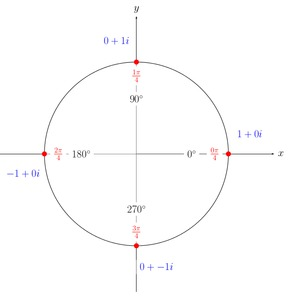
\includegraphics[scale = 0.4]{../images/FourthRoots.jpg}
    \end{center}
    \newcolumn
    \vspace{0.2cm}
    \[
        \begin{split}
            &\lambda^4 - 1 = 0\\
            &\lambda_1 = 1\\
            &\lambda_2 = i\\
            &\lambda_3 = -1\\
            &\lambda_4 = -i
        \end{split}    
    \]
\end{multicols}
We introduce now the complex number $w$ given by:
\[
    w^i = e^{\dfrac{2\pi i}{n}} \overset{\text{in this case}}{\longrightarrow}    w^i = e^{\dfrac{2\pi i}{4}} \implies \begin{cases}
        \lambda_1 = w^0\\
        \lambda_2 = w^1\\
        \lambda_3 = w^2\\
        \lambda_4 = w^3
    \end{cases}
\]
In general we have:
\[
    P_n \implies \lambda^n - 1 = 0 \implies w^0, w^1, \dots, w^{n-1}
\]
Another property of $P$: it's orthogonal indeed $P^\intercal P = I$.
What about the eigenvectors of $P$? Consider the generic matrix $C$ written in terms of $P$:
\[
    C = c_0 I + c_1 P + c_2 P^2 + c_3 P^3    
\]
We want to find the eigenvectors of $C$. If $\lambda_k, \underline{v}_k$ is the couple of eigenvalue and eigenvector of $P$, then:
\[
    \begin{split}
        P\underline{v}_k &= \lambda_k \underline{v}_k\\
        (c_0 I + c_1 P + c_2 P^2 + c_3 P^3)\underline{v}_k &= (c_0 + c_1 \lambda_k + c_2 \lambda_k^2 + c_3 \lambda_k^3)\underline{v}_k\\
    \end{split}
\]
$\underline{v}_k$ is an eigenvector of $C$.\\




\section{Discrete Fourier Transform}

Consider the general theory of eigenvalues and eigenvectors. Given a square matrix \( A \), an eigenvalue \( \lambda \) and an associated eigenvector \( \underline{v} \) are defined such that:
\[
A \underline{v} = \lambda \underline{v}
\]
This implies that the action of the matrix \( A \) on the vector \( \underline{v} \) is equivalent to scaling \( \underline{v} \) by \( \lambda \).

\subsection*{Eigenvalues and Eigenvectors of a Circulant Matrix}
A circulant matrix \( C \) can be defined in terms of its generating vector \( \underline{c} \). The eigenvalues and eigenvectors of \( C \) can be obtained through the Discrete Fourier Transform (DFT). Specifically, if \( \mathbf{F} \) represents the Fourier matrix, then:
\[
C = \mathbf{F}^{-1} \Lambda \mathbf{F}
\]
where \( \Lambda \) is a diagonal matrix containing the eigenvalues of \( C \).

\subsection*{Discrete Fourier Transform (DFT)}
The DFT of a vector \( \underline{c} \) is computed by multiplying it by the Fourier matrix \( \mathbf{F} \):
\[
\mathbf{F} = \frac{1}{\sqrt{n}} \begin{bmatrix}
1 & 1 & 1 & \cdots & 1 \\
1 & w & w^2 & \cdots & w^{n-1} \\
1 & w^2 & w^4 & \cdots & w^{2(n-1)} \\
\vdots & \vdots & \vdots & \ddots & \vdots \\
1 & w^{n-1} & w^{2(n-1)} & \cdots & w^{(n-1)(n-1)}
\end{bmatrix}
\]
where \( w = e^{2\pi i / n} \) is a primitive \( n \)-th root of unity. The DFT transforms a vector into its frequency domain representation.

\subsection*{Eigenvalues of Circulant Matrices}
For a circulant matrix \( C \) generated by vector \( \underline{c} \), its eigenvalues are given by:
\[
\underline{\lambda}_c = \mathbf{F} \underline{c}
\]
Here, \( \underline{\lambda}_c \) represents the vector of eigenvalues of \( C \).

\subsection*{Convolution and Eigenvalues}
Consider two circulant matrices \( C \) and \( D \) generated by vectors \( \underline{c} \) and \( \underline{d} \) respectively. The product \( CD \) is also a circulant matrix. The eigenvalues of \( CD \) are related to the eigenvalues of \( C \) and \( D \) by element-wise multiplication:
\[
\lambda(CD) = \lambda(C) \circledcirc  \lambda(D) = \mathbf{F} \underline{c} \circledcirc  \mathbf{F} \underline{d}
\]
This property arises from the fact that the Fourier transform diagonalizes circulant matrices.

\subsection*{Convolution Theorem}
The convolution of two vectors \( \underline{c} \) and \( \underline{d} \), denoted \( \underline{c} \circledast \underline{d} \), corresponds to the Hadamard product of their Fourier transforms:
\[
\mathbf{F}(\underline{c} \circledast \underline{d}) = \mathbf{F}\underline{c} \circledcirc \mathbf{F}\underline{d}
\]
This is known as the Convolution Theorem and provides a computationally efficient method for computing convolutions using the Fast Fourier Transform (FFT).
With FFT (Fast Fourier Transform) algorithm the first member can be computed with $ N\log(N) + N^2$, while the second term is easier with $(2N\log(N) + N)$and is this the preferred approach.


\section{Optimization in Neural Networks}

A neural network can be seen as a map:
\[
F_{NN}(x) = y
\]

We can define a cost function:
\[
J = \frac{1}{2N} \sum_{i=1}^{N} (\bar{y}_i - y_i)^2
\]

Inside $F_{NN}$, we have nodes that represent weights $w$ and biases $b$, chosen to minimize $J$:
\[
(w, b) = \argmin J
\]

The objective in machine learning is not only to find $w$ and $b$ to build the function $F_{NN}$ minimizing $J$, but also to create $F_{NN}$ capable of making predictions (train set $\neq$ test set).

In the optimization context, we want to get closer to the minimum $J$ without overfitting (i.e., the model should understand the underlying pattern of the data, not just memorize it).

The gradient method, particularly its variant Stochastic Gradient Descent (SGD), is the most used method in machine learning. It is simple and robust (can be implemented with non-convex functions, though theoretical guarantees are for convex ones).

Let's recall its application to linear systems:
\[
Ax = b
\]
with solution $x^*$, where $A \in \mathbb{R}^{n \times n}$ is a symmetric positive definite matrix.

We define the functional:
\[
J(x) = \frac{1}{2} x^T A x - x^T b
\]

To find the minimum:
\[
\begin{aligned}
\nabla J(x) &= Ax - b = 0 \\
&\Rightarrow Ax^* = b
\end{aligned}
\]

\subsubsection*{Algorithm}
Given an initial guess $x^{(0)}$:

For $k = 0, 1, \ldots$:
\begin{enumerate}
    \item $p^{(k)} = -\nabla J(x^{(k)}) = r^{(k)}$
    \item $x^{(k+1)} = x^{(k)} + \alpha_k p^{(k)}$
\end{enumerate}

where $\alpha_k$ is the step length, chosen to minimize $J(x^{(k)} + \alpha p^{(k)})$.

Stopping criteria: $\|r^{(k)}\| \leq \varepsilon$ or $\|x^{(k+1)} - x^{(k)}\| < \varepsilon$

\subsubsection*{Step Length Calculation}
Suppose $x^{(k)}$ and $p^{(k)}$ are given:
\[
\begin{aligned}
J(x^{(k)} + \alpha p^{(k)}) &= \frac{1}{2}(x^{(k)} + \alpha p^{(k)})^T A (x^{(k)} + \alpha p^{(k)}) - (x^{(k)} + \alpha p^{(k)})^T b \\
&= \frac{1}{2}\alpha^2 (p^{(k)})^T A p^{(k)} + \alpha (p^{(k)})^T A x^{(k)} - \alpha (p^{(k)})^T b + \text{constants}
\end{aligned}
\]

Setting the derivative to zero:
\[
\begin{aligned}
\nabla J = 0 &= (p^{(k)})^T A x^{(k)} + \alpha (p^{(k)})^T A p^{(k)} - (p^{(k)})^T b \\
\Rightarrow \alpha &= \frac{(p^{(k)})^T (b -A x^{(k)} )}{(p^{(k)})^T A p^{(k)}} = \frac{(p^{(k)})^T r^{(k)}}{(p^{(k)})^T A p^{(k)}}
\end{aligned}
\]

Define the error, in the energy norm of the matrix A:
\[
e = \frac{1}{2}(x - x^*)^T A (x - x^*)
\]

Error bound:
\[
e(x^{(k)}) \leq \left(\frac{\lambda_{\max} - \lambda_{\min}}{\lambda_{\max} + \lambda_{\min}}\right)^{2k} e(x^{(0)})
\]

where $\lambda_{\max}$ and $\lambda_{\min}$ are the maximum and minimum eigenvalues of $A$.

\subsection*{General Convex Optimization}
Now let $J: \mathbb{R}^d \to \mathbb{R}$ be convex and differentiable, with a global minimum $x^*$. The aim is to find an approximation $\tilde{x}$ of $x^*$ such that:
\[
J(\tilde{x}) - J(x^*) < \varepsilon
\]

\subsubsection*{Algorithm}
Generate a sequence $x^{(0)}, x^{(1)}, \ldots$ using the rule:
\[
x^{(k+1)} = x^{(k)} + v^{(k)}
\]

To guarantee $J(x^{(k+1)}) < J(x^{(k)})$:
\[
\begin{aligned}
J(\mathbf{x}^{(k)} + \mathbf{v}^{(k)}) \approx J(\mathbf{x}^{(k)}) + \nabla J(\mathbf{x}^{(k)})^T\mathbf{v}^{(k)} + \mathcal{O}(\|\mathbf{v}^{(k)}\|^2)
\end{aligned}
\]

Therefore, we can move in the direction of maximum descent by following this rule:

\[
\begin{aligned}
v^{(k)} = -\alpha\nabla J(x^{(k)}), \quad \alpha > 0 \\
x^{(k+1)} = x^{(k)} - \gamma \nabla J(x^{(k)})\\
\end{aligned}
\]

where $\gamma$ is the learning rate.


Remember that:
\begin{itemize}
    \item $\gamma$ can be fixed or can depend on $k$
    \item Choice of $\gamma$ is crucial:
    \begin{itemize}
        \item If too small: very slow procedure
        \item If too large: overshooting (oscillating behavior)
    \end{itemize}
\end{itemize}

\subsection*{Convexity Criterion}
For $J(x), x \in \mathbb{R}^d$, if the domain of $J$ is convex, then $J$ is convex if and only if:
\[
J(y) \geq J(x) + \nabla J(x)^T(y-x) \quad \forall x, y \in \text{dom}(J)
\]
This means the graph of function $J$ lies above the tangent hyperplane to $J$ in $x$.

A convex function has the property of monotonicity of the gradient.\\ \\
\textbf{Monotonicity of the Gradient} \\
A function's gradient \( \nabla f \) is said to be monotone if for all \( x, y \in \mathbb{R}^n \),
\[
(\nabla f(y) - \nabla f(x))^\top (y - x) \geq 0
\]

\subsection{Convergence Analysis}
Let's analyze the convergence of the method. If $J$ is convex, then:
\[
J(x^{(k)}) - J(x^*) \leq \underbrace{\nabla J(x^{(k)})^T}_{e^{(k)}}(x^{(k)} - x^*)
\]

For the iteration that defines the method:
\[
\begin{aligned}
e^{(k)} &= \frac{x^{(k)} - x^{(k+1)}}{\gamma} \\
\Rightarrow (e^{(k)})^T(x^{(k)} - x^*) &= \frac{1}{\gamma}(x^{(k)} - x^{(k+1)})^T(x^{(k)} - x^*)
\end{aligned}
\]

Now I will derive an easy identity:
\begin{enumerate}
\item \(\|v - w\|^2 = (v - w)^T (v - w)\)\\
\item \(\|v - w\|^2 = v^T v - 2v^T w + w^T w\)\\
\item \(\|v - w\|^2 = \|v\|^2 - 2v^T w + \|w\|^2\)\\
\item \(2v^T w = \|v\|^2 + \|w\|^2 - \|v - w\|^2\)\\
\end{enumerate}
Using the identity $2v^Tw = \|v\|^2 + \|w\|^2 - \|v-w\|^2$, we get:
\[
\begin{aligned}
(e^{(k)})^T(x^{(k)} - x^*) &= \frac{1}{2\gamma}[\|x^{(k)} - x^{(k+1)}\|^2 + \|x^{(k)} - x^*\|^2 - \|x^{(k+1)} - x^*\|^2] \\
&= \frac{1}{2\gamma}[\gamma^2\|e^{(k)}\|^2 + \|x^{(k)} - x^*\|^2 - \|x^{(k+1)} - x^*\|^2] \\
&= \frac{\gamma}{2}\|e^{(k)}\|^2 + \frac{1}{2\gamma}[\|x^{(k)} - x^*\|^2 - \frac{1}{2}\|x^{(k+1)} - x^*\|^2]
\end{aligned}
\]

Summing over iterations:
\[
\begin{aligned}
\sum_{k=0}^{T-1}(e^{(k)})^T(x^{(k)} - x^*) &= \frac{\gamma}{2}\sum_{k=0}^{T-1}\|e^{(k)}\|^2 + \frac{1}{2\gamma}[\|x^{(0)} - x^*\|^2 -\frac{1}{2\gamma} \|x^{(T)} - x^*\|^2] \\
&\leq \frac{\gamma}{2}\sum_{k=0}^{T-1}\|e^{(k)}\|^2 + \frac{1}{2\gamma}\|x^{(0)} - x^*\|^2
\end{aligned}
\]

Therefore:
\[
\sum_{k=0}^{T-1}(J(x^{(k)}) - J(x^*)) \leq \frac{\gamma}{2}\sum_{k=0}^{T-1}\|e^{(k)}\|^2 + \frac{1}{2\gamma}\|x^{(0)} - x^*\|^2
\]

\subsection{Convergence Theorem for Lipschitz Convex Functions}
Let $J: \mathbb{R}^d \to \mathbb{R}$ be convex and differentiable, and also:
\begin{itemize}
    \item $\|x^{(0)} - x^*\| \leq R$
    \item $\|\nabla J(x)\| \leq B \quad \forall x$
\end{itemize}

\begin{theorem}
If we choose $\gamma := \frac{R}{B\sqrt{T}}$, then:
\[
\frac{1}{T}\sum_{k=0}^{T-1}(J(x^{(k)}) - J(x^*)) \leq \frac{RB}{\sqrt{T}}
\]
\end{theorem}

To achieve a certain tolerance $\varepsilon$:
\[
\begin{aligned}
\frac{RB}{\sqrt{T}} &< \varepsilon \\
T &\geq \frac{R^2B^2}{\varepsilon^2}
\end{aligned}
\]

Note: There's no dependence on $d$! The number of iterations is $O(1/\varepsilon^2)$.

The previous relation can be bounded:
\[
\sum_{k=0}^{T-1}(J(x^{(k)}) - J(x^*)) \leq \underbrace{\frac{\gamma}{2}B^2T + \frac{R^2}{2\gamma}}_{q(\gamma)}
\]

We want to find $\gamma$ to minimize $q$. Set $q'(\gamma) = 0$:
\[
\begin{aligned}
\frac{1}{2}B^2T - \frac{R^2}{2\gamma^2} &= 0 \\
\gamma &= \frac{R}{B\sqrt{T}}
\end{aligned}
\]

\subsection*{Proof of Convergence Theorem}
\begin{proof}
The previous relation can be bounded:
\[
\sum_{k=0}^{T-1}(J(x^{(k)}) - J(x^*)) \leq \underbrace{\frac{\gamma}{2}B^2T + \frac{R^2}{2\gamma}}_{q(\gamma)}
\]

We want to find $\gamma$ to minimize $q$. Set $q'(\gamma) = 0$:
\[
\begin{aligned}
\frac{1}{2}B^2T - \frac{R^2}{2\gamma^2} &= 0 \\
\gamma &= \frac{R}{B\sqrt{T}}
\end{aligned}
\]

Therefore:
\[
q\left(\gamma = \frac{R}{B\sqrt{T}}\right) = RB\sqrt{T}
\]
\end{proof}

\subsection*{Equivalence of Smoothness and Convexity}


Let $\text{dom}(J)$ be open and convex, and $J: \text{dom}(J) \to \mathbb{R}$ be differentiable. Let $L \in \mathbb{R}^+$. \\ 
$J$ is said to be L-smooth (or smooth with parameter L) if it satisfies the following smoothness inequality for all $x, y \in \text{dom}(J)$:
$$J(y) \leq J(x) + \nabla J(x)^T(y-x) + \frac{L}{2}\|y-x\|^2$$

\begin{lemma}
Let $\text{dom}(J)$ be open and convex, and $J: \text{dom}(J) \to \mathbb{R}$ be differentiable.
Let $L \in \mathbb{R}^+$. The following statements are equivalent:
\begin{enumerate}
    \item $J$ is smooth with parameter $L$
    \item The function $h(x) = \frac{L}{2}x^Tx - J(x)$ is convex over $\text{dom}(h) := \text{dom}(J)$
\end{enumerate}
\end{lemma}


\paragraph{Example 1: $L = 0$}
When $L = 0$, smoothness implies:
\[
J(y) = J(x) + \nabla J(x)^T(y-x)
\]

\paragraph{Example 2: $J(x) = x^2$}
This function is not globally Lipschitz continuous, but it is smooth (has a Lipschitz continuous gradient).

Let's expand $J(y)$ around $x$:
\begin{align*}
J(y) &= y^2 \\
&= (x + (y-x))^2 \\
&= x^2 + 2x(y-x) + (y-x)^2 \\
&= J(x) + \nabla J(x)^T(y-x) + (y-x)^2
\end{align*}

Explanation of the expansion:
\begin{itemize}
    \item $J(x) = x^2$ is our original function at point $x$
    \item $\nabla J(x) = 2x$, so $\nabla J(x)^T(y-x) = 2x(y-x)$
    \item The term $(y-x)^2$ is the remainder
\end{itemize}

This expansion matches the form of the smoothness condition:
\[
J(y) \leq J(x) + \nabla J(x)^T(y-x) + \frac{L}{2}(y-x)^2
\]

In this case, the inequality is an equality with $\frac{L}{2} = 1$, so $L = 2$.

To verify smoothness, we check the gradient condition:
\[
|\nabla J(y) - \nabla J(x)| = |2y - 2x| = 2|y-x| \leq L|y-x|
\]
which is satisfied with $L = 2$.

Therefore, $J(x) = x^2$ is a smooth function with parameter $L = 2$. 
This example illustrates that a function can be smooth without being globally Lipschitz continuous.
\paragraph{Example 3: Quadratic Function}
Consider $J(x) = x^TQx + b^Tx + c$, where:
\begin{itemize}
    \item $Q \in \mathbb{R}^{d \times d}$ is symmetric
    \item $b \in \mathbb{R}^d$
    \item $c \in \mathbb{R}$
\end{itemize}
This function is smooth with $L = 2\|Q\|_2$, where $\|Q\|_2$ is the spectral norm of $Q$.

\textbf{Note:} Subquadratic functions are not necessarily smooth.\subsection*{Equivalence Lemma for Smooth Functions}
\begin{lemma}
Let $J: \mathbb{R}^d \to \mathbb{R}$ be convex and differentiable.
The following statements are equivalent:
\begin{itemize}
    \item $J$ is smooth with parameter $L$
    \item $\|\nabla J(x) - \nabla J(y)\| \leq L\|y-x\| \quad \forall x, y \in \mathbb{R}^d$ (Lipschitz continuity of gradient)
\end{itemize}
\end{lemma}

\subsection{Decreasing Condition Lemma}
\begin{lemma}[Decreasing Condition]
Let $J: \mathbb{R}^d \to \mathbb{R}$ be differentiable and smooth with parameter $L$. With $\gamma := \frac{1}{L}$, the Gradient Descent satisfies:
\[
J(x^{(k+1)}) \leq J(x^{(k)}) - \frac{1}{2L}\|\nabla J(x^{(k)})\|^2 \quad k \geq 0
\]
\end{lemma}

\begin{proof}
The Gradient Descent update is given by:
\[
x^{(k+1)} = x^{(k)} - \frac{1}{L}\nabla J(x^{(k)})
\]

By the smoothness property:
\begin{align*}
J(x^{(k+1)}) &\leq J(x^{(k)}) + (\nabla J(x^{(k)}))^T(x^{(k+1)} - x^{(k)}) + \frac{L}{2}\|x^{(k+1)} - x^{(k)}\|^2 \\
&= J(x^{(k)}) - (\nabla J(x^{(k)}))^T\frac{1}{L}\nabla J(x^{(k)}) + \frac{L}{2}\|\frac{1}{L}\nabla J(x^{(k)})\|^2 \\
&= J(x^{(k)}) - \frac{1}{2L}\|\nabla J(x^{(k)})\|^2
\end{align*}
\end{proof}

\subsection{Convergence Theorem for Smooth Functions}
\begin{theorem}
Let $J: \mathbb{R}^d \to \mathbb{R}$ be differentiable and smooth with parameter $L$.
Choosing $\gamma := \frac{1}{L}$, then for Gradient Descent you have:
\[
J(x^{(T)}) - J(x^*) \leq \frac{L}{2T}\|x^{(0)} - x^*\|^2, \quad \quad  T > 0
\]
where $x^*$ is the optimal point.
\end{theorem}
\\ \\
\begin{proof}
From the decreasing condition lemma, and the usual telescopic sum formula:
\[
\frac{1}{2L}\sum_{k=0}^{T-1}\|\nabla J(x^{(k)})\|^2 \leq \sum_{k=0}^{T-1}(J(x^{(k)}) - J(x^{(k+1)})) = J(x^{(0)}) - J(x^{(T)})
\]
Remembering that:
$$
|| e^{k} ||^2 = || \nabla J(x^{(k)}) ||^2
$$
We know that:
\[
\sum_{k=0}^{T-1}(J(x^{(k)}) - J(x^*)) \leq \frac{\gamma}{2}\sum_{k=0}^{T-1}\|e^{(k)}\|^2 + \frac{1}{2\gamma}\|x^{(0)} - x^*\|^2
\]

For $\gamma = \frac{1}{L}$:
\begin{align*}
\sum_{k=0}^{T-1}(J(x^{(k)}) - J(x^*)) &\leq \frac{1}{2L}\sum_{k=0}^{T-1}\|e^{(k)}\|^2 + \frac{L}{2}\|x^{(0)} - x^*\|^2 \\
&\leq J(x^{(0)}) - J(x^{(T)}) + \frac{L}{2}\|x^{(0)} - x^*\|^2 \\
\Rightarrow \sum_{k=1}^{T}(J(x^{(k)}) - J(x^*)) &\leq \frac{L}{2}\|x^{(0)} - x^*\|^2
\end{align*}

By the decreasing condition lemma, $J(x^{(k+1)}) \leq J(x^{(k)}) \quad \forall \ 0 \leq k \leq T$, so:
\[
J(x^{(T)}) - J(x^*) \leq \frac{1}{T}\sum_{k=1}^{T}(J(x^{(k)}) - J(x^*)) \leq \frac{L}{2T}\|x^{(0)} - x^*\|^2
\]
\end{proof}


\subsection*{Convergence results for Gradient Descent}
\begin{itemize}
    \item Lipschitz-convex functions: $O\left(\dfrac{1}{\epsilon^2}\right)$
    \item Smooth functions: $O\left(\dfrac{1}{\epsilon}\right)$
    \item Smooth and strongy convex functions: $O\left(\dfrac{1}{\log(\epsilon)}\right)$
    \item Accelerated gradient descent: $O\left(\dfrac{1}{\sqrt{\epsilon}}\right)$
\end{itemize}


\section{Accelerated Gradient Descent}
Aim: minimizing convex function $f: \mathbb{R}^d \to \mathbb{R}$ (with gradient $\nabla f$). "First order method" because it only uses the function and its gradient. What is the best first order method?\\
Nemirovski and Yudin (1979): every first order method needs in the worst case $O\left(\dfrac{1}{\sqrt{\epsilon}}\right)$ steps. \\
Nesterov (1983): accelerated gradient descent (AGD). Let $f: \mathbb{R}^d \to \mathbb{R}$ convex, differentiable and smooth with parameter $L$. ADG reads:
\begin{itemize}
    \item choose $\underline{z}^{(0)} = \underline{y}^{(0)} = \underline{x}^{(0)}$
    \item for $k \geq 0$ set:
    \begin{itemize}
        \item $\underline{y}^{(k+1)} = \underline{x}^{(k)} - \dfrac{1}{L} \nabla f(\underline{x}^{(k)})$ \hspace{2cm} Normal step
        \item $\underline{z}^{(k+1)} = \underline{z}^{(k)} - \dfrac{k+1}{2L} \nabla f (\underline{x}^{(k)})$ \hspace{2cm} Aggressive step
        \item $\underline{x}^{(k+1)} = \dfrac{k+1}{k+3} \underline{y}^{(k+1)} + \dfrac{2}{k+3} \underline{z}^{(k+1)}$ \hspace{2cm} Average 
    \end{itemize}
\end{itemize}

\textbf{Theorem of convergence of AGD}: lef $f: \mathbb{R}^d \to \mathbb{R}$ convex, differentiable with a global minimum $\underline{x}^*$ and smooth with parameter $L$. AGD yields:
\[
f(\underline{y}^{(N)}) - f(\underline{x}^*) \leq \dfrac{2L \Vert \underline{z}^{(0)} - \underline{x}^* \Vert^2}{N(N+1)}  \hspace{1cm} N > 0   
\]
\textbf{Definition of smooth and strongly convex functions}: Let $f: \text{dom}(f) \to \mathbb{R}$ be a convex and differentiable function, $X \subseteq \text{dom}(f)$ convex and $\mu \in \mathbb{R}^+$. Function $f$ is called strongly convex with parameter $\mu$ over $X$ if:
\[
f(\underline{y}) \geq f(\underline{x}) + \nabla f(\underline{x})^T (\underline{y} - \underline{x}) + \dfrac{\mu}{2} \Vert \underline{y} - \underline{x} \Vert^2 \hspace{1cm} \forall \underline{x}, \underline{y} \in X    
\] 
Remark
\begin{itemize}
    \item \textbf{smoothness}: $\forall \underline{x} \in X$ the graph of $f$ is below a not-too-steep tangent paraboloid.
    \item \textbf{Strongly-convex}: $\forall \underline{x} \in X$ the graph of $f$ is above a not-too-flat tangent paraboloid.\\ 
\end{itemize}

Theorem of convergence: strongly convex case: let $f: \mathbb{R}^d \to \mathbb{R}$ be a convex, differentiable. Suppose that $f$ is smooth with parameter $L$ and strongly convex with parameter $\mu$ > 0. Choosing:
\[
    \nu = \dfrac{1}{L}    
\]
Gradient Descent with arbitrary initial point $\underline{x}^{(0)}$ satisfies:
\begin{enumerate}
    \item Squared distances to $\underline{x}^*$ are geometrically decreasing: $\Vert \underline{x}^{(k+1)} - \underline{x}^* \Vert^2 \leq \left(1-\dfrac{\mu}{L}\right)\Vert \underline{x}^{(k)} - \underline{x}^* \Vert^2$ \hspace{1cm} $k \geq 0$
    \item Absolute error after N iterations is exponentially small in N: $f(\underline{x}^{(N)}) - f(\underline{x}^*) \leq \dfrac{L}{2}\left(1-\dfrac{\mu}{L}\right)^N \Vert \underline{x}^{(0)} - \underline{x}^* \Vert^2$ \hspace{1cm} $N > 0$
\end{enumerate}
Remember: recalling that $\ln(1+x)\leq x$ we have:
\[
    N \geq \dfrac{L}{\mu} \ln\left(\dfrac{R^2 L}{2\epsilon}\right)    
\]

\subsection*{Derivation of last inequality}

Let $R^2 = \|x^{(0)} - x^*\|^2$. Then:

\[
\frac{LR^2}{2}\left(1 - \frac{\mu}{L}\right)^N \leq \varepsilon
\]

Taking logarithms of both sides:

\[
\ln\left(\frac{LR^2}{2}\right) + N\ln\left(1 - \frac{\mu}{L}\right) \leq \ln(\varepsilon)
\]

Rearranging:

\[
N\ln\left(1 - \frac{\mu}{L}\right) \leq \ln(\varepsilon) - \ln\left(\frac{LR^2}{2}\right)
\]

Dividing both sides by $\ln\left(1 - \frac{\mu}{L}\right)\ln\left(1 - \frac{\mu}{L}\right)$ (note that this is negative, so the inequality flips):

\[
N \geq \frac{\ln\left(\frac{2\varepsilon}{LR^2}\right)}{\ln\left(\frac{L-\mu}{L}\right)}
\]

Now, we can use the inequality $\ln(1+x) \leq x\ln(1+x) \leq x for x > -1x > -1. Let x = -\frac{\mu}{L}x = -\frac{\mu}{L}.$ Then:

\[
\ln\left(1 - \frac{\mu}{L}\right) \leq -\frac{\mu}{L}
\]

Therefore:

\[
N \geq \frac{\ln\left(\frac{2\varepsilon}{LR^2}\right)}{-\frac{\mu}{L}} = \frac{L}{\mu}\ln\left(\frac{LR^2}{2\varepsilon}\right)
\]



\newpage
\section{Stochastic Gradient Descent (SGD)}

In machine learning, cost functions are often written as a finite sum:
\[
J(x) = \frac{1}{N}\sum_{i=1}^N J_i(x)
\]
Since in application we have to compute the gradient of $N$ cost functions to calculate $\nabla J$, the idea is to pick randomly an integer $i(K) \in\{1,2, \ldots, N\}$ at each iteration $K$ and use the following iteration rule.
The SGD update rule is:
\[
x^{(k+1)} = x^{(k)} - \gamma_k \nabla J_{i(k)}(x^{(k)})
\]
where $i(k)$ is randomly chosen from $\{1, 2, \ldots, N\}$ at each iteration.

While in Gradient Descent (GD) the cost function decreases at each iteration, the stochastic version is not monotone (but still converges). It typically consists of two phases:
\begin{enumerate}
    \item It converges quickly to a neighborhood of the solution
    \item It bounces around this neighborhood
\end{enumerate}

\subsection*{Example Cost Function}

Consider the cost function:

\[J(x) = \frac{1}{2} \sum_{i=1}^{N} (a_i x - b_i)^2 \quad a_i, b_i \in \mathbb{R}\]

The gradient and optimal solution are:

\begin{align*}
    \nabla J(x) &= \sum_{i=1}^{N} a_i(a_i x - b_i) = 0 \\
    x^* &= \frac{\sum_{i=1}^{N} a_i b_i}{\sum_{i=1}^{N} a_i^2}
\end{align*}

For individual terms:

\begin{align*}
    \bar{J}_i(x) &= \frac{1}{2}(a_i x - b_i)^2 \quad \text{(parabolas)} \\
    \nabla J_i(x) &= a_i(a_i x - b_i) \\
    x_i^* &= \frac{b_i}{a_i}
\end{align*}

\subsection*{Region of Confusion}

Define the region of confusion as:

\[R := [\min_i x_i^*, \max_i x_i^*] \quad \text{where } x^* \in R\]

The area outside $ \Omega \setminus R$ is called the "far out zone." If $x$ is outside of $R$, then $\nabla J_i(x)$ has the same sign as $\nabla J(x)$.
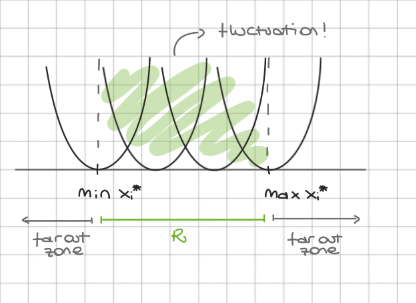
\includegraphics[]{namltexnotes/images/Screenshot 2024-06-26 110851.png}
\\There are two strategies for choosing samples at each iteration:

\begin{enumerate}
    \item Random sampling with replacement
    \item Random sampling without replacement
\end{enumerate}


The second option is better for hardware efficiency, while the first is theoretically better for convergence.

\subsection*{Mini-Batch Approach}

The mini-batch approach uses more than one sample to compute $\nabla J$:

\[\varepsilon_k = \frac{1}{|I_k|} \sum_{i_k \in I_k} \nabla J_{i_k}(x^{(k)}) \quad I_k \subset I\]

where:
\begin{itemize}
    \item If $|I_k| = 1$, we have stochastic gradient descent
    \item If $I_k = I$, we have batch gradient descent
\end{itemize}

This strategy reduces the noise (variance) introduced by using only one sample.
Unlike stochastic gradient descent (SGD) which uses just one sample to compute the gradient, the mini-batch approach uses multiple samples (equal to the batch size) to compute $\nabla J$ (the gradient of the cost function).

The mini-batch gradient estimate is given by:

\begin{equation}
    \varepsilon_{k} = \frac{1}{|I_{k}|} \sum_{i_{k} \in I_{k}} \nabla J_{i_{k}}(x^{(k)})
\end{equation}

Where:
\begin{itemize}
    \item $I_{k}$ is a subset of the full dataset $I$
    \item $|I_{k}|$ is the size of the mini-batch
\end{itemize}

Special cases:
\begin{itemize}
    \item When $|I_{k}| = 1$, you have stochastic gradient descent (SGD)
    \item When $I_{k} = I$ (i.e., the full dataset), you have batch gradient descent
\end{itemize}

Advantages of mini-batch gradient descent:
\begin{itemize}
    \item \textbf{Noise Reduction}: Mini-batch reduces the noise (variance) introduced by using only one sample, as in SGD.
    \item \textbf{Parallelizability}: Mini-batch allows for efficient parallelization of computations, which is particularly beneficial when using GPUs or multi-core CPUs. This leads to faster training times and better hardware utilization.
    \item \textbf{Balance}: It offers a good balance between the frequent updates of SGD and the stability of batch gradient descent.
\end{itemize}

In neural networks, it's generally better not to use very large mini-batches because:
\begin{itemize}
    \item Large mini-batches can create overfitting problems.
    \item They may shrink the region of convergence.
    \item They can potentially reduce the model's generalization ability.
\end{itemize}

The optimal mini-batch size often depends on the specific problem and available computational resources.



\subsection{Equivalent Statements}



The following statements are equivalent:

\begin{enumerate}[a)]
    \item $J(y) \geq J(x) + (\nabla J(x))^T(y-x) + \frac{\mu}{2}\|x-y\|^2$ (strongly convex)
    \item $K(x) = J(x) - \frac{\mu}{2}\|x\|^2$ is convex
    \item $(\nabla J(y) - \nabla J(x))^T(y-x) \geq \mu\|x-y\|^2$
    \item $\frac{1}{2}\|\nabla J(x)\|^2 \geq \mu(J(x) - J(x^*))$ (Polyak-Łojasiewicz (PL) condition)
\end{enumerate}

\subsubsection*{Proof}

\paragraph{(b) $\iff$ (a)}

\begin{align*}
    K(y) & \geq K(x) + \nabla K^\top(x)(y-x) && \text{[given inequality]} \\[10pt]
    \left(J(y) - \frac{\mu}{2}\|y\|^2\right) & \geq \left(J(x) - \frac{\mu}{2}\|x\|^2\right) + \nabla K^\top(x)(y-x) && \text{[substitute $K(y)$ and $K(x)$]} \\[10pt]
    J(y) & \geq J(x) + \frac{\mu}{2}(\|y\|^2 - \|x\|^2) + \left(\nabla J(x) - \mu x^\top\right)(y-x) && \text{[rearrange terms]} \\[10pt]
    & = J(x) + \frac{\mu}{2}(\|y\|^2 - \|x\|^2) + \nabla J^\top(x)(y-x) - \mu x^\top(y-x) && \text{[expand $\nabla K^\top(x)$]} \\[10pt]
    & = J(x) + \nabla J^\top(x)(y-x) + \frac{\mu}{2}(\|y\|^2 - \|x\|^2) - \mu x^\top(y-x) && \text{[group gradient terms]} \\[10pt]
    & = J(x) + \nabla J^\top(x)(y-x) + \frac{\mu}{2}(2x^\top(y-x) + \|y-x\|^2) - \mu x^\top(y-x) && \text{[vector identity]} \\[10pt]
    & = J(x) + \nabla J^\top(x)(y-x) + \mu x^\top(y-x) + \frac{\mu}{2}\|y-x\|^2 - \mu x^\top(y-x) && \text{[distribute $\frac{\mu}{2}$]} \\[10pt]
    & = J(x) + \nabla J^\top(x)(y-x) + \frac{\mu}{2}\|y-x\|^2 && \text{[simplify, cancel terms]}
\end{align*}



\paragraph{(b) ⟹\implies (c)}

By the monotonicity of the gradient:
\begin{align*}
    (\nabla K(y) - \nabla K(x))^\top(y-x) &\geq 0 \quad \forall x, y \\
    \left[\nabla\left(J(y) - \frac{\mu}{2}\|y\|^2\right) - \nabla\left(J(x) - \frac{\mu}{2}\|x\|^2\right)\right]^\top(y-x) &\geq 0 \\
    \left(\nabla J(y) - \nabla J(x) - \mu y + \mu x\right)^\top(y-x) &\geq 0 \\
    (\nabla J(y) - \nabla J(x))^\top(y-x) &\geq \mu(y-x)^\top(y-x) = \mu\|y-x\|^2
\end{align*}

For $x = x^*$:
\[ \nabla J^\top(y)(y-x^*) \geq \mu\|y-x^*\|^2 \]

\paragraph{(a) $\implies$ (d)}

Minimize each term of (a):
\begin{itemize}
    \item LHS: $J(x^*)$
    \item RHS: $\nabla J(x) + \mu(y-x) = 0$
\end{itemize}
Therefore:
\begin{align*}
    y &= x - \frac{1}{\mu}\nabla J(x) \\
 J(x^*) & \geq J(x) - \frac{1}{\mu}\nabla J^T(x)\nabla J(x) + \frac{1}{2\mu}\|\nabla J(x)\|^2 \\
   J(x^*)  &\geq J(x) - \frac{1}{2\mu}\|\nabla J(x)\|^2
\end{align*}
Which is equivalent to:
\begin{equation*}
    \frac{1}{2}\|\nabla J(x)\|^2 \geq \mu(J(x) - J(x^*))
\end{equation*}
This completes the proof of (a) $\implies$ (d).

Let's continue the discussion on stochastic gradient descent method. We recall the cost function:
\[
    J(\underline{w}) = \dfrac{1}{N}\sum_{i=1}^N J_i(\underline{w})    
\]
And the algorithm is the following:
\begin{itemize}
    \item Sample $i_k$ randomly from $\{1, \dots, N\}$.
    \item Update $\underline{w}_{k+1} = \underline{w}_k - \gamma_k \underbrace{\nabla J_{i_k}(\underline{w}_k)}_{g_k = \text{stochastic gradient}}$.
\end{itemize}

\subsection{Simple convergence results for SGD}
Consider two quantities:
\begin{itemize}
    \item $J(\underline{w}^{(k+1)}) - J(\underline{w}^*)$
    \item $\mathbb{E}[J(\underline{w}^{(k+1)}) - J(\underline{w}^*)]$
\end{itemize}
These are two measures to evaluate the convergence of the algorithm. We can consider convergence in expectation.
We have two main results:
\text{Assume:}

\begin{enumerate}
    \item $J$ is smooth (L-Lipschitz):
    \[J(y) \leq J(x) + (\nabla J(x))^T(y-x) + \frac{L}{2}\|x-y\|^2\]
    
    \item $J$ is strongly convex:
    \[J(y) \geq J(x) + (\nabla J(x))^T(y-x) + \frac{\mu}{2}\|x-y\|^2\]
    
    \item $\|\nabla J_t(x)\| \leq c$ for some $c > 0$
    
    \item $0 < 2 \mu \gamma \leq 1$ for some constant $\gamma$
    
    \item $\mathbb{E}[\nabla J_t(x)] = \nabla J(x)$ (unbiased estimator)
\end{enumerate}
Then we have that:
\begin{enumerate}
    \item $\mathbb{E}[J(\underline{w}^{(k)}) - J(\underline{w}^*)] \leq (1-2\mu \gamma)^k [J(\underline{w}^{(0)}) - J(\underline{w}^*)] + \dfrac{L\gamma C^2}{4\mu}$
    \item $\mathbb{E}[\|x^*-z^k\|^2] \leq (1-2\gamma\mu)^k (J(x^0) - J(x^*)) + \frac{\gamma C^2}{2 \mu}$
\end{enumerate}

The linear convergence is polluted by a factor bounded by $\gamma$.


\subsection*{Proof}

Assuming $J$ is smooth:


   By smoothness of $J$:
    \begin{equation*}
        J(x^{k+1}) \leq J(x^k) + (\nabla J(x^k))^\top(x^{k+1} - x^k) + \frac{L}{2}\|x^{k+1} - x^k\|^2
    \end{equation*}

  Substituting $x^{k+1} = x^k - \gamma \nabla J_{ik}(x^k)$:
    \begin{equation*}
        J(x^{k+1}) \leq J(x^k) + \nabla J(x^k)^\top(-\gamma \nabla J_{ik}(x^k)) + \frac{L\gamma^2}{2}\|\nabla J_{ik}(x^k)\|^2
    \end{equation*}

Using the bound $\|\nabla J_{ik}(x^k)\|^2 \leq C^2$:
    \begin{equation*}
        J(x^{k+1}) \leq J(x^k) - \gamma \nabla J(x^k)^\top \nabla J_{ik}(x^k) + \frac{L\gamma^2 C^2}{2}
    \end{equation*}

  Taking expectation, and using the fact that $\nabla J_{ik}(x^k)$ is an unbiased estimator of $\nabla J(x^k)$::
    \begin{equation*}
        \mathbb{E}[J(x^{k+1})] \leq \mathbb{E}[J(x^k) - \gamma \nabla J(x^k)^\top \nabla J(x^k)] + \frac{L\gamma^2 C^2}{2}
    \end{equation*}


    \begin{equation*}
        \mathbb{E}[J(x^{k+1})] \leq J(x^k) - \gamma \|\nabla J(x^k)\|^2 + \frac{L\gamma^2 C^2}{2}
    \end{equation*}

   Subtracting $J(x^*)$ from both sides:
    \begin{equation*}
        \mathbb{E}[J(x^{k+1}) - J(x^*)] \leq J(x^k) - J(x^*) - \gamma \|\nabla J(x^k)\|^2 + \frac{L\gamma^2 C^2}{2}
    \end{equation*}

   Using the PL condition for strongly convex functions: $\|\nabla J(x^k)\|^2 \geq 2\mu(J(x^k) - J(x^*))$:
    \begin{equation*}
        \mathbb{E}[J(x^{k+1}) - J(x^*)] \leq (1-2\gamma\mu)(J(x^k) - J(x^*)) + \frac{L\gamma^2 C^2}{2}
    \end{equation*}

    Applying this inequality recursively, and bounding the resulting geometric series:
    \begin{equation*}
        \mathbb{E}[J(x^{k+1}) - J(x^*)] \leq \left(1 - 2 \delta \mu\right)^{k+1} \left(J(x^0) - J(x^*)\right) + \sum_{i=0}^{k+1} \left(1 - 2 \gamma \mu\right)^i \frac{L \gamma^2 C}{2}  \\
\leq (1-2\gamma\mu)^{k+1}(J(x^0) - J(x^*)) + \frac{L\gamma C^2}{4\mu}
    \end{equation*}

This proves the first result. For the second result:\\

     Consider $\|x^{k+1} - x^*\|^2$:
    \begin{equation*}
        \|x^{k+1} - x^*\|^2 = \|x^k - \gamma\nabla J_{ik}(x^k) - x^*\|^2
    \end{equation*}

     Expanding:
    \begin{equation*}
        \|x^{k+1} - x^*\|^2 = \|x^k - x^*\|^2 - 2\gamma\nabla J_{ik}(x^k)^\top(x^k - x^*) + \gamma^2\|\nabla J_{ik}(x^k)\|^2
    \end{equation*}

     Using the bound $\|\nabla J_{ik}(x^k)\|^2 \leq C^2$:
    \begin{equation*}
        \|x^{k+1} - x^*\|^2 \leq \|x^k - x^*\|^2 - 2\gamma\nabla J_{ik}(x^k)^\top(x^k - x^*) + \gamma^2C^2
    \end{equation*}

     Taking expectation:
    \begin{equation*}
        \mathbb{E}[\|x^{k+1} - x^*\|^2] \leq \|x^k - x^*\|^2 - 2\gamma\nabla J(x^k)^\top(x^k - x^*) + \gamma^2C^2
    \end{equation*}

     Using strong monotonicity of the gradient for strongly convex functions, and the fact that at $x*$ the gradient is null: $\nabla J(x^k)^\top(x^k - x^*) \geq \mu\|x^k - x^*\|^2$:
    \begin{equation*}
        \mathbb{E}[\|x^{k+1} - x^*\|^2] \leq (1-2\gamma\mu)\|x^k - x^*\|^2 + \gamma^2C^2
    \end{equation*}

     Applying this inequality recursively, and bounding the resulting geometric series as previously:
    \begin{equation*}
        \mathbb{E}[\|x^{k+1} - x^*\|^2] \leq (1-2\gamma\mu)^{k+1}\|x^0 - x^*\|^2 + \frac{\gamma C^2}{2\mu}
    \end{equation*}

This proves the second result.

\subsection*{Convergence Properties}
SGD with a constant learning rate and single-sample gradient computation exhibits linear convergence. This linear convergence applies to both:

\begin{itemize}
    \item The value of the objective function
    \item The values of the parameter iterates
\end{itemize}

The convergence is affected by a constant factor that depends on the chosen learning rate, as shown previously.:


\subsection*{Importance of Learning Rate ($\gamma$)}
Up to this point, we've considered $\gamma$ as a fixed value. The choice of $\gamma$ is crucial:

\begin{itemize}
    \item If $\gamma$ is too small: The algorithm converges slowly, leading to high computational costs.
    \item If $\gamma$ is too large: The algorithm may fail to converge or even diverge.
\end{itemize}

The learning rate doesn't have to remain constant throughout the optimization process. It can be adjusted in two ways:

\begin{enumerate}[label=(\alph*)]
    \item \textbf{Iteration-based:} The learning rate changes from one iteration to the next.
    \item \textbf{Parameter-specific:} Different parameters within the model can have individualized learning rates.
\end{enumerate}

These adaptive strategies can help balance convergence speed and stability, potentially leading to more efficient optimization. Common adaptive learning rate methods include:

\begin{itemize}
    \item AdaGrad
    \item RMSprop
    \item Adam
\end{itemize}

Each of these methods adjusts the learning rate based on the historical gradient information, allowing for more nuanced optimization trajectories.

\subsubsection*{Line Search Procedure}
Example of picking learning rate varying on the iteration ($\gamma_k$):
\begin{itemize}
    \item initial guess: $\underline{w}^{(0)}$
    \item pick a direction $\underline{P}_k$ such that $\underline{P}_k^\intercal \nabla J(\underline{w}^{(k)}) < 0$ (i.e direction towards the minimum)
    \item typically $\underline{P}_k = \dfrac{-\nabla J(\underline{w}^{(k)})}{\|\nabla J(\underline{w}^{(k)})\|}$
    \item $\underline{w}^{(k+1)} = \underline{w}^{(k)} + \gamma_k\underline{P}_k$
    \item $\gamma_k$ is chosen to minimize ($\arg\min_{\gamma}$) $J(\underline{w}^{(k)} + \gamma_k\underline{P}_k)$
\end{itemize}
Obviously the choice of $\gamma_k$ is a minimization problem, that can be solved by means of analytical methods or by iterative procedures depending on the case. \\
\textbf{Example}\\
Consider the function:
\[J(\underline{x}) = x_1 - x_2 + 2x_1x_2 + 2x_1^2 + x_2^2\]
\[
    \underline{x} = \begin{bmatrix}
        x_1\\x_2
    \end{bmatrix} \hspace{2cm}
    \nabla J(\underline{x}) = \begin{bmatrix}
        1 + 2x_2 + 4x_1\\-1 + 2x_1 + 2x_2
    \end{bmatrix}    
\]
Let's define the initial guess and so the initial gradient:
\[
    \underline{x}^{(0)} = 
    \begin{bmatrix}
        0\\0
    \end{bmatrix} \hspace{2cm}
    \nabla J(\underline{x}^{(0)}) =
    \begin{bmatrix}
        1\\-1
    \end{bmatrix}    
\]
Now, we have to solve:
\[
    J(\underline{x}^{(0)} - \gamma \nabla J(\underline{x}^{(0)})) = J\left(  
        \begin{bmatrix}
            0\\0
        \end{bmatrix}-
        \gamma 
        \begin{bmatrix}
            1\\-1
        \end{bmatrix}
    \right) = J\left(  
        \begin{bmatrix}
            -\gamma\\
            \gamma
        \end{bmatrix}
        \right) = \gamma^2 - 2\gamma
\]
Now we have to minimize this function so we compute the derivative and set it to 0:
\[
    \dfrac{d}{d\gamma} J\left(  
        \begin{bmatrix}
            -\gamma\\
            \gamma
        \end{bmatrix}
        \right) = 2\gamma - 2 = 0 \implies \gamma = 1
\]
This means that, for the first iteration, the value of the learning rate which minimizes the function is $\gamma = 1$. This can be done for each iteration. 
This procedure is like cutting the function in one direction and then choose the learning rate which minimizes that 1D function. 


\subsection*{SDG with Momentum}




Standard Gradient Descent (GD) only considers the current gradient and learning rate at each iteration, without taking into account past steps. This leads to two main problems:

\begin{enumerate}
    \item The gradient of the cost function becomes negligible at plateaus or saddle points, resulting in minimal updates.
    \item The path followed can be highly oscillatory, even with mini-batch techniques.
\end{enumerate}

Momentum addresses these issues by incorporating contributions from previous directions. This allows Gradient Descent with Momentum to take larger steps in directions where past gradients have been consistent, and smaller steps when the gradient oscillates.

The update rule for Gradient Descent with Momentum is given by:

\begin{equation}
    x_{t+1} = x_t - \gamma_t \nabla J_i(x_t) + \beta(x_t - x_{t-1})
\end{equation}

where:
\begin{itemize}
    \item $x_t$ is the parameter vector at iteration $t$
    \item $\gamma_t$ is the learning rate at iteration $t$
    \item $\nabla J_i(x_t)$ is the gradient of the cost function with respect to $x_t$
    \item $\beta$ is the momentum constant
\end{itemize}

The momentum constant $\beta$ typically ranges from 0.8 to 0.99:

\begin{equation}
    \beta \in [0.8, 0.99]
\end{equation}

Both $\gamma$ (learning rate) and $\beta$ (momentum constant) are hyperparameters. They are not automatically tuned or optimized, but must be chosen a priori. Their selection is crucial for achieving good results. Proper tuning of these hyperparameters is fundamental to the success of the Gradient Descent with Momentum algorithm.

To address this problem, \textbf{Adadelta} and \textbf{RSMProp} take some sort of average gradients.



% \include{Lecture17}
% \include{Lecture18}


\newtheorem{theorem}{Theorem}


\section{Newton's Method}

We begin by reviewing Newton's method in one dimension for two contexts: finding the root of a function and finding the minimum of a function. We then extend the method to higher dimensions. Recall that a function $f$ is $C^2$ if $f$ is twice differentiable and $f''$ is continuous.


\subsubsection*{Root-Finding Problem}

Let $\alpha$ be a zero of $f$. For $f \in C^2(\mathbb{R})$:

\begin{equation}
    f(\alpha) = 0 = f(x) + (\alpha - x)f'(\xi)
\end{equation}

where $\xi$ is between $x$ and $\alpha$. This leads to the iterative formula:

\begin{equation}
    x^{(k+1)} = x^{(k)} - \frac{f(x^{(k)})}{f'(x^{(k)})} \quad \forall k \geq 0
\end{equation}

given an initial guess $x^{(0)}$.

\subsubsection*{Minimization Problem}

For $f \in C^2(\mathbb{R})$, we use the second-order Taylor approximation:

\begin{equation}
    f(x^{(k)} + \epsilon) = f(x^{(k)}) + \epsilon f'(x^{(k)}) + \frac{\epsilon^2}{2}f''(x^{(k)}) \tag{$\star$}
\end{equation}

To minimize this approximation, we set its derivative to zero:

\begin{equation}
    \frac{d}{d\epsilon}(\star) = f'(x^{(k)}) + \epsilon f''(x^{(k)}) = 0 \implies \epsilon = -\frac{f'(x^{(k)})}{f''(x^{(k)})}
\end{equation}

This yields the iterative formula:

\begin{equation}
    x^{(k+1)} = x^{(k)} - \frac{f'(x^{(k)})}{f''(x^{(k)})} \quad \forall k \geq 0 \tag{$\star\star$}
\end{equation}

given an initial guess $x^{(0)}$.

\subsubsection*{Multi-Dimensional Newton's Method}

The goal of Newton's method in higher dimensions is to find:

\begin{equation}
    \min_{\underline{w}} J(\underline{w})
\end{equation}

A necessary condition for $\underline{w}^*$ to be a minimum is that $\nabla J(\underline{w}^*) = \underline{0}$. 

The multi-dimensional Newton's method is a generalization of ($\star\star$):

\begin{equation}
    \underline{w}^{(k+1)} = \underline{w}^{(k)} - \mathbf{H} (\underline{w}^{(k)})^{-1}\nabla J(\underline{w}^{(k)}) \quad \forall k \geq 0
\end{equation}

where $\mathbf{H} (\underline{w}^{(k)})$ is the Hessian matrix of $J$ at $\underline{w}^{(k)}$. Note that $\mathbf{H} (\underline{w}^{(k)})$ must be non-singular for this method to work.

We define the search direction:

\begin{equation}
    \underline{d}(\underline{w}^{(k)}) = - \mathbf{H} (\underline{w}^{(k)})^{-1}\nabla J(\underline{w}^{(k)})
\end{equation}

\textbf{Note:} If $J$ is convex, then $\mathbf{H} (\underline{w}^{(k)})$ is positive definite, implying:

\begin{equation}
    \underline{d}(\underline{w}^{(k)})^\top \nabla J(\underline{w}^{(k)}) = - \nabla J(\underline{w}^{(k)})^\top \mathbf{H} (\underline{w}^{(k)})^{-1}\nabla J(\underline{w}^{(k)}) < 0
\end{equation}

This means that $\underline{d}(\underline{w}^{(k)})$ is a descent direction. If $J$ is not convex, Newton's method may converge to local minimizers or saddle points.

\begin{theorem}
Let $J \in C^2(\mathbb{R}^n)$, the Hessian be L-Lipschitz continuous, and $\underline{w}^*$ be a stationary point. If $\mathbf{H} (\underline{w}^*)$ is nonsingular, then there exists a neighborhood of $\underline{w}^*$, denoted $\mathcal{B}_{\rho}(\underline{w}^*)$ (a ball of radius $\rho$ centered at $\underline{w}^*$), such that for any $\underline{w}^{(0)} \in \mathcal{B}_{\rho}(\underline{w}^*)$, the sequence generated by Newton's method converges quadratically to $\underline{w}^*$, and each iteration $\underline{w}^{(k)}$ remains in $\mathcal{B}_{\rho}(\underline{w}^*)$.
\end{theorem}

\textbf{Note:} $\rho$ depends on the Hessian, and $\underline{w}^*$ is typically unknown. $\mathcal{B}_{\rho}(\underline{w}^*)$ is called the domain of quadratic attraction of $\underline{w}^*$.\\

\textbf{Computational Consideration:} Computing the Hessian $\mathbf{H}$ and solving $\mathbf{H}\underline{d} = \nabla J$ is computationally expensive, especially for high-dimensional problems.\\

\subsection{Quasi-Newton method}
The idea is to approximate the Hessian with a matrix $\mathbf{B}_k = \mathbf{H}(\underline{w}^{(k)})$ which is positive definite and invertible. We then set 
\[
    \underline{w}^{(k+1)} = \underline{w}^{(k)} + \alpha_k \underline{d}_k 
\]
Where $\underline{d}_k$ is the direction of descent and $\alpha_k$ is the step size. In particular, we set $\underline{d}_k = - \mathbf{B}_k^{-1}\nabla J(\underline{w}^{(k)})$.\\

The algorithm is the following:
\begin{enumerate}
    \item Choose $\underline{w}^{(0)} \in \mathbb{R}^n$, $\mathbf{B}_0 \in \mathbb{R}^{n \times n}$ nonsingular (often $\mathbf{B}_0 = I$), $\epsilon > 0$ and $k = 0$
    \item If $\|\nabla J(\underline{w}^{(k)})\| < \epsilon$ stop
    \item Compute $\underline{d}_k = - \mathbf{B}_k^{-1}\nabla J(\underline{w}^{(k)})$
    \item Perform a line-search for minimizing $\phi(\alpha) = J(\underline{w}^{(k)} + \alpha\underline{d}_k)$: find $\alpha_k$ that satisfy the Wolfe conditions and set $\underline{w}^{(k+1)} = \underline{w}^{(k)} + \alpha \underline{d}_k$ 
    \item Compute $\mathbf{B}_{k+1}$ (according to some rule)
    \item $k \to k+1$, goto step 2
\end{enumerate}
$\alpha_k$ satisfy the Wolfe conditions if, for a given direction $\underline{d}_k$:
\begin{enumerate}
    \item $J(\underline{w}^{(k)} + \alpha_k\underline{d}_k) \leq J(\underline{w}^{(k)}) + c_1 \alpha_k \underline{d}_k^\intercal \nabla J(\underline{w}^{(k)}) $ (Armijo condition)
    \item $- \underline{d}_k^\intercal \nabla J(\underline{w}^{(k)} + \alpha_k\underline{d}_k) \leq -c_2 \underline{d}_k^\intercal \nabla J(\underline{w}^{(k)})$ (curvature condition)
\end{enumerate}
And $0 < c_1 < c_2 < 1$.\\

\textbf{Remember: } the first condition is a sufficient decrease condition on values of $\alpha_k$, the second condition is a curvature condition (reduction of the slope). They give an upper and lower bound on $\alpha_k$.\\

\textbf{Remember: } if $\underline{d}_k = - \mathbf{B}_k^{-1}\nabla J(\underline{w}^{(k)})$ and $\textbf{B}_k$ is positive definite then if $\textbf{B}_k$ is properly updated then also $\textbf{B}_{k+1}$ is positive definite. \\


Let's now list all the desired properties of $\mathbf{B}_k$:
\begin{enumerate}[i]
    \item $\textbf{B}_k$ should be non-singular
    \item $\textbf{B}_k$ should be such that $\underline{d}_k$ is a descent direction
    \item $\textbf{B}_k$ should be symmetric (as $\textbf{H}$)
    \item $\textbf{B}_{k+1}$ should be computable by using $\nabla J(\underline{w}^{(k+1)}), \nabla J(\underline{w}^{(k)}), \dots, \nabla J(\underline{w}^{(0)}), \underline{d}_k, \alpha_k$.
    \item $\textbf{B}_{k+1}$ should be "close" to $\textbf{B}_{k}$ (so $\textbf{B}_{k}$ can converge to $\textbf{H}(\underline{w}^*)$ and $\underline{d}_k$ is allowed to become the Newton step asymptotically)
    \item $\textbf{B}_{k}$ should be such that the computational cost per iteration is at most $O(n^2)$ compared to $O(n^3)$ for the Newton method. 
\end{enumerate}

\textbf{Remember}: $i$ and $iii$ are satisfied if $\textbf{B}_k$ is symmetric positive definite. For $ii$ we have:
\[
    \underline{d}_k^\intercal \nabla J(\underline{w}^{(k)}) = -\nabla J(\underline{w}^{(k)})^\intercal \mathbf{B}_k^{-1} \nabla J(\underline{w}^{(k)}) < 0 \iff \textbf{B}_k \text{ is positive definite}    
\]
This avoids also QN method to get attracted to any point but a local minimizer.\\

\textbf{Remember: } $iv$ can be obtained if the "secant condition" is satisfied, i.e.:
\[
    \mathbf{B}_{k+1} \underline{\delta}_k = \underline{\gamma}_k   
\]
Where
\[
    \underline{\gamma}_k = \nabla J(\underline{w}^{(k+1)}) - \nabla J(\underline{w}^{(k)}) \hspace{0.2cm} \text{ and } \hspace{0.2cm} \underline{\delta}_k = \alpha_k \underline{d}_k
\]

\textbf{Remember: } to quantify the distance between $\textbf{B}_{k+1}$ and $\textbf{B}_{k}$ we can use a norm or by keeping the rank of $\textbf{B}_{k+1} - \textbf{B}_{k}$ as low as possible.\\

\subsection{Symmetric rank 1 updates}
$iii$ and $iv$ can be satisfied by requiring:
\[
    \mathbf{B}_{k+1} = \mathbf{B}_k + \underline{u}\underline{u}^\intercal \hspace{0.3cm} \text{rank 1 update}   
\]
By enforcing the secant conditions. In particular:
\[
    \mathbf{B}_{k+1} = \mathbf{B}_k + \underline{u}\underline{u}^\intercal \implies \mathbf{B}_{k+1} \underline{\delta}_k = \mathbf{B}_k \underline{\delta}_k + (\underline{u}\underline{u}^\intercal) \underline{\delta}_k \implies (\underline{u}^\intercal \underline{\delta}_k)\underline{u} = \underline{\gamma}_k - \mathbf{B}_k \underline{\delta}_k
\]
Transposing and multiplying by $\underline{\delta}_k$:
\[
    (\underline{u}^\intercal \underline{\delta}_k)^2 = (\underline{\gamma}_k - \mathbf{B}_k\underline{\delta}_k)^\intercal \underline{\delta}_k \implies \underline{u} = \frac{\underline{\gamma}_k - \mathbf{B}_k\underline{\delta}_k}{\underline{u}^\intercal \underline{\delta}_k}    
\]
Hence
\[
    \mathbf{B}_{k+1} = \mathbf{B}_k + \frac{(\underline{\gamma}_k - \mathbf{B}_k\underline{\delta}_k)(\underline{\gamma}_k - \mathbf{B}_k\underline{\delta}_k)^\intercal}{(\underline{\gamma}_k - \mathbf{B}_k\underline{\delta}_k)^\intercal \underline{\delta}_k}    \hspace{0.2cm} \text{SR1}
\]
Since $\underline{\gamma}_k = \nabla J (\underline{w}^{(k+1)}) - \nabla J (\underline{w}^{(k)})$ and $\underline{\delta}_k = \alpha_k \underline{d}_k$ the update requires only already known quantities.\\

SR1 is 
\begin{itemize}
    \item positive: easy to compute
    \item negative: $\mathbf{B}_k$ not always positive
    \item negative: $\underline{d}_k$ might not always be defined or be a descent direction
    \item negative: $(\underline{\gamma}_k - \mathbf{B}_k\underline{\delta}_k)^\intercal\underline{\delta}_k$ can be close to zero so we can have large updates
\end{itemize}

\textbf{Remember: } When $\underline{d}_k$ is known the computations of $\alpha_k, w^{(k+1)},\nabla J(\underline{w}^{(k+1)}), \underline{\gamma}_k$ and $\underline{d}_k$ are very cheap. The computation of the outer product requires computing $n^2$ entries, adding 2 $n\times n$ matrices requires $n^2$ additions so the cost is $O(n^2)$. But we have also to solve the linear system, if $d_k$ is unknown:
\[
    \mathbf{B}_k\underline{d}_k = - \nabla J(\underline{w}^{(k)})\hspace{0.5cm} O(n^3)\text{ ops required}    
\]

\textbf{Theorem (Sherman-Morrison-Woodbury): } if $B \in \mathbb{R}^{n\times n}$ and $U,V \in \mathbb{R}^{n \times p}$ then 
\[
    (B + UV^\intercal)^{-1} = B^{-1} - B^{-1}U(I + V^\intercal B^{-1}U)^{-1}V^\intercal B^{-1}    
\]

\textbf{Remember: } if we knew $A_k = \mathbf{B}_k^{-1}$, applying SMW to $B_{+} = \mathbf{B}_{k+1}, B = \mathbf{B}_k, U = \underline{u} = (\underline{\gamma}_k - \mathbf{B}_k\underline{\delta}_k)$ and $V = U^\intercal \hspace{0.1cm}(p=1)$ we have:
\[
    A_{k+1} = (B_+)^{-1} = B^{-1} - B^{-1}\underline{u}(1+\underline{u}^\intercal B^{-1}\underline{u})^{-1}\underline{u}^\intercal B^{-1} = A_k + \dfrac{(\underline{\delta}_k - A_k\underline{\gamma}_k)(\underline{\delta}_k - A_k\underline{\gamma}_k)^\intercal}{(\underline{\delta}_k - A_k\underline{\gamma}_k)^\intercal \underline{\gamma}_k}
\] 
This implies that $A_{k+1}$ is a rank 1 update of $A_k$. Since we have assumed that $A_k$ is known, computing $\underline{d}_k = -A_k \nabla J(\underline{w}^{(k)})$ is $O(n^2)$. Hence computing $\underline{\delta}_k$ and $\underline{\gamma}_k$ is $O(n^2)$ plus the outer product which is $O(n^2)$. $A_{k+1}$ can be computed from $A_k$ in $O(n^2)$. \\

\textbf{Remember: } if we start with $\mathbf{B}_0$ with known inverse (for example $\mathbf{B}_0 = I$) then we never need to build $\mathbf{B}_k$. \\

\textbf{Remember: } SR1 converges superlinearly in a neighborhood of a local minimizer \footnote[2]{A converging sequence $x^{(k)} \to x^*$ has a convergence rate $r\geq 1$ if $\exists \rho > 0$ and $k_0$ such that 
\[
    \|x^{(k+1)} - x^*\| \leq \rho \|x^{(k)} - x^*\|^r \hspace{0.2cm} \forall k \geq k_0 \hspace{1cm} \lim_{k \to \infty} \frac{\|x^{(k+1)} - x^*\|}{\|x^{(k)} - x^*\|} = 0 \hspace{0.2cm} \text{superlinear convergence}
\]
for $r = 1$ then $\rho < 1.$
}.

\textbf{Drawbacks of SR1:} $\mathbf{B}_k$ is not guaranteed to be positive definite, $\underline{d}_k$ is not guaranteed to be a descent direction.\\


\subsection{BFGS}
The Broyden-Fletcher-Goldfarb-Shanno algorithm satisfies all properties, from $i$ to $vi$. The idea is:
\[
    \mathbf{B}_{k+1} = \mathbf{B}_k + \underline{u}\underline{u}^\intercal + \underline{v}\underline{v}^\intercal \hspace{0.3cm} \underline{u},\underline{v}\text{ linearly independent} 
\] 
So it is a rank 2 update. Important to remember that SR1 was the best rank 1 update while this method, BFGS, is the best rank 2 update.
\[
    \mathbf{B}_{k+1} = \mathbf{B}_k - \frac{\mathbf{B}_k\underline{\gamma}_k\underline{\gamma}_k^\intercal \mathbf{B}_k}{\underline{\delta}_k^\intercal \mathbf{B}_k \underline{\delta}_k} + \frac{\underline{\gamma}_k\underline{\gamma}_k^\intercal}{\underline{\gamma}_k^\intercal \underline{\delta}_k} \hspace{0.3cm} \text{ where } \begin{cases}
        \underline{\gamma}_k = \nabla J(\underline{w}^{(k+1)}) - \nabla J(\underline{w}^{(k)})\\
        \underline{\delta}_k = \underline{w}^{(k+1)} - \underline{w}^{(k)} = \alpha_k \underline{d}_k
    \end{cases}
\]

\textbf{Remember: }\\
When the search direction \(\underline{d}_k\) is known, the computational cost of the BFGS update consists of two main parts:

\begin{itemize}
  \item The update itself: \(O(n^2)\) operations, where \(n\) is the dimension of the optimization problem.
  \item Solving the linear system \(\mathbf{B}_k \underline{d}_k = -\nabla J(\underline{w}^{(k)})\) to find the next search direction. The solution of this linear system can be efficiently computed using the Sherman-Morrison-Woodbury (SMW) formula, which takes advantage of the low-rank structure of the update. 
\end{itemize}


A reduction in complexity is obtained using Cholensky factorization. If $\mathbf{B}_k$ is positive definite and we know $\mathbf{B}_k = \mathbf{L}_k \mathbf{L}_k^\intercal$ where $\mathbf{L}_k$ is lower triangular, then:
\[
    \mathbf{B}_k \underline{d}_k = - \nabla J(\underline{w}^{(k)}) \iff \begin{cases}
        \mathbf{L}_k \underline{g}_k = - \nabla J(\underline{w}^{(k)})\\
        \mathbf{L}_k^\intercal \underline{d}_k = \underline{g}_k
    \end{cases}
\]

If the Cholensky decomposition of $\mathbf{B}_k$ is known then computing $\underline{d}_k$ is $O(n^2)$ and so the cost of BFGS per iteration is $O(n^2)$ as well.\\

\textbf{Idea: } 
\begin{itemize}
    \item find an update rule $L_k \leftarrow L_{k+1}$ (minimizing $d(L_{k+1}, L_k)$)
    \item compute $\mathbf{B}_{k+1} = \mathbf{L}_{k+1}\mathbf{L}_{k+1}^\intercal$ (positive definite)
    \item $L_{k+1}$ is chosen such that $\mathbf{B}_{k+1}$ satisfies the secant conditions (property $iv$)
\end{itemize}

\textbf{The actual BFGS algorithm:}
\begin{enumerate}
    \item Choose $\underline{w}^{(0)}$ and $L_0$ with positive diagonal entries ($L_0 = I$); choose $\epsilon > 0$
    \item If $\|\nabla J(\underline{w}^{(k)})\| < \epsilon$ stop
    \item Otherwise solve $\mathbf{L}_k \underline{g}_k = - \nabla J(\underline{w}^{(k)})$ and $\mathbf{L}_k^\intercal \underline{d}_k = \underline{g}_k$
    \item Perform a line search to find $\alpha_k > 0$ such that $J(\underline{w}^{(k)} +  \alpha\underline{d}_k) < J(\underline{w}^{(k)})$ and such that the Wolfe conditions are satisfied
    \item Set $\underline{\delta}_k = \alpha_k \underline{d}_k$, $\underline{w}^{(k+1)} = \underline{w}^{(k)} + \underline{\delta}_k$. Compute $\underline{\gamma}_k = \nabla J(\underline{w}^{(k+1)}) - \nabla J(\underline{w}^{(k)})$ and $\beta_k = \pm \sqrt{\dfrac{\underline{\gamma}_k^\intercal\underline{\delta}_k}{\underline{\delta}_k^\intercal \mathbf{B}_k \underline{\delta}_k}}$
    \item Compute $J_{k+1}^\intercal = L_k^\intercal + \dfrac{L_k^\intercal \underline{\delta}_k (\underline{\gamma}_k - \beta_k \mathbf{B}_k \underline{\delta}_k)^\intercal}{\beta_k \underline{\delta}_k^\intercal \mathbf{B}_k \underline{\delta}_k}$ 
    \item and then compute the QR factorization $J_{k+1}^\intercal = Q_{k+1}R_{k+1}$ 
    \item Set $L_{k+1} = R_{k+1}^\intercal$ and return to step 2
\end{enumerate}

\textbf{Remember:} the cost of BFGS per iteration is $O(n^2)$ and the convergence is superlinear. If BFGS is used for strictly convex quadratic functions in conjunction with exact line search then $\mathbf{B}_k$ is the exact costant Hessian after $n$ iterations.\\

\subsubsection*{Summary of convergence rates and costs}
\begin{center}
    \begin{tabular}{|c|c|c|}
        \hline
        \textbf{Method} & \textbf{Cost per iteration} & \textbf{Convergence rate}\\
        \hline
        Steepest descent & $O(n\cdot c(J))$ & linear\\
        \hline
        Quasi-Newton & $O(n^2 + n\cdot c(J))$ & superlinear\\
        \hline
        Newton & $O(n^3 + n^2\cdot c(J))$ & quadratic\\
        \hline
    \end{tabular}
\end{center}
 
\section{Cross-Entropy Function}

Consider the single neuron case. The cost function is defined as:

\[
J = \frac{(y - a)^2}{2}
\]

where \( y \) is the desired output and \( a = \sigma(z) = \sigma(wx + b) \) is the neuron output for input \( x = 1 \).

To find the gradients, we compute the partial derivatives of \( J \) with respect to \( w \) and \( b \):

\[
\frac{\partial J}{\partial w} = (a - y) \sigma'(z) x = a \sigma'(z) \quad \text{because } y = 0
\]

\[
\frac{\partial J}{\partial b} = (a - y) \sigma'(z) = a \sigma'(z)
\]

For the sigmoid activation function, \(\sigma(z)\), the derivative is:

\[
\sigma'(z) = \sigma(z)(1 - \sigma(z))
\]

If \( a \) is close to 1, \(\sigma'(z)\) is very small, which means the gradients \(\frac{\partial J}{\partial w}\) and \(\frac{\partial J}{\partial b}\) are also small, resulting in slow learning.

Now, consider a neuron with multiple inputs \( x_1, x_2, \dots, x_n \) with weights \( w_1, w_2, \dots, w_n \) and bias \( b \):

\[
a = \sigma(z) = \sigma(w_1 x_1 + w_2 x_2 + \dots + w_n x_n + b)
\]

Define the cost function \( J \) as the cross-entropy function:

\[
J = -\frac{1}{N} \sum_x \left[y \ln a + (1 - y) \ln (1 - a)\right]
\]

where the sum is over all training inputs and \( y \) is the desired output (either 0 or 1).

Analyzing \( J \):
\begin{enumerate}
    \item \( J \) is non-negative: all the terms in the sum are negative (logarithm of a number between 0 and 1) and there is a minus sign in front of the sum.
    \item If the output \( a \) is close to the desired output \( y \), then \( J \) is close to 0. If \( y = 0 \) and \( a \approx 0 \), then \( y \ln a \) vanishes and \(-\ln(1 - a) \approx 0\). Similarly, if \( y = 1 \) and \( a \approx 1 \), the same holds true.
\end{enumerate}

Thus, the cross-entropy function \( J \) can be used as a cost function.

To compute the partial derivatives of \( J \) with respect to the weights:

\[
\begin{split}
    \frac{\partial J}{\partial w_j} &= -\frac{1}{N} \sum_x \left[y \frac{1}{\sigma(z)} - (1 - y) \frac{1}{1 - \sigma(z)} \right] \frac{\partial \sigma}{\partial w_j} \\
    &= -\frac{1}{N} \sum_x \left[\frac{y}{\sigma(z)} - \frac{(1 - y)}{1 - \sigma(z)} \right] \sigma'(z) x_j \\
    &= \frac{1}{N} \sum_x \left[\frac{\sigma'(z) x_j}{\sigma(z) (1 - \sigma(z))} \right](\sigma(z) - y)
\end{split}
\]

For the sigmoid function \(\sigma(z) = \frac{1}{1 + e^{-z}}\), \(\sigma'(z) = \sigma(z)(1 - \sigma(z))\), we get:

\[
\frac{\partial J}{\partial w_j} = \frac{1}{N} \sum_x x_j (\sigma(z) - y) \quad (\star)
\]

In \((\star)\), the error \(\sigma(z) - y\) controls the derivative, eliminating the dependence on \(\sigma'(z)\). Similarly, for the bias \( b \):

\[
\frac{\partial J}{\partial b} = \frac{1}{N} \sum_x (\sigma(z) - y)
\]

\subsection*{Derivation of Cross-Entropy}

To avoid the problem caused by \(\sigma'(z)\), we define \( J \) such that \(\sigma'(z)\) does not appear in the derivatives. For a sample, we want:

\[
\frac{\partial J}{\partial w_j} = x_j (a - y) \quad \text{and} \quad \frac{\partial J}{\partial b} = a - y
\]

We have:

\[
\frac{\partial J}{\partial b} = \frac{\partial J}{\partial a} \sigma'(z)
\]

Using \(\sigma'(z) = \sigma(z)(1 - \sigma(z)) = a(1 - a)\), we get:

\[
\frac{\partial J}{\partial b} = \frac{\partial J}{\partial a} a(1 - a)
\]

From the above equations, we find:

\[
\frac{\partial J}{\partial a} = \frac{a - y}{a(1 - a)} \quad \overset{\text{integrating}}{\longrightarrow} \quad J = -[y \ln a + (1 - y) \ln (1 - a)] + C
\]

This derivation shows that the cross-entropy function \( J \) eliminates the dependency on \(\sigma'(z)\) in the gradients, leading to more efficient learning.

\subsection*{Regularization (L2)}
Idea: as in Least Squares, add extra term to the cost function. Example:
\[
    J = -\dfrac{1}{N} \sum_j \left[y_j\ln a_j^L + (1-y_j)\ln(1-a_j^L)\right] + \dfrac{\lambda}{2N}\sum_w w^2    
\]
\[
    J = \dfrac{1}{2N} \sum_x \|y-a^L\|^2 + \dfrac{\lambda}{2N}\sum_w w^2    
\]
Where $\lambda > 0$ is the regularization parameter. The biases are usually not in the regularization. In this way the network will favor small weights. 

If $\lambda$ is small we prefer to optimize the original cost function.

If $\lambda$ is large we prefer to have small weights.

Why does it work? We have:
\[
    \dfrac{\partial J}{\partial w} = \dfrac{\partial J_0}{\partial w} + \dfrac{\lambda}{N} w \hspace{1cm} \dfrac{\partial J}{\partial b} = \dfrac{\partial J_0}{\partial b}    
\]
so, the update rule for gradient descent becomes:
\[
    b^{(k+1)} = b^{(k)} - \eta \dfrac{\partial J_0}{\partial b} \hspace{1cm} w^{(k+1)} = w^{(k)} - \eta \left(\dfrac{\partial J_0}{\partial w} + \dfrac{\lambda}{N} w^{(k)}\right) = \underbrace{\left(1-\dfrac{\eta \lambda}{N}\right)}_{\text{weigth decay}}w^{(k)} - \eta \dfrac{\partial J_0}{\partial w}    
\]
Similarly for the stochastic gradient descent.

\subsection*{Regularization (L1)}
The formula is:
\[
    J = J_0 + \dfrac{\lambda}{N}\sum_w |w| \implies \dfrac{\partial J}{\partial w} = \dfrac{\partial J_0}{\partial w} + \dfrac{\lambda}{N} \text{sign}(w)    
\]
Update for gradient descent:
\[
    w^{(k+1)} = w^{(k)} - \eta \left(\dfrac{\partial J_0}{\partial w} + \dfrac{\lambda}{N} \text{sign}(w^{(k)})\right)
\]
If $|w|$ is too large the effect of $L^1$ is much smaller then $L^2$ regularization. The opposite for small $|w|$ since L1 leads to sparsity.\\

\subsection*{Dropout}
Idea: modify the network. Randomly delete (just for one iteration) half of the hidden neurons, make the forward pass and backward pass through the modified network. Repeat the process many times (every time you restart from the initial network).

In the prediction the weights are computed as averages of the weights learnt in the modified networks.\\
\section{Sigmoidal functions}
\textbf{Definition 1.} A function $\sigma: \mathbb{R}\rightarrow [0,1]$ is called sigmoidal if

$$
\lim_{x\rightarrow -\infty}\sigma(x)=0, \qquad \lim_{x\rightarrow \infty}\sigma(x)=1.
$$

\textbf{Definition 2.} Let $n$ be a natural number. We say that an activation function $f:\mathbb{R} \rightarrow \mathbb{R}$ is $n$-discriminatory if the only signed Borel measure $\mu$ such that

$$
\int f(y\cdot x+\theta)d\mu(x)=0, \quad \forall y\in\mathbb{R}^n, \theta\in \mathbb{R},
$$

is the zero measure.

\textbf{Definition 3.} We say an activation function $f:\mathbb{R} \rightarrow \mathbb{R}$ is discriminatory if it is $n$-discriminatory for any $n$.

\textbf{Remark 1.} A discriminatory function $\sigma$ is volumetrically non-destructive when it acts on linear transformations of input.


\subsection*{Activation functions}
\textbf{Step function}

$$\sigma(t)=
\left\{
  \begin{array}{ll}
  1, & t\geq 0 \\
  0, & t<0
  \end{array}
\right.
$$

\textit{Cons}

\begin{itemize}
  \item It cannot provide multi-value outputs—for example, it cannot be used for multiclass
classification problems.
  \item The gradient of the step function is zero, which causes a hindrance in the
backpropagation process.
\end{itemize}

\textbf{Linear}

$$\sigma(t)=t$$

\textit{Cons}

\begin{itemize}
  \item It’s not possible to use backpropagation as the derivative of the function is a
constant and has no relation to the input x.
  \item All layers of the neural network will collapse into one if a linear activation
function is used. No matter the number of layers in the neural network, the last
layer will still be a linear function of the first layer. So, essentially, a linear
activation function turns the neural network into just one layer.
\end{itemize}

\textbf{Sigmoid}

$$\sigma(t)=\displaystyle\frac{1}{1+\exp(-t)}$$

\textit{Pros}

\begin{itemize}
  \item It is commonly used for models where we have to predict the probability as an
output. Since probability of anything exists only between the range of 0 and 1,
sigmoid is the right choice because of its range.
  \item The function is differentiable and provides a smooth gradient, i.e., preventing
jumps in output values. This is represented by an S-shape of the sigmoid activation function.
\end{itemize}

\textit{Cons}

\begin{itemize}
  \item As we can see from the Figure, the gradient values are only significant for
range -4 to 4, and the graph gets much flatter in other regions.
It implies that for values greater than 4 or less than -4, the function will have very
small gradients. As the gradient value approaches zero, the network ceases to learn
and suffers from the \textit{Vanishing gradient problem}.
  \item The output of the logistic function is not symmetric around zero. This makes the training of the
neural network more difficult and unstable.
\end{itemize}

\textbf{Tanh}

$$\sigma(t)=\displaystyle\frac{\exp(t)-\exp(-t)}{\exp(t)+\exp(-t)}$$

\textit{Pros}

\begin{itemize}
  \item The output of the tanh activation function is Zero centered; hence we can
easily map the output values as strongly negative, neutral, or strongly positive.
  \item Usually used in hidden layers of a neural network as its values lie between -1 and 1; therefore, the mean for the hidden layer comes out to be 0 or very close to
it. It helps in centering the data and makes learning for the next layer much
easier.
\end{itemize}

\textit{Cons}

\begin{itemize}
  \item Also tanh faces the problem of \textit{vanishing gradients} similar to the
sigmoid activation function. Plus the gradient of the tanh function is much steeper as
compared to the sigmoid function.
Although both sigmoid and tanh face vanishing gradient issue, tanh is
zero centered.
Therefore, in practice, tanh nonlinearity is always preferred to sigmoid
nonlinearity.
\end{itemize}

\textbf{ReLU}

$$\sigma(t)=\max(0,t)$$

\textit{Pros}

\begin{itemize}
  \item Since only a certain number of neurons are activated, the ReLU function is far
more computationally efficient when compared to the sigmoid and tanh
functions.
  \item ReLU accelerates the convergence of gradient descent towards the global
minimum of the loss function due to its linear, non-saturating property.
\end{itemize}

\textit{Cons}

\begin{itemize}
  \item The negative side of the graph makes the gradient value zero. Due to this reason,
during the backpropagation process, the weights and biases for some neurons are
not updated. This can create dead neurons which never get activated.
All the negative input values become zero immediately, which decreases the
model’s ability to fit or train from the data properly.
\end{itemize}

\textbf{Parametric ReLU}

$$\sigma(t)=\max(at,t), \quad a>0$$

Parametric ReLU (PReLU) is an extension of Leaky ReLU (LReLU). While both introduce a slope for negative values to keep the gradient alive, the key difference is that PReLU has a learnable parameter \(a\) for the slope, whereas LReLU uses a fixed small value for \(a\). \\  This learnable parameter in PReLU allows the activation function to adapt to the data during training, providing more flexibility compared to LReLU.

\textit{Pros}

\begin{itemize}
\item Like ReLU, Parametric ReLU (PReLU) allows for efficient computation and mitigates the vanishing gradient problem for positive values. Additionally, it enables backpropagation for negative input values by maintaining a non-zero gradient, preventing dead neurons.
\item The parameter \(a\) is learnable, allowing the activation function to adapt to the data during training, potentially improving model performance.
\end{itemize}

\textit{Cons}

\begin{itemize}
\item Predictions for negative input values may be less consistent due to the learnable nature of the parameter \(a\).
\item If the learned parameter \(a\) is small, the gradient for negative values might be small, potentially making the learning process slower for those parameters.
\end{itemize}
\textbf{ELU (Exponential Linear Unit)}

$$
\sigma(t)=
\left\{
  \begin{array}{ll}
  t, & t\geq 0 \\
  \alpha(\exp(t)-1), & t<0
  \end{array}
\right.  
$$

\textit{Pros}

\begin{itemize}
  \item ELU becomes smooth slowly until its output equal to $a$ whereas RELU sharply smoothes.
  \item Avoids dead ReLU problem by introducing log curve for negative values of
input. It helps the network nudge weights and biases in the right direction.
\end{itemize}

\textit{Cons}

\begin{itemize}
  \item It increases the computational time because of the exponential operation
included
  \item No learning of the $a$ value takes place
  \item Exploding gradient problem
\end{itemize}

\textbf{Swish}

$$\sigma(t)=\displaystyle \frac{t}{1+\exp(-\beta t)}, \quad \beta \geq 0$$

\textit{Pros}

\begin{itemize}
  \item Swish is a smooth function that means that it does not abruptly change
direction like ReLU does near x = 0. Rather, it smoothly bends from 0 towards
values $< 0$ and then upwards again.
  \item Small negative values were zeroed out in ReLU activation function. However,
those negative values may still be relevant for capturing patterns underlying
the data. Large negative values are zeroed out for reasons of sparsity making it a win-win situation.
\end{itemize}

\textbf{Softmax}

$$\sigma({\bf t})_i=\displaystyle \frac{\exp(t_i)}{\sum_{j=1}^N\exp(t_j)}$$

\textit{Pros}

\begin{itemize}
  \item It calculates the relative probabilities. Similar to the sigmoid/logistic activation
function, the SoftMax function returns the probability of each class.
It is most commonly used as an activation function for the last layer of the neural
network in the case of multi-class classification.
\end{itemize} 

\newpage

\section{Universal Approximation Theorem of NN}

Consider an input variable \(x\), a target variable \(z\), and a target function denoted by \(z = f(x)\), where \(f\) belongs to a specific function space \(S\).

\textbf{Definitions:}
\begin{itemize}
  \item \(I_n = [0,1]^n\) represents the \(n\)-dimensional unit hypercube.
  \item A subspace \(U\) of \(X\) is \textit{dense} in \(X\) with respect to a norm \(\|\cdot\|\) if for any element \(x \in X\), there exists an element \(u \in U\) arbitrarily close to \(x\). Formally:
  \begin{enumerate}
    \item \(\forall x \in X\), there exists a sequence \(u_n\) in \(U\) such that \(u_n \rightarrow x\) as \(n \rightarrow \infty\);
    \item \(\forall x \in X\), \(\forall \varepsilon > 0\), there exists \(u \in U\) such that \(\|u - x\| < \varepsilon\).
  \end{enumerate}
  \item A subspace \(U\) is \textit{not dense} in \(X\) if:
  \begin{enumerate}
    \item There exists an element \(x_0 \in X\) such that no elements \(u \in U\) are sufficiently close to \(x_0\);
    \item There exists a \(\delta > 0\) such that \(\forall u \in U\), \(\|u - x_0\| \geq \delta\).
  \end{enumerate}
  \item A neural network is a \textit{universal approximator} for the space \((S, d)\) if the outcome space \(U\) is \(d\)-dense in \(S\), i.e., 
\end{itemize}

\[
\forall f \in S, \quad \forall \varepsilon > 0, \quad \exists g \in U : d(f, g) < \varepsilon.
\]

This implies that for any function \(f \in S\), functions in \(U\) can approximate \(f\) arbitrarily closely.

\begin{itemize}
  \item Let \(K\) denote a compact set in \(\mathbb{R}^n\) and let \(C(K)\) represent the set of real-valued continuous functions on \(K\).
  \item \(M(I_n)\) is the space of finite signed regular Borel measures on \(I_n\).\\
\end{itemize}

\textbf{Theorem (Representation of Linear Bounded Functional):} For any bounded linear functional \(F\) on \(C(K)\), there exists a unique finite signed Borel measure \(\mu\) on \(K\) such that

\[
F(f) = \int_K f(x) \, d\mu(x), \quad \forall f \in C(K).
\]

Moreover, \(\|F\| = |\mu|(K)\).\\

\subsubsection{Theorem (Hahn-Banach)}
Let \(X\) be a linear real vector space and \(X_0\) a linear subspace. Given \(p\), a linear convex functional on \(X\), and \(f: X_0 \rightarrow \mathbb{R}\) a linear functional satisfying \(f(x) \leq p(x)\) for all \(x \in X_0\), then there exists a linear functional \(F: X \rightarrow \mathbb{R}\) such that:

\begin{enumerate}
  \item \(F\) restricted to \(X_0\) is \(f\);
  \item \(F(x) \leq p(x)\) for all \(x \in X\).
\end{enumerate}

\textbf{Remark:} The Hahn-Banach theorem demonstrates the extendability of a linear functional from a subspace to the entire space, preserving the original constraints. This extension is pivotal in studying the behavior of linear functionals on larger spaces, which helps in understanding the structure of the subspace.

From the Hahn-Banach theorem, we derive the following lemmas.

\subsubsection{Lemma 1:} Let \(U\) be a linear subspace of a normed linear space \(X\) and consider \(x_0 \in X\) such that the distance from \(x_0\) to \(U\) is at least \(\delta\):

\[
\operatorname{dist}(x_0, U) \geq \delta.
\]

Then there exists a bounded linear functional \(L\) on \(X\) such that:
\begin{enumerate}[i]
    \item \(\|L\| \leq 1\),
    \item \(L(u) = 0, \quad \forall u \in U\),
    \item \(L(x_0) = \delta\).   \\
\end{enumerate}

The key intuition is that this lemma guarantees we can always find a way to "detect" or "measure" the separation between a point and a subspace, no matter how complex our space might be.

\subsubsection{Lemma 2:} If \(U\) is a linear, non-dense subspace of a normed linear space \(X\), then there exists a bounded linear functional \(L\) on \(X\) such that \(L \neq 0\) and \(L_U = 0\).\\

\subsubsection{Lemma 3 } Let \(U\) be a linear, non-dense subspace of \(C(I_n)\). Then there exists a measure \(\mu \in M(I_n)\) such that:\\

\[
\int_{I_n} h \, d\mu = 0, \quad \forall h \in U.
\]

\textbf{Proof:} Considering \(X = C(I_n)\) in Lemma 2, a bounded linear functional \(L: C(I_n) \rightarrow \mathbb{R}\) exists such that \(L \neq 0\) on \(C(I_n)\) and \(L_{\mid U} = 0\). By the representation theorem for linear bounded functionals on \(C(I_n)\), we find a measure \(\mu \in M(I_n)\) such that:

\[
L(f) = \int_{I_n} f \, d\mu, \quad \forall f \in C(I_n).
\]

Specifically, for any \(h \in U\):

\[
L(h) = \int_{I_n} h \, d\mu = 0,
\]

\textbf{N-Discriminatory Function:} A function \( f: \mathbb{R} \to \mathbb{R} \) is called \textit{N-Discriminatory} if the only signed Borel measure \( \mu \) such that 
\[ \int f(y \cdot x + \theta) \, d\mu(x) = 0 \quad \forall y \in \mathbb{R}^n, \theta \in \mathbb{R} \]
is the zero measure \( \mu = 0 \).

\textbf{Discriminatory Function:}\\ \\
A function is \textit{Discriminatory} if it is \textit{N-Discriminatory} for any \( n \). \\ \\
\textbf{Volumetrically Non-Destructive:} \\
A discriminatory function is \textit{volumetrically non-destructive} if it maintains the information content when it acts on linear transformations of the input.




\subsubsection{Finite sum of continuous discriminatory function is dense } Let $\sigma$ be any continuous discriminatory function. Then the finite sums of the form

$$
G(x)=\sum_{j=1}^N \alpha_j \sigma\left(w_j^T x+\theta_j\right) \quad w_j \in \mathbb{R}^n, \alpha_j, \theta_j \in \mathbb{R}
$$

are dense in $C\left(I_n\right)$.

\textit{Proof:} Since $\sigma$ is continuous, it follows that

$$
U=\left\{G ; G(x)=\sum_{j=1}^N \alpha_j \sigma\left(w_j^T x+\theta_j\right)\right\} .
$$

is a linear subspace of $C\left(I_n\right)$. We continue the proof adopting the contradiction method.

Assume that $U$ is not dense in $C\left(I_n\right)$ \textit{i.e.} we assume that the closure of U, which we call $R$ is not all $C(I_n)$. $R$ is a closed proper subspace of $C(I_n)$.

By the H-B Theorem there is a bounded linear functional on $C(I_n)$ (call it $L$) with the property that $L\neq 0$ but $L(R)=L(S)=0$.

By the Representation Theorem $L$ is of the form

$$
L(h) = \int_{I_n}h(x)d\mu(x)
$$

for some $\mu\in M(I_n)$, for all $h\in C(I_n)$.

In particular since $\sigma(w^Tx+\theta)$ is in $R$ for all $w$ and $\theta$, we must have

$$
\int_{I_n}\sigma(w^Tx+\theta)d\mu(x)=0.
$$

However we have assumed that $\sigma$ was discriminatory so this implies $\mu=0$ which contradicts our assumption; hence $S$ must be dense in $C(I_n)$.We found that $\mu$ must be zero due to the discriminatory property of $\sigma$.
However, if $\mu = 0$, then $L$ must be the zero functional, which contradicts our initial assumption that $L$ is non-zero.\\ \\
\textbf{Definition.}
Let

\begin{itemize}
  \item $P_{w,\theta}=\left\{x;w^Tx+\theta=0\right\}$ the hyperplane with normal vector $w$ and $(n+1)$-intercept $\theta$;
  \item $H^+_{w,\theta}=H_{w,\theta}=\left\{x;w^Tx+\theta>0\right\}$ the positive half-space;
  \item $H^-_{w,\theta}=\left\{x;w^Tx+\theta < 0\right\}$ the negative half-space.
\end{itemize}

\textbf{Lemma 4.} Let $\mu \in M(I_n)$. If $\mu$ vanishes on all hyperplanes and open half-spaces in $\mathbb{R}^n$ then $\mu$ is zero. More precisely if

$$
\mu(P_{w,\theta})=0, \quad \mu(H_{w,\theta})=0, \quad \forall w\in\mathbb{R}^n, \theta\in\mathbb{R},
$$

then $\mu=0$.\\

\subsection{Continuous Sigmoidal Functions are discriminatory.} Any continuous sigmoidal function is discriminatory for all measures $\mu \in M(I_n)$.

\textit{Proof.} Let $\mu\in M(I_n)$ be a fixed measure. Choose a continuous sigmoidal function that satisfies

$$
\int_{I_n}\sigma(w^Tx+\theta)d\mu(x)=0, \quad \forall w\in\mathbb{R}^n, \theta\in\mathbb{R} \qquad (1).
$$

We need to show that $\mu=0$. First, construct the continuous function

$$
\sigma_{\lambda}(x)=\sigma\left(\lambda\left(w^T x+\theta\right)+\phi\right)
$$

for given $w, \theta$ and $\phi$, and use the definition of a sigmoidal to note that

$$
\lim_{\lambda \rightarrow \infty} \sigma_\lambda(x)=\left\{\begin{array}{ll}
1, & \text { if } w^T x+\theta>0 \\
0, & \text { if } w^T x+\theta<0 \\
\sigma(\phi), & \text { if } w^T x+\theta=0
\end{array} \right.
$$

Define the bounded function

$$
\gamma(x)=\left\{\begin{array}{ll}
1, & \text { if } x \in H_{w, \theta}^{+} \\
0, & \text { if } x \in H_{w, \theta}^{-} \\
\sigma(\phi), & \text { if } x \in P_{w, \theta}
\end{array}\right.
$$

and notice that $\sigma_\lambda(x) \rightarrow \gamma(x)$ pointwise on $\mathbb{R}$, as $\lambda \rightarrow \infty$. The Bounded Convergence Theorem allows switching the limit with the integral, obtaining

\[
    \begin{split}
        \lim _{\lambda \rightarrow \infty} \int_{I_n} \sigma_{\lambda}(x) d \mu(x) &=\int_{I_n} \gamma(x) d \mu(x) \\
&=\int_{H_{w, \theta}^{+}} \gamma(x) d \mu(x)+\int_{H_{w, \theta}^{-}} \gamma(x) d \mu(x)+\int_{P_{w, \theta}} \gamma(x)d\mu(x) \\
&=\mu\left(H_{w, \theta}^{+}\right)+\sigma(\phi) \mu\left(P_{w, \theta}\right)\\ 
    \end{split}
\]

Sinc ewe ar asusming: $\sigma_\lambda(x) d \mu(x)=0$, and hence the limit in previous left term vanishes. Consequently, the right term must also vanish, fact that can be written as

$$
\mu\left(H_{w, \theta}^{+}\right)+\sigma(\phi) \mu\left(P_{w, \theta}\right)=0.
$$

Since this relation holds for any value of $\phi$, taking $\phi \rightarrow+\infty$ and using the  properties of $\sigma$, yields

$$
\mu\left(H_{w, \theta}^{+}\right)+\mu\left(P_{w, \theta}\right)=0 .
$$

Similarly, taking $\phi \rightarrow-\infty$, implies

$$
\mu\left(H_{w, \theta}^{+}\right)=0, \quad \forall w \in \mathbb{R}^n, \theta \in \mathbb{R}. \qquad (2)
$$

Note that, as a consequence of the last two relations, we also have $\mu(P_{w,\theta})=0$ . Since $H_{w, \theta}^{+}=H_{-w,-\theta}^{-}$, relation (2) states that the measure $\mu$ vanishes on all half-spaces of $\mathbb{R}^n$. Lemma 4 states that a measure with such properties is necessarily the zero measure, $\mu=0$. Therefore, $\sigma$ is discriminatory

\subsubsection{Relu is 1-Discriminatory} The ReLU function is 1-discriminatory.

\textit{Proof.} Let $\mu$ be a signed Borel measure, and assume the following holds for all $y \in \mathbb{R}$ and $\theta \in \mathbb{R}$ :

$$
\int ReLU(y x+\theta) d \mu(x)=0
$$

We want to show that $\mu=0$. For that, we will construct a sigmoid bounded, continuous (and therefore Borel measurable) function from subtracting two ReLU functions with different parameters. In particular, consider the function

$$
f(x)=\left\{\begin{array}{ll}
0 & \text { if } x<0 \\
x & \text { if } x \in[0,1] \\
1 & \text { if } x>1
\end{array}\right.
$$

Then any function of the form $g(x)=f(y x+\theta)$ with $y \neq 0$ can be described as

$$
g(x)=ReLU\left(y x+\theta_1\right)-ReLU\left(y x+\theta_2\right)
$$

by setting $\theta_1=-\theta / y$ and $\theta_2=(1-\theta) / y$. If $y=0$, then instead set

$$
g(x)=f(\theta)=\left\{\begin{array}{ll}
ReLU(f(\theta)) & \text { if } f(\theta) \geq 0 \\
-ReLU(-f(\theta)) & \text { if } f(\theta) \leq 0
\end{array}\right.
$$

Which means that for any $y \in \mathbb{R}, \theta \in \mathbb{R}$

\[
\begin{split}
    \int f(y x+\theta) d \mu(x) &=\int\left(ReLU\left(y x+\theta_1\right)-ReLU\left(y x+\theta_2\right)\right) d \mu(x) \\
&=\int ReLU\left(y x+\theta_1\right) d \mu(x)-\int ReLU\left(y x+\theta_2\right) d \mu(x) \\
&=0-0=0 \\
\end{split}
\]

By the previous lemma, since $f$ is sigmoidal is also discriminatory, and therefore, $\mu=0$.

\textbf{Definition.} For $f: \mathbb{R}\rightarrow \mathbb{R}$ an activation function we define:

$$
\Sigma_n(f)=span\left\{f(y\cdot x+ \theta)|y\in \mathbb{R}^n, \theta \in \mathbb{R}\right\}.
$$

\subsubsection*{If \(\Sigma_1(f)\) is dense in \(C([0,1])\), then \(\Sigma_n(f)\) is dense in \(C([0,1]^n)\).} 


 Consider any function \(h \in C([0,1]^n)\) and any \(\varepsilon > 0\). Our goal is to approximate \(h\) using functions from \(\Sigma_n(f)\).

 Since the span of the set \(\{g(a \cdot x) \mid a \in \mathbb{R}^n, g \in C([0,1])\}\) is dense in \(C([0,1]^n)\), there exist functions \(g_k \in C([0,1])\) and vectors \(a_k \in \mathbb{R}^n\) such that:
   \[
   \left| h(x) - \sum_{k=1}^N g_k(a_k \cdot x) \right| < \frac{\varepsilon}{2}.
   \]

 By the assumption that \(\Sigma_1(f)\) is dense in \(C([0,1])\), for each function \(g_k\), there exists a sum of functions from \(\Sigma_1(f)\) such that:
   \[
   \left| g_k(a_k \cdot x) - \sum_{i=1}^{N_k} f(y_{k, i} \cdot x + \theta_{k, i}) \right| < \frac{\varepsilon}{2N}.
   \]
   Here \(N\) is the total number of functions \(g_k\) used, ensuring that the approximation error for each \(g_k\) remains small relative to \(N\).

Applying the Triangle Inequality we now combine these approximations:
   \[
   \begin{aligned}
   \left| h(x) - \sum_{k=1}^N \sum_{i=1}^{N_k} f(y_{k, i} \cdot x + \theta_{k, i}) \right| & \leq \left| h(x) - \sum_{k=1}^N g_k(a_k \cdot x) \right| + \left| \sum_{k=1}^N g_k(a_k \cdot x) - \sum_{k=1}^N \sum_{i=1}^{N_k} f(y_{k, i} \cdot x + \theta_{k, i}) \right| \\
   & < \frac{\varepsilon}{2} + \sum_{k=1}^N \frac{\varepsilon}{2N} \\
   & = \frac{\varepsilon}{2} + \frac{\varepsilon}{2} \\
   & = \varepsilon.
   \end{aligned}
   \]
   In the second term, each \(g_k(a_k \cdot x)\) is approximated by a sum involving \(f\), contributing an error of less than \(\frac{\varepsilon}{2N}\) for each \(k\), which sums up to less than \(\frac{\varepsilon}{2}\) across all \(k\).

This demonstrates that we can approximate any function \(h \in C([0,1]^n)\) arbitrarily closely using functions from \(\Sigma_n(f)\), thereby proving that \(\Sigma_n(f)\) is dense in \(C([0,1]^n)\).

\section{Complexity of NN}
\begin{center}
    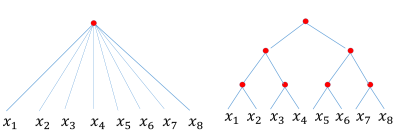
\includegraphics[scale=2.5]{../images/ComplexityNN.png}
\end{center}

\begin{itemize}
  \item $W_m^n$: class of $n$-variable functions with partial derivatives up to $m$-th order

  \item $W_m^{n,2}\subset W_m^n$: compositional subclass following binary tree structure

\end{itemize}

\textbf{Theorem.} Let $\sigma: \mathbb{R} \rightarrow \mathbb{R}$ be infinitely differentiable, and not a polynomial. For $f \in W_m^n$ the complexity of shallow networks that provide accuracy at least $\varepsilon$ is
$N=O\left(\varepsilon^{-n / m}\right)$ and is the best possible.\\ \\
\textbf{Theorem.} For $f \in W_m^{n, 2}$ consider a deep network with the same compositonal architecture and with an activation function $\sigma$ : $\mathbb{R} \rightarrow \mathbb{R}$ which is infinitely differentiable, and not a polynomial. The complexity of the network to provide approximation with accuracy at least $\varepsilon$ is

\begin{equation}
N=O\left((n-1) \varepsilon^{-2 / m}\right) .
\end{equation}

\textbf{Theorem.} Let $f$ be a L-Lipshitz continuous function of $n$ variables. Then, the complexity of a network which is a linear combination of ReLU providing an approximation with accuracy at least $\varepsilon$ is

$$
N_s=O\left(\left(\frac{\varepsilon}{L}\right)^{-n}\right)
$$

wheres that of a deep compositional architecture is

$$
N_d=O\left((n-1)\left(\frac{\varepsilon}{L}\right)^{-2}\right) .
$$

\section{Physics Informed Neural Networks (PINNs)}
Setting of the problem: consider $\Omega \subset \mathbb{R}^d$ and a PDE parametrized by $\lambda$ for the solution $u(x)$:
\[
    f\left(x; \dfrac{\partial u}{\partial x_1}, \dots, \dfrac{\partial u}{\partial x_d}; \dfrac{\partial^2 u}{\partial x_1 \partial x_1}, \dots, \dfrac{\partial^2 u}{\partial x_1 \partial x_d}, \dots, \dfrac{\partial^2 u}{\partial x_d \partial x_d}; \lambda\right) = 0, \hspace{0.5cm} x \in \Omega    
\]
And $\mathcal{B}(u,x) = 0$ on the boundary $\partial \Omega$. For time-dependent problems $t$ is considered as a special component of $x$ and $\Omega$ contains also the temporal domain. The IC are treated as a special type of Dirichlet BC on the spatio-temporal domain. 
The training set is:
\[
    \mathcal{T} = {x_1, x_2, \dots, x_{|\mathcal{T}|}} \text{ of size } |\mathcal{T}|    
\]
Residual points:
\[
    \mathcal{T}_f \subset \Omega \text{ and } |\mathcal{T}_b \subset \partial \Omega     
\]
Then, we have:
\[
    \mathcal{L}(\theta; \mathcal{T}) = w_f\mathcal{L}_f(\theta; \mathcal{T}_f) + w_b\mathcal{L}_b(\theta; \mathcal{T}_b)     
\]
Where
\[
    \mathcal{L}_f(\theta; \mathcal{T}_f) = \dfrac{1}{|\mathcal{T}_f|} \sum_{x \in \mathcal{T}_f} \left\|f\left(x; \dfrac{\partial u}{\partial x_1}, \dots, \dfrac{\partial u}{\partial x_d}; \dfrac{\partial^2 u}{\partial x_1 \partial x_1}, \dots, \dfrac{\partial^2 u}{\partial x_1 \partial x_d}, \dots, \dfrac{\partial^2 u}{\partial x_d \partial x_d}; \lambda\right)\right\|^2_2 
\]
\[
    \mathcal{L}_b(\theta; \mathcal{T}_b) = \dfrac{1}{|\mathcal{T}_b|} \sum_{x \in \mathcal{T}_b} \left\|\mathcal{B}(u,x)\right\|^2_2
\]
\begin{center}
    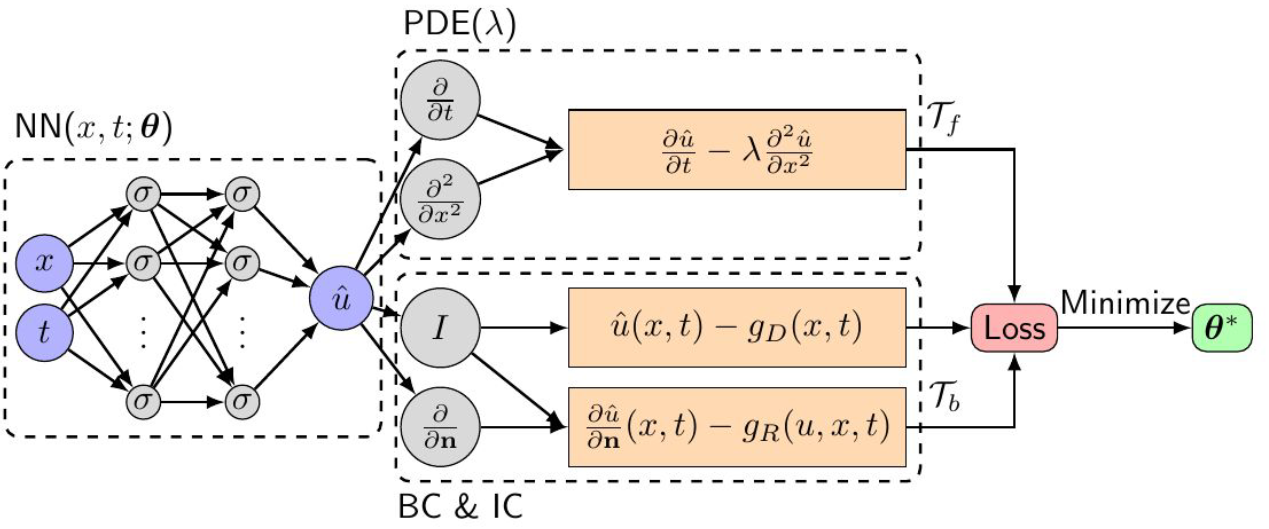
\includegraphics[scale=0.3]{../images/PINN_Architecture.png}
\end{center}
The actual PINN algorithm:
\begin{center}
    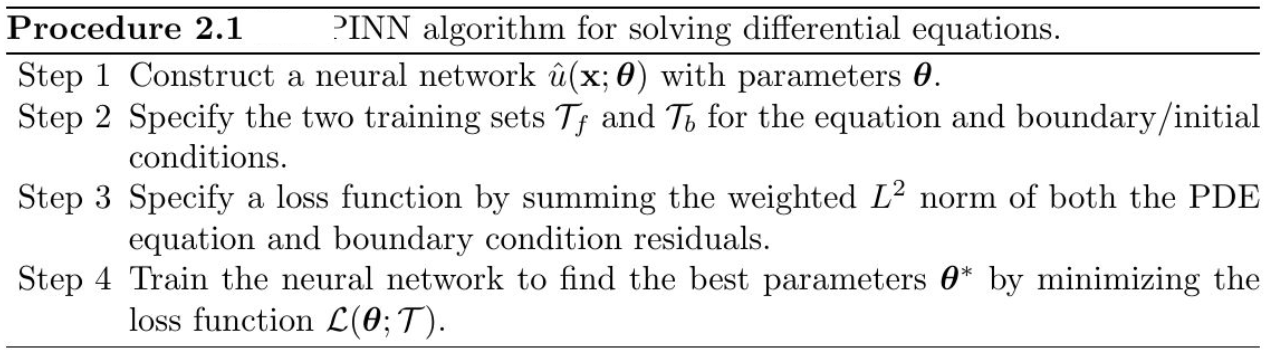
\includegraphics[scale=0.3]{../images/PINN_Algorithm.png}
\end{center}

\subsection*{Errors}
We define:
\begin{itemize}
    \item $\mathcal{F}$: family of all functions that can be represented by the chosen NN
    \item $u_{\mathcal{F}} = \arg \min_{f \in \mathcal{F}} \|f-u\|$: best function in $\mathcal{F}$ close to $u$
    \item $u_{\mathcal{T}} = \arg \min_{f \in \mathcal{F}} \mathcal{L}(\theta; \mathcal{T})$: solution given by the NN when the loss is at global minimum
    \item $\tilde{u}_{\mathcal{T}}$ = approximate solution returned by the optimizer
    \item $\varepsilon_{app}$: measures how closely $u_{\mathcal{F}}$ can approximate $u$
    \item $\varepsilon_{gen}$: is determined by the number and locations of residual points and by the capacity of the family $\mathcal{F}$
    \item $\varepsilon_{opt}$: is due to the loss function complexity and the optimization setup (learning rate, number of iterations, \dots)
\end{itemize}

\[
    \varepsilon := \|\tilde{u}_{\mathcal{T}} - u\| \leq \underbrace{\|\tilde{u}_{\mathcal{T}} - u_{\mathcal{T}}\|}_{\varepsilon_{opt}} + \underbrace{\|u_{\mathcal{T}} - u_{\mathcal{F}}\|}_{\varepsilon_{gen}} + \underbrace{\|u_{\mathcal{F}} - u\|}_{\varepsilon_{app}}    
\]
\begin{center}
    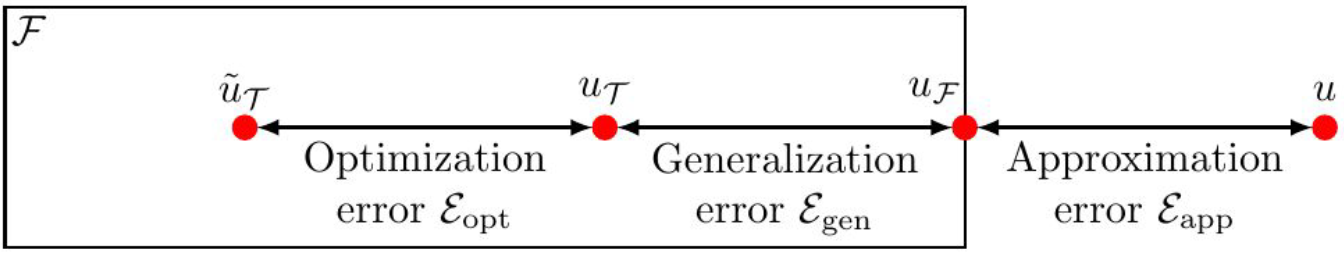
\includegraphics[scale=0.3]{../images/PINN_Error.png}
\end{center}
Comparison between PINN and FEM:
\begin{center}
    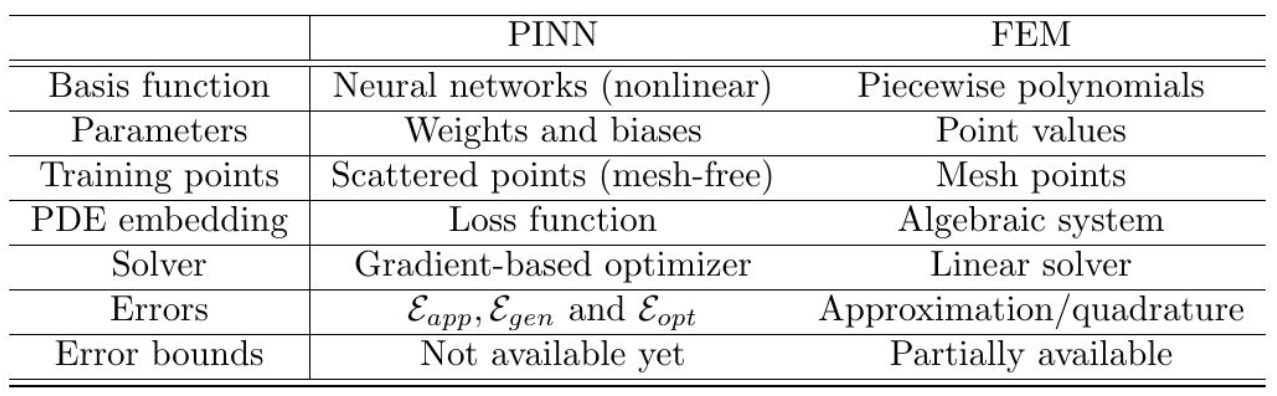
\includegraphics[scale=0.3]{../images/PINN_FEM_Comparison.png}
\end{center}

\subsection*{NS cylinder}
\[
    \begin{cases}
        \nabla \cdot u = 0 & x \in \Omega, t \in (0, T]\\
        \dfrac{\partial u}{\partial t} - \nu \nabla^2 u + (u \cdot \nabla)u + \nabla p = f & x \in \Omega, t \in (0, T]\\
    \end{cases}
\]
\begin{center}
    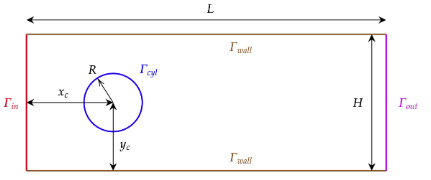
\includegraphics[scale=0.3]{../images/NS_Cylinder1.png}
\end{center}
\begin{center}
    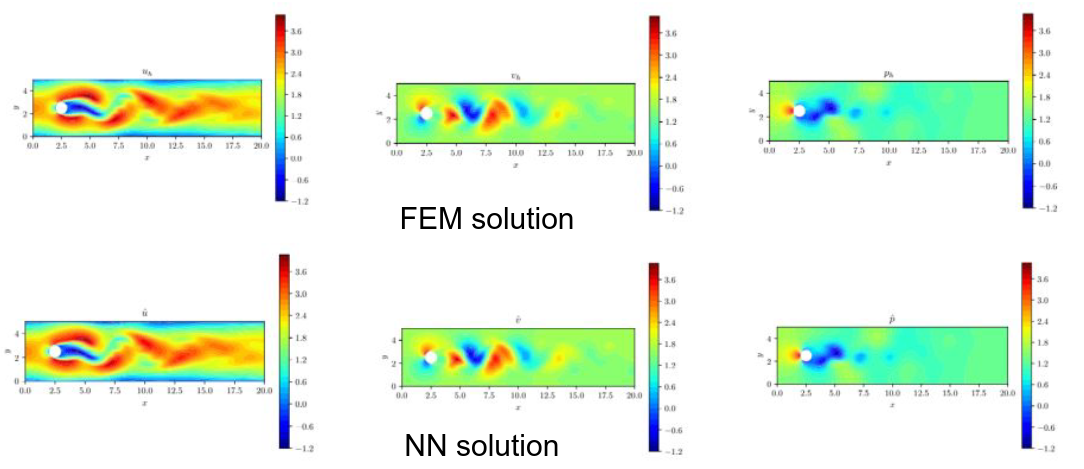
\includegraphics[scale=0.3]{../images/FEM_PINN_Solution.png}
\end{center}

\subsection*{PINNs for inverse problems}
Inverse problem: presence of unknown parameters $\lambda$ and some extra information on points $\mathcal{T}_i \subset \Omega$:
\[
    \mathcal{I}(u,x) = 0 \hspace{0.3cm}\text{for } x \in \mathcal{T}_i    
\]
\[
    \mathcal{L}(\theta, \lambda; \mathcal{T}) = w_f \mathcal{L}_f(\theta, \lambda; \mathcal{T}_f) + w_b \mathcal{L}_b(\theta, \lambda; \mathcal{T}_b) + w_i \mathcal{L}_i(\theta, \lambda; \mathcal{T}_i)    
\]
Where
\[
    \mathcal{L}(\theta, \lambda; \mathcal{T}_i) = \dfrac{1}{|\mathcal{T}_i|} \sum_{x \in \mathcal{T}_i} \left\|\mathcal{I}(\hat{u},x)\right\|^2_2
\]
\section{Appendix}
\subsection*{Functional Analysis}
A real vector space VV is a set with operations +:V×V→V+ : V \times V \to V and ⋅:R×V→V\cdot: \mathbb{R}\times V \to V such that:

\begin{itemize}
    \item u+v=v+uu + v = v + u (commutativity of vector addition)
    \item (u+v)+w=u+(v+w)(u + v) + w = u + (v + w) (associativity of vector addition)
    \item There exists an element 0∈V0 \in V such that v+0=vv + 0 = v for all v∈Vv \in V (existence of zero vector)
    \item For every v∈Vv \in V, there exists an element −v∈V-v \in V such that v+(−v)=0v + (-v) = 0 (existence of additive inverses)
    \item λ⋅(u+v)=λ⋅u+λ⋅v\lambda \cdot (u + v) = \lambda \cdot u + \lambda \cdot v (distributivity of scalar multiplication over vector addition)
    \item (λ+μ)⋅v=λ⋅v+μ⋅v(\lambda + \mu) \cdot v = \lambda \cdot v + \mu \cdot v (distributivity of scalar multiplication over real addition)
    \item (λμ)⋅v=λ⋅(μ⋅v)(\lambda \mu) \cdot v = \lambda \cdot (\mu \cdot v) (associativity of scalar multiplication)
    \item $1 \cdot v = v$ (scalar multiplication identity)
\end{itemize}


Examples of real vector spaces are: $\mathbb{R}^n$, $P_K(I)$: set of polynomials of order $\leq K$ on the interval $I$, $C^k(I)$: set of functions with $k$ continuous derivatives on the interval $I$.\\

A basis for the vector space $V$ is the minimal set of vectors (basis function) that span $V$. The basis functions must be \textbf{linearly independent} and the number of basis functions is the \textbf{dimension} of the vector space. Any vector $v \in V$ can be written as a linear combination of the basis functions:
\[
    v = c_1 \phi_1 + c_2 \phi_2 + \dots + c_n \phi_n    
\]

\textbf{Example}: the dimension of $P_K)I=$ is $K+1$ and the basis functions are $\{1,x,x^2,\dots,x^K\}$.\\

Let $V$ be a vector space over $\mathbb{R}$. An inner product $(,)$ is a function $V \times V \to \mathbb{R}$ with the following properties:
\begin{enumerate}
    \item $\forall u \in V, (u,u) \geq 0 $ and $(u,u) = 0 \iff u = 0$
    \item $\forall u,v \in V, (u,v) = (v,u)$
    \item $\forall u,v,w \in V$ and $\forall \alpha,\beta \in \mathbb{R}, (\alpha u + \beta v, w) = \alpha(u,w) + \beta(v,w)$
\end{enumerate}
$V$ together with $(,)$ is called an \textbf{inner product space}.\\

\textbf{Example}: Given two vectors in $\mathbb{R}^2: v = v_1e_1 + v_2e_2$ and $w = w_1e_1 + w_2e_2$, the Euclidean inner product in $\mathbb{R}^2$ is:
\[
    (v,w) = v_1w_1 + v_2w_2     
\]
The extension to $\mathbb{R}^n$ is obvious.\\

\textbf{Example}: An inner product in the vector space of continuous functions in [0,1] ($C([0,1])$) is:
\[
    (f,g) = \int_0^1 f(x)g(x)dx    
\]
where $f,g \in C([0,1])$.\\

\textbf{Example}: An inner product in the vector space of functions with one continuous derivative in [0,1] ($C^1([0,1])$) is:
\[
    (f,g) = \int_0^1 f(x)g(x) + f'(x)g'(x)dx    
\]
where $f,g \in C^1([0,1])$.\\

\textbf{Remark}: an inner product induces a norm $\|f\| = \sqrt{(f,f)}$.\\

A norm on a vector space $V$ is a mapping $\|\cdot\|: V \to \mathbb{R}$ that satisfies:
\begin{enumerate}
    \item $\|u\| \geq 0$ and $\|u\| = 0 \iff u = 0$
    \item $\|\alpha u\| = |\alpha|\|u\|$
    \item $\|u+v\| \leq \|u\| + \|v\|$
\end{enumerate}
This is valid $\forall u,v \in V $ and $\forall \alpha \in \mathbb{R}$.\\
A normed vector space is a vector space equipped with a norm. 
\begin{itemize}
    \item Norms in $\mathbb{R}^n$:
    \[
        \|v\|_p = \left(\sum_{i=1}^{n} |v_i|^p\right)^{1/p}   \hspace{1cm} \|v\|_1 = \sum_{i=1}^{n} |v_i| \hspace{1cm} \|v\|_\infty = \max_{i=1,\dots,n} |v_i|
    \]
    \item Norms in $C^0(I)$ and $P_K(I)$:
    \[
        \|v\|_{L^p(I)} = \left(\int_I |v|^p dx\right)^{1/p}   \hspace{1cm} \|v\|_{L^{\infty}(I)} = \sup_{x \in I} |v(x)| 
    \]
\end{itemize}

A \textbf{bilinear form} on a vector space $V$ is mapping a $a(\cdot,\cdot) = V \times V \to \mathbb{R}$ such that:
\begin{itemize}
    \item $a(u+v,w) = a(u,w) + a(v,w)$
    \item $a(u,v+w) = a(u,v) + a(u,w)$
    \item $a(\lambda u, v) = \lambda a(u,v)$
    \item $a(u,\lambda v) = \lambda a(u,v)$
\end{itemize}
This is valid $\forall u,v,w \in V$ and $\forall \lambda \in \mathbb{R}$. The bilinear form is symmetric if $a(u,v) = a(v,u)$ $\forall u,v \in V$ and continuous, or bounded, if there is a constant $C$ such that $|a(u,v)| \leq C\|u\|\|v\|$ $\forall u,v \in V$.\\

A symmetric bilinear form $a(\cdot,\cdot)$ is called an inner product if $a(u,u) \geq 0$ with equality if and only if $u=0$ $\forall u \in V$. Inner products are often also denoted $(\cdot,\cdot)$. An inner product defines a so-called induced norm by:
\[
    \|u\|^2 = (u,u)    
\]
on the vector space $V$. In particular, $a(\cdot,\cdot)$ defines the induced energy norm $\||u\||^2 = a(u,u)$. A vector space equipped with an inner product is called an inner product space. In such spaces the Cauchy-Schwarz inequality:
\[
    |(u,v)| \leq \|u\|\|v\|    
\]
holds for all $u,v \in V$.\\

A \textbf{Cauchy sequence} in a normed vector space $V$ is a sequence $\{v_i\}^{\infty}_{i=1}$ of elements $v_i \in V$ such that
 \[
    \forall \epsilon > 0 \hspace{0.2cm} \exists N \in \mathbb{N} \hspace{0.2cm}\text{such that}\hspace{0.2cm} \|v_i - v_j\| < \epsilon \hspace{0.2cm}\forall i,j \geq N
\] 
A normed vector space is called complete if every Cauchy sequence in $V$ converges to an element in $V$.\\

\textbf{Remark}: a convergent sequence is a Cauchy sequence. The converse is not true. Indeed, there are Cauchy sequences that do not converge in their space. For example, the sequence of rational numbers $(u_n)_{n \in \mathbb{N}} \in \mathbb{Q}$ given by:
\[
    u_n = \dfrac{1}{0!} + \dfrac{1}{1!} + \dots + \dfrac{1}{n!}    
\]
is Cauchy in $\mathbb{Q}$ but converges to the constant $e$, which belongs to $\mathbb{R}$ but not to $\mathbb{Q}$.\\

\textbf{Definition:} a vector space is said to be complete if every Cauchy sequence is also convergent.\\

\textbf{Definition:} a Banach space is a complete normed vector space.\\

\textbf{Definition:} a Hilbert space is a complete inner product space.\\

\begin{center}
    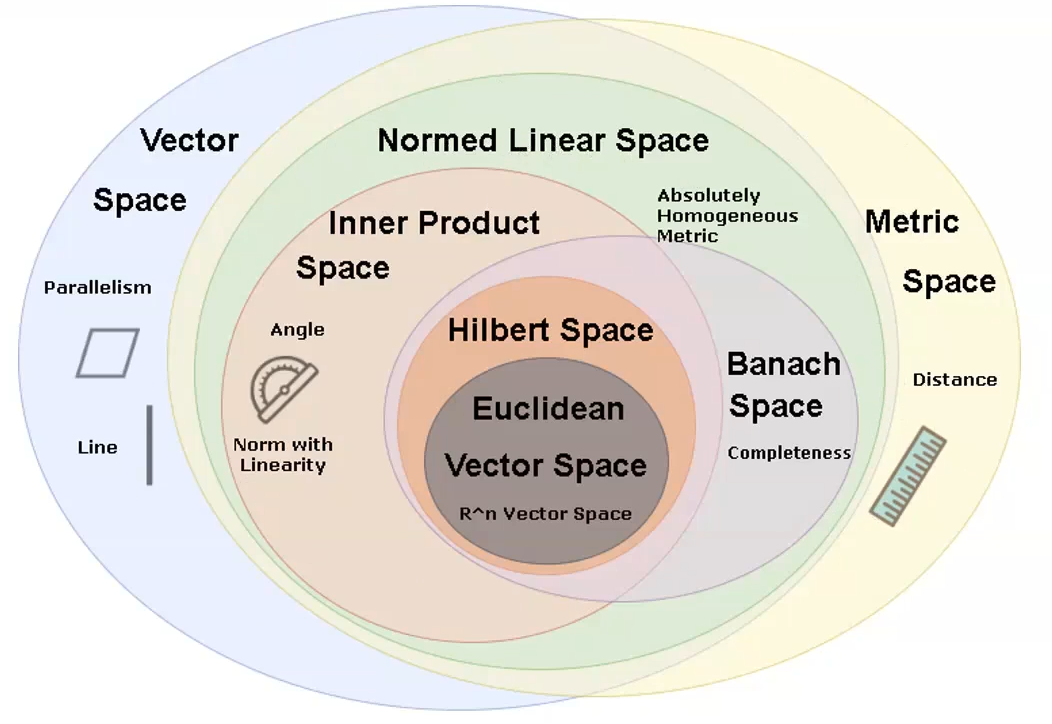
\includegraphics[scale = 0.2]{../images/SetsSpace.png}
\end{center}

\subsection*{Riemann integral}
For a function to be Riemann integrable, the infimum of the upper Riemann sum and the supremum of the lower Riemann sum should be the same.
\[
    m_k = \inf\{f(t):x_{k-1} \leq t\leq x_k\} \hspace{1cm} M_k = \sup\{f(t):x_{k-1} \leq t\leq x_k\}    
\]
\[
    L(f,P) = \sum_{k=1}^N m_k(x_k - x_{k-1}) \hspace{1cm} U(f,P) = \sum_{k=1}^N M_k(x_k - x_{k-1})    
\]
Is Riemann integral ok? Consider:
\[
    \mathbbm{1}_{\mathbb{Q}} = \begin{cases}
        1 & x \in \mathbb{Q}\\
        0 & x \notin \mathbb{Q}
    \end{cases}    
\]
In this case: $L(f,P) = 0 \neq 1 = U(f,P)$. So the function is not Riemann integrable. 

\subsection*{Lebesque integral}
Is defined as follows: 
\[
    \int_{\mathbb{R}}\phi dm := \sum_{i=1}^{n} a_i m(S_i)    
\]
Here, instead of having a partition of the interval, we have a partition of the set. The function $\phi$ is the characteristic function of the set $S_i$ and $a_i$ is the value of the function in the set $S_i$. \textbf{We are still computing a "rectangular" area but this time the base is not fixed to a certain "dx" (or $\Delta x$) but it is the measure of the set $S_i$ which can be large. The total area is not computed by stacking side to side small and tall rectangulars but by stacking on over the other larger and shorter (of height $a$)rectangulars}.\\
\begin{multicols}{2}
    \begin{center}
        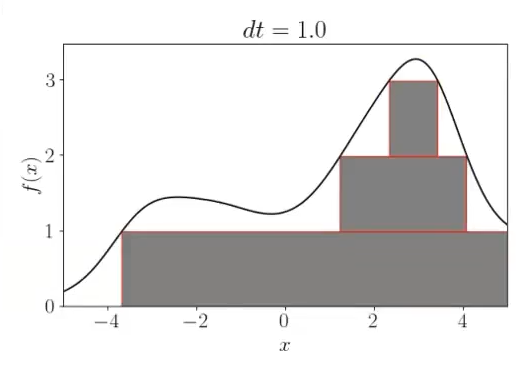
\includegraphics[scale = 0.4]{../images/LebesgueIntegral.png}
    \end{center}
    \begin{center}
        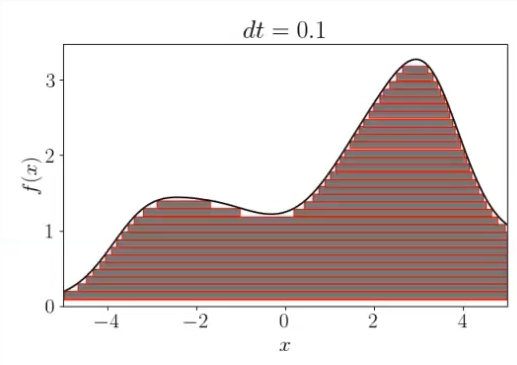
\includegraphics[scale = 0.4]{../images/LebesgueThinner.png}
    \end{center}
\end{multicols}
Of course, as it was done in Riemann integral, you will reach a better approximation of the area by considering thinner and thinner layers of rectangulars.
\textbf{We need to define the concept of "measure"!}\\

\textbf{Theorem:} every countable set has measure 0.\\

The integral with Lebesque is easy: $1\times S_1 + 0\times S_2$ where $S_1$ is the set of all irrational numbers in [0,1] and $S_2$ is the set of rational numbers. $S_2$ is countable so $\mu(S_2) = 0$ moreover since $S_1$ and $S_2$ are disjoint we have $\mu([0,1]) = 1 \implies \mu(S_1) = \mu([0,1] - \mu(S_2)) = 1 - 0 = 1$. So the integral is 1!

\textbf{Remark:} if a function is Riemann integrable then it is also Lebesque integrable and the two integrals coincide. The converse is not true.\\

With the Lebesque integral we can define the $L^p$ spaces:  
\[
    L^p(|\Omega) = \{v: \Omega \to \mathbb{R}: \|v\|_{L^p(\Omega)} < \infty\}    
\]
So the space $L^p$ is the set of functions which have norm which is bounded. The norm is defined as:
\[
    \|v\|_{L^p(\Omega)} = \left(\int_{\Omega} |v|^p dm\right)^{1/p}
\]
With $1 \leq p \leq \infty$. In particular, if $p = \infty$ we have:
\[
    \|v\|_{L^\infty(\Omega)} = \sup_{x \in \Omega} |v(x)|    
\]

\textbf{Remark:} the $L^p(\Omega)$ spaces are Banach spaces for $1 \leq p \leq \infty$.\\

\textbf{Remark:} The space $L^2(\Omega)$ is a Hilbert space, as its norm $\|v\|_{L^2(\Omega)}$ is induced by the inner product $(v,w)_{L^2(\Omega)} = \int_{\Omega} vw \, dx$. However, for $p \neq 2$, the space $L^p(\Omega)$ is only a Banach space, as its norm $\|v\|_{L^p(\Omega)}$ is not induced by an inner product.
\begin{center}
    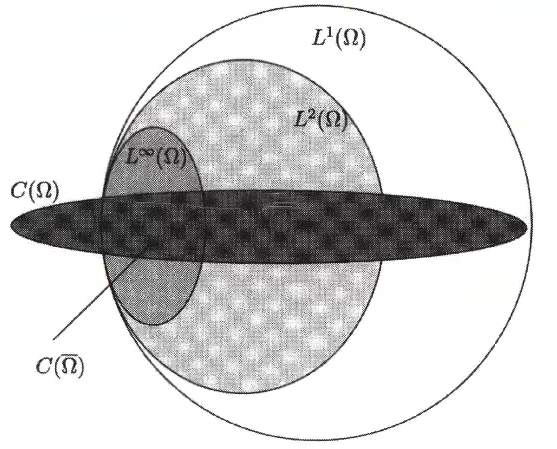
\includegraphics[scale = 0.35]{../images/LpSpaces.png}
\end{center}
In the picture there is also $C(\Omega)$ which corresponds to the set of continuous functions in $\Omega$. $\bar{\Omega}$ is the closure of $\Omega$.\\

Suppose have this differential problem:
\[
    \begin{cases}
        -u''(x) = f(x) & x \in (0,1)\\  
        u(0) = u(1) = 0
    \end{cases}    
\]
This, for example, is a model for an elastic string and $f$ is some sort of external force applied to it. We have 3 different external forces as shown in the figure here:
\begin{center}
    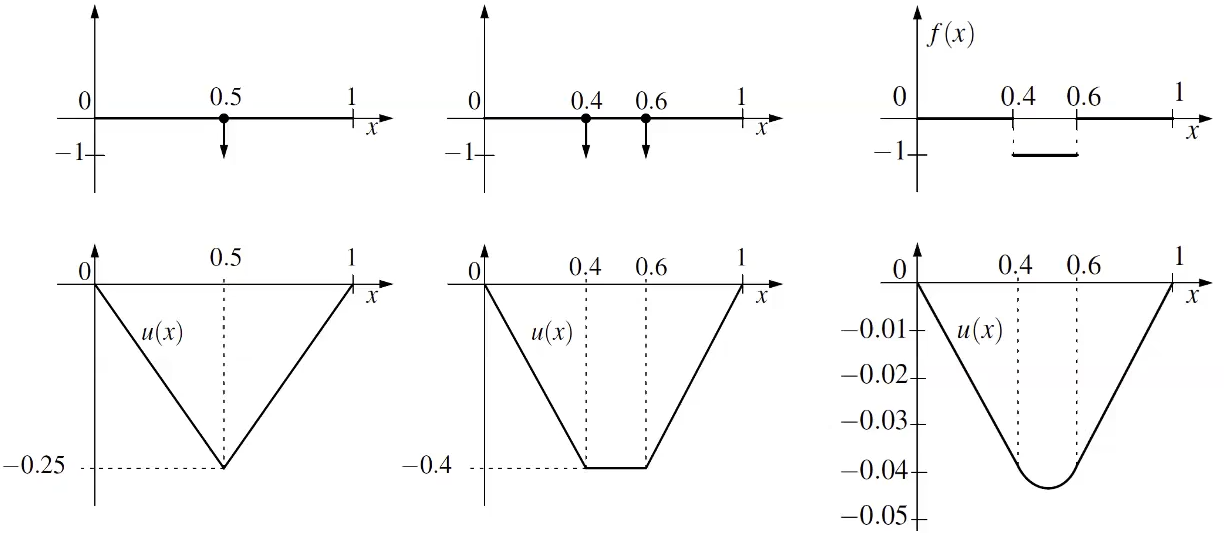
\includegraphics[scale = 0.35]{../images/ExternalForces.png}    
\end{center}
In the first case the force is all concentrated in the point 0.5, in the second case the force is distributed in the two points 0.4 and 0.6 while in the third case the force is distributed in the whole interval.In the bottom of the picture there are the solutions of the three problems. But, as you can see, the functions $u(x)$ are not differentiable.

There is a contraddiction: the physical problem admits a solution which is not coherent with the regularity required by the differential problem. We have to rethink the definition of derivative, we have to introduce the concept of \textbf{weak derivative}.\\

\subsection*{Weak derivatives}
Functions in Hilbert spaces are not regular enough for the standard definition of derivative to make sense. 
\begin{itemize}
    \item $C^k(\Omega)$: space of all $k < \infty$ times continuously differentiable functions in $\Omega$.
    \item $\mathcal{D}(\Omega) = \{\varphi \in C^\infty(\Omega) \text{with compact support in }\Omega\}$
    \item $\alpha = (\alpha_1, \dots, \alpha_d)$ is a multi-index, i.e. d-tuple of non negative integers
    \item $|\alpha| = \alpha_1 + \dots + \alpha_d = \sum_{i=1}^{d} \alpha_i$: order of the multi-index
    \item $D^\alpha \phi = \prod\limits_{i=1}^{d}\left(\dfrac{\partial}{\partial x_i}\right)^{\alpha_i} \varphi$, \hspace{0.1cm} $\varphi \in \mathcal{D}(\Omega)$
\end{itemize}
So, if we have to compute $\frac{\partial u}{\partial x_i}$ we can:
\[
    \int_{\Omega} \dfrac{\partial u}{\partial x_i} \varphi dx =  - \int_{\Omega} u \dfrac{\partial \varphi}{\partial x_i} dx \hspace{1cm} \forall \varphi \in \mathcal{D}(\Omega), \text{ for any } u \in C^1(\Omega)    
\]
We multiply by $\varphi$ which is an infinitely regular function then by integration by parts and by noticing that $\varphi$ has compact support so it is 0 outside a certain interval we can rewrite the integral and the derivative of $u$ has been transfered over $\varphi$ which is regular enough to take all the derivatives that you want. If you iterate this you can define:
\[
    \int_{\Omega} (D^\alpha u)\varphi dx = (-1)^{|\alpha|}\int_{\Omega} u(D^\alpha \varphi) dx \hspace{1cm} \forall \varphi \in \mathcal{D}(\Omega), \text{ for any } u \in C^{|\alpha|}(\Omega)    
\]
In practice, we usually define the following space which is the set of functions $v$ which are in $L^1(K)$ where $K$ is a subset of $\Omega$ on which the function is different than 0 inside and equal to 0 outside: 
\[
    L_{loc}^{1}(\Omega) = \{v:v\in L^1(K)\hspace{0.1cm} \forall K \text{ compactly supported in }\Omega \}    
\]
Let $u \in L^1_{loc}(\Omega)$ (function $u$ that belongs to that set), if there is a function $g \in L^1_{loc}(\Omega)$ such that:
\[
    \int_{\Omega} g\varphi dx = (-1)^{|\alpha|} \int_{\Omega} u(D^\alpha \varphi) dx \hspace{1cm} \forall \varphi \in \mathcal{D}(\Omega)    
\]
then we say that $g$ is the weak derivative $D^\alpha u$ of $u$.
So, essentially, apart from the formalism, the idea is that the weak derivative amounts to take the derivative you want to compute, multiply by a function which is regular enough, apply many times ($\alpha$ in general) the integration by parts and, due to the fact that the function $\varphi$ is compactly supported, then you can end up with the final relation.\\

\textbf{Remark:} weak and classical derivatives share many properties, such as linearity, the chain rule and the differentiation of products, for instance. \\



\end{document}